\documentclass[a4paper]{report}
\title{{\LARGE Detailed formulation of SCALE-RM}}
\author{Seiya Nishizawa, Hirofumi Tomita, and Team SCALE}
\date{\today}

\usepackage[dvipdfmx]{graphicx}
\usepackage[dvipdfmx]{hyperref}
\usepackage{amsmath}
\usepackage{siunitx}
\usepackage[round]{natbib}
\usepackage{bm}
\usepackage{url}
\usepackage{pxjahyper}
\hypersetup{% options for hyperref
 bookmarksopen=true,
 bookmarksnumbered=true,
 colorlinks=true,
% linkcolor=red,
 linkcolor=cyan,
 citecolor=cyan,
 urlcolor=cyan,
}


\begin{document}
\maketitle
\tableofcontents

\chapter{Introduction}
%{\bf \Large
%\begin{tabular}{ccc}
%\hline
%  Corresponding author & : & ???\\
%\hline
%\end{tabular}
%}


\section{What is SCALE}
SCALE (Scalable Computing for Advanced Library and Environment)is a basic library of weather and climate models of the earth and planets intended for widespread use.
The SCALE library was co-designed by computational science and computer science researchers.



\chapter{Governing equations}
\chapter{Governing equations}
{\bf \Large 
\begin{tabular}{ccc}
\hline
  Correnspoinding author & : & Hirofumi Tomita\\
\hline
\end{tabular}
}

\section{Continuity equations}

The continuity equations for each material can be described as the flux form:
\begin{eqnarray}
&&  \frac{\partial \rho q_d}{\partial t}
+ \nabla \cdot\left(\rho q_d{\bf u}\right)  = {\rm DIFF}\left[q_d\right]
\label{eq:rho_d}\\
&&  \frac{\partial \rho q_v}{\partial t}
+ \nabla \cdot\left(\rho q_v {\bf u}\right)  = S_v + {\rm DIFF}\left[q_v\right]
\label{eq:rho_v}\\
&&  \frac{\partial \rho q_l}{\partial t}
+ \nabla \cdot\left(\rho q_l {\bf u}\right)
+ \frac{\partial \rho q_l w_l}{\partial z}=S_l + {\rm DIFF}\left[q_l\right]
\label{eq:rho_l}\\
&&  \frac{\partial \rho q_s}{\partial t}
+ \nabla \cdot\left(\rho q_s {\bf u}\right)
+ \frac{\partial \rho q_s w_s}{\partial z}=S_s + {\rm DIFF}\left[q_s\right]
\label{eq:rho_s}
\end{eqnarray}
The summation of the mass concentrations should be unit:
\begin{eqnarray}
&& q_d + q_v + q_l + q_s = 1. \label{eq:total_massconcentration}
\end{eqnarray}
The source terms of water substances should satisfy the following relation:
\begin{eqnarray}
  S_v + S_l + S_s = 0.
\end{eqnarray}
The summation of Eqs.(\ref{eq:rho_d})-(\ref{eq:rho_s}) gives the
continuity equation of total density:
\begin{eqnarray}
&&  \frac{\partial \rho}{\partial t}
+ \nabla\cdot\left(\rho{\bf u}\right) 
+ \frac{\partial \rho q_l w_l}{\partial z}
+ \frac{\partial \rho q_s w_s}{\partial z}
=0, \label{eq:rhotot}
\end{eqnarray}
For this derivation,
we assume that 
the operator ${ \rm DIFF}\left[\right]$ is distributive.
Using Eq.(\ref{eq:total_massconcentration}),
\begin{eqnarray}
&&  { \rm DIFF}\left[q_d\right]
+{ \rm DIFF}\left[q_v\right]
+{ \rm DIFF}\left[q_l\right]
+{ \rm DIFF}\left[q_s\right]\nonumber\\
&=&{ \rm DIFF}\left[q_d+q_v+q_l+q_s\right]
={ \rm DIFF}\left[1\right] = 0
\end{eqnarray}

\section{Momentum equations}

The momentum equations for the gas, liquid, and solid material 
are described as
\begin{eqnarray}
&&  \frac{\partial \rho \left(q_d+q_v\right) {\bf u}}{\partial t}
+ \nabla \cdot \left[\rho \left(q_d+q_v\right){\bf u} \otimes {\bf u}\right]\\
&=& 
-\nabla p - \left[\rho \left(q_d+q_v\right)g + (f_l+f_s)\right] {\bf e_z}\nonumber\\
&&+{\bf u} S_v +{\rm DIFF}\left[(q_d+q_v){\bf u}\right]
\label{eq:momgas}\\
&&  \frac{\partial \rho q_l {\bf u}}{\partial t}
+ \nabla \cdot \left(\rho q_l{\bf u} \otimes {\bf u}\right)  
+ \frac{\partial \rho q_l {\bf u} w_l}{\partial z}
= 
 - \left(\rho q_l g - f_l\right) {\bf e_z}\nonumber\\
&&+{\bf u} S_l+{\rm DIFF}\left[q_l{\bf u}\right]
\label{eq:momliquid}\\
&&  \frac{\partial \rho q_s {\bf u}}{\partial t}
+ \nabla \cdot \left(\rho q_s{\bf u} \otimes {\bf u}\right)  
+ \frac{\partial \rho q_s {\bf u }w_s}{\partial z}
= 
 - \left(\rho q_s g - f_s\right) {\bf e_z}\nonumber\\
&&+{\bf u} S_s+{\rm DIFF}\left[q_s{\bf u}\right]
\label{eq:momsolid}
\end{eqnarray}
The pressure is derived from the equation of state as
\begin{eqnarray}
p=\rho \left(q_d R_d + q_v R_v\right) T.\label{eq:state}
\end{eqnarray}
The summation of Eqs.(\ref{eq:momgas})-(\ref{eq:momsolid})
gives the total momentum equation as
\begin{eqnarray}
&&  \frac{\partial \rho {\bf u}}{\partial t}
+ \nabla \cdot \left(\rho{\bf u} \otimes {\bf u}\right)  
+ \left(\frac{\partial \rho q_l w_l}{\partial z}
+ \frac{\partial \rho q_s w_s}{\partial z}\right) {\bf e_z}\nonumber\\
&=&
-\nabla p - \rho g {\bf e_z} 
+{\rm DIFF}\left[{\bf u}\right]
\label{eq:momtot}
\end{eqnarray}
Note that the drag forces by water loading does not appear
in Eq.(\ref{eq:momtot}), 
because those term are cancelled out through the summation. 

\section{Thermodynamics equations}

The equations of the internal energies are described as
\begin{eqnarray}
&&  \frac{\partial \rho (q_d e_d + q_v e_v) }{\partial t} + 
  \nabla \cdot \left[ \rho (q_d e_d + q_v e_v ){\bf u} \right] \nonumber\\
&=& - p \nabla \cdot {\bf u} + Q_{d}+ Q_{v} + {\rm DIFF}\left[(q_d+q_v)T^{*} \right]
\label{eq:thermogas}\\
&&  \frac{\partial \rho q_l e_l}{\partial t} + 
  \nabla \cdot \left( \rho q_l e_l {\bf u} \right) 
+ \frac{\partial \rho q_l e_l w_l}{\partial z}
= Q_l + {\rm DIFF}\left[q_l T^{*} \right]
\label{eq:thermoliquid}\\
&&  \frac{\partial \rho q_l e_s}{\partial t} + 
  \nabla \cdot \left( \rho q_s e_s {\bf u} \right) 
+ \frac{\partial \rho q_s e_s w_s}{\partial z}
= Q_s + {\rm DIFF}\left[q_s T^{*} \right]
\label{eq:thermosolid}
\end{eqnarray}
where $T^*$ is some kind of potential temperature, discussed later.
The internal energies are defined as
\begin{eqnarray}
&& e_d = c_{vd} T\\
&& e_v = c_{vv} T\\
&& e_l = c_{l} T\\
&& e_s = c_{s} T,
\end{eqnarray}
The summation of Eqs.(\ref{eq:thermogas})-(\ref{eq:thermosolid})
gives the following internal energy equations:
\begin{eqnarray}
&&  \frac{\partial \rho e  }{\partial t}
+  \nabla \cdot \left( \rho e {\bf u} \right)
+ \frac{\partial \rho q_l e_l w_l}{\partial z}
 + \frac{\partial \rho q_s e_s w_s}{\partial z}
 + p \nabla \cdot {\bf u}\nonumber\\
&=&  Q + {\rm DIFF}\left[T^{*} \right]
\label{eq:etot}
\end{eqnarray}
where
\begin{eqnarray}
&&  e = q_d e_d + q_v e_v + q_l e_l + q_s e_s,
\end{eqnarray}
and the total diabatic heating is described as
\begin{eqnarray}
&&  Q = Q_d + Q_v + Q_l + Q_s.
\end{eqnarray}

\section{Conseptual seperation for solving the set of equations}

Eqs.(\ref{eq:rho_v})-(\ref{eq:rho_s}),(\ref{eq:rhotot}),(\ref{eq:momtot}),
and (\ref{eq:state}) with Eq.(\ref{eq:etot}) are the complete set of equations.
For solving them easily, we seperate the set of equations conceptually as
\begin{eqnarray}
&&  \frac{\partial \phi}{\partial t} = 
\left(\frac{\partial \phi}{\partial t}\right)_{dynamics}
+\left(\frac{\partial \phi}{\partial t}\right)_{physics}\\
&&\phi^{*} = \phi^{n} + 
\Delta t \left(\frac{\partial \phi}{\partial t}\right)_{dynamics}\\
&&\phi^{n+1} = \phi^{*} + 
\Delta t \left(\frac{\partial \phi}{\partial t}\right)_{physics}
\end{eqnarray}
The falling proccess of liquid and solid waters,
the source and sink process of water vapor, and
the diabatic heating process for energy equations are treated
as physical process, the others are treated as dynamical proccess.

According to this scheme,
the dynamical process can be written as
\begin{eqnarray}
&&  \frac{\partial \rho q_v}{\partial t}
+ \nabla \cdot\left(\rho q_v {\bf u}\right)  = 0
\label{eq:rho_v_d}\\
&&  \frac{\partial \rho q_l}{\partial t}
+ \nabla \cdot\left(\rho q_l {\bf u}\right) = 0
\label{eq:rho_l_d}\\
&&  \frac{\partial \rho q_s}{\partial t}
+ \nabla \cdot\left(\rho q_s {\bf u}\right)
= 0
\label{eq:rho_s_d}\\
&&  \frac{\partial \rho}{\partial t}
+ \nabla\cdot\left(\rho{\bf u}\right) 
=0 \label{eq:rhotot_d}\\
&&  \frac{\partial \rho {\bf u}}{\partial t}
+ \nabla \cdot \left(\rho{\bf u} \otimes {\bf u}\right)  
= 
-\nabla p - \rho g {\bf e_z} \label{eq:momtot_d}\\
&&  \frac{\partial \rho e  }{\partial t}
+  \nabla \cdot \left( \rho e {\bf u} \right)
 + p \nabla \cdot {\bf u}
=  0 \label{eq:etot_d}
\end{eqnarray}

On the other hand, 
the physical processes are as follows:
\begin{eqnarray}
&&  \frac{\partial \rho q_v}{\partial t}  = S_v
+{\rm DIFF}\left[q_v \right]
\label{eq:rho_v_p}\\
&&  \frac{\partial \rho q_l}{\partial t}
+ \frac{\partial \rho q_l w_l}{\partial z}=S_l
+{\rm DIFF}\left[q_l \right]
\label{eq:rho_l_p}\\
&&  \frac{\partial \rho q_s}{\partial t}
+ \frac{\partial \rho q_s w_s}{\partial z}=S_s
+{\rm DIFF}\left[q_s \right]
\label{eq:rho_s_p}\\
&&  \frac{\partial \rho}{\partial t}
+ \frac{\partial \rho q_l w_l}{\partial z}
+ \frac{\partial \rho q_s w_s}{\partial z}
=0 \label{eq:rhotot_p}\\
&&  \frac{\partial \rho {\bf u}}{\partial t}
+ \frac{\partial \rho q_l {\bf u} w_l}{\partial z}
+ \frac{\partial \rho q_s {\bf u} w_s}{\partial z}
= {\rm DIFF}\left[{\bf u} \right] 
 \label{eq:momtot_p}\\
&&  \frac{\partial \rho e  }{\partial t}
+ \frac{\partial \rho q_l e_l w_l}{\partial z}
 + \frac{\partial \rho q_s e_s w_s}{\partial z}
=  Q + {\rm DIFF}\left[T^{*} \right] \label{eq:etot_p}
\end{eqnarray}

\section{Conservation of thermodynamics in the dynamical process}

Equation (\ref{eq:etot_d}) is not a complete flux form,
because the internal energy itself is not conserved
both in the Euler sense and in the Lagrangian sense.
In this section, we consider the conservative 
quantity for thermodynamics equation.

In the dry atmosphere, the potential temperature for dry air,
which is defined as
\begin{eqnarray}
\theta_d &=& T \left(\frac{p_{00}}{p}\right)^{R_d/c_{pd}},
\end{eqnarray}
is used as a conserved quantity it is conserved along the Lagrange trajectory
$c_{pd}$ $R_d$ are the specific heats at constant pressure and
However, it is no longer satisfied when the water substances are included.

Sinece Eq.(\ref{eq:rhotot_d}) is equivallent to
\begin{eqnarray}
  \frac{d \rho}{dt}+\rho \nabla \cdot {\bf u} = 0,
\end{eqnarray}
Equation (\ref{eq:etot_d}) is
\begin{eqnarray}
  \rho \frac{de}{dt} - \frac{p}{\rho}\frac{d \rho}{dt} =0. \label{eq:etot_d2}
\end{eqnarray}
Dividing by $\rho$, this equation can be written as
\begin{eqnarray}
  \frac{de}{dt} + p \frac{d}{dt}\left(\frac{1}{\rho}\right) = 0.
\label{eq:thermodyn}
\end{eqnarray}
Substiting Eq.(\ref{eq:state}) into Eq.(\ref{eq:thermodyn}),
\begin{eqnarray}
&& \frac{d  q_d c_{vd}   T}{dt} + p \frac{d}{dt} \left[\frac{q_d R_d T}{p}\right]
+\frac{d  q_v c_{vv}   T}{dt} + p \frac{d}{dt} \left[\frac{q_v R_v T}{p}\right]
\nonumber\\
&&+\frac{d  q_l c_{l}   T}{dt}+\frac{d  q_s c_{s}   T}{dt} =0 
\label{eq:thermodyn_dash}
\end{eqnarray}

Since Eqs.(\ref{eq:rho_v_d})-(\ref{eq:rhotot_d}) give
\begin{eqnarray}
  \frac{d q_d}{dt} = \frac{d q_v}{dt} = \frac{d q_l}{dt} = \frac{d q_s}{dt} = 0,
\end{eqnarray}
Equation (\ref{eq:thermodyn_dash}) gives the following form:
\begin{eqnarray}
&& q_d  \left[\frac{d  c_{vd}   T}{dt} +  p \frac{d}{dt} \left[\frac{ R_d T}{p}\right]\right]
+q_v \left[\frac{d  c_{vv}   T}{dt} + p \frac{d}{dt} \left[\frac{ R_v T}{p}\right]\right]\nonumber\\
&&+ q_l  \frac{d  c_{l}   T}{dt} + q_s  \frac{d  c_{s}   T}{dt} =0
\end{eqnarray}
Dividing this equation by $T$,
\begin{eqnarray}
%1
&&q_d  \left[c_{pd} \frac{1}{T}\frac{d T}{dt} 
+  R_d p \frac{d}{dt} \left(\frac{1}{p}\right)\right]
+q_v  \left[c_{pv} \frac{1}{T}\frac{d T}{dt} 
+  R_v p \frac{d}{dt} \left(\frac{1}{p}\right)\right]\nonumber\\
&&+ q_l c_{l} \frac{1}{T}  \frac{d   T}{dt}
  + q_s c_{s} \frac{1}{T}  \frac{d   T}{dt} =0\\
%2
&&q_d c_{pd} \left[ \frac{d \ln T}{dt} 
+  \frac{R_d}{c_{pd}} \frac{d}{dt} \left[\ln \left(\frac{1}{p}\right)\right]\right]
+q_v c_{pv}  \left[\frac{d \ln T}{dt} 
+  \frac{R_v}{c_{pv}} \frac{d}{dt} \left[\ln \left(\frac{1}{p}\right)\right]\right]\nonumber\\
&&+ q_l c_{l}  \frac{d \ln T}{dt}
  + q_s c_{s}  \frac{d \ln T}{dt} =0 \label{eq:thermdyn2}\\
&&
 q_d c_{pd} \frac{d \ln \theta_d}{dt}
+q_v c_{pv} \frac{d \ln \theta_v}{dt}
+q_l c_l   \frac{d \ln T}{dt}
+q_s c_s   \frac{d  \ln T}{dt}=0\\
&&
\frac{d}{dt}\left[ \ln \left( 
\theta_d^{q_d c_{pd}} \theta_v^{q_v c_{pv}} T^{q_l c_l} T^{q_s c_s}
\right)\right] = 0 \label{eq:lnThetaconserveation}
\end{eqnarray}
Thus,
\begin{eqnarray}
&&\frac{d}{dt}\left[ 
\theta_d^{q_d c_{pd}} \theta_v^{q_v c_{pv}} T^{q_l c_l} T^{q_s c_s}
\right] = 0
\end{eqnarray}
Thus, the following quantity is conserved along the flow trajectory;
\begin{eqnarray}
\Theta = \theta_d^{q_d c_{pd}} \theta_v^{q_v c_{pv}} T^{q_l c_l} T^{q_s c_s}
\end{eqnarray}
where $\theta_v$ is the potential temperature for water vapor, defined as
\begin{eqnarray}
\theta_v &=& T \left(\frac{p_{00}}{p}\right)^{R_v/c_{pv}}
\end{eqnarray}

The equation of state has the following expression using $\Theta$.
\begin{eqnarray}
\Theta &=& 
T^{q_d c_{pd}} \left(\frac{p_{00}}{p}\right)^{q_d R_d} 
T^{q_v c_{pv}} \left(\frac{p_{00}}{p}\right)^{q_v R_v}
T^{q_l c_l}  + T^{q_s c_s} \\
&=& 
T^{q_d c_{pd} +q_vc_{pv}+q_lc_l+q_sc_s}
\left(\frac{p_{00}}{p}\right)^{q_d R_d + q_v R_v} \\
&=& 
T^{c_p^*}\left(\frac{p_{00}}{p}\right)^{R^*},
\end{eqnarray}
where 
\begin{eqnarray}
  c_p^* &\equiv& q_d c_{pd} +q_vc_{pv}+q_lc_l+q_sc_s\\
  R^* &\equiv& q_d R_d + q_v R_v
\end{eqnarray}
We define a new potential temperature 
\begin{eqnarray}
\theta \equiv \Theta^{1/c_p^*} &=& T \left(\frac{p_{00}}{p}\right)^{R^*/c_p^*}
%&=& T \left(\frac{p_{00}}{p}\right)^{\frac{R_d}{c_{pd}} \alpha} 
\end{eqnarray}
%% where
%% \begin{eqnarray}
%%   \alpha &=& \frac{q_d + q_v \frac{R_v}{R_d}}{q_d + q_v \frac{c_{pv}}{c_{pd}}+q_l\frac{c_l}{c_{pd}}
%% +q_s\frac{c_s}{c_{pd}}}
%% \end{eqnarray}

The pressure expression is derived diagnostically as follows:
\begin{eqnarray}
p&=&\rho (q_d R_d + q_v R_v) \theta \left(\frac{p}{p_{00}}\right)^{\frac{R^*}{c_{p}^*}}\\
p^{1-\frac{R^*}{c_{p}^*}}&=&\rho R^* \theta \left(\frac{1}{p_{00}}\right)^{\frac{R^*}{c_{p}^*}}\\
p&=&p_{00}\left(\frac{\rho \theta R^*}{p_{00}} \right)^{\frac{c_{p}^*}{c_{p}^*- R^*}}
\end{eqnarray}

Note that
\begin{eqnarray}
  \frac{d \theta}{dt} = \frac{1}{a} \Theta^{1/a-1} \frac{d \Theta}{dt} = 0 
  \label{eq:theta_theta_relation}
\end{eqnarray}
Therefore, $\rho \theta$ can be employed for the prognostic varaiable!

Figure \ref{fig:fig1}(a) gives the vertical profile of the temperature 
in the U.S.standard atmosphere and Fig.\ref{fig:fig1}(b) shows
the vetical profiles of $\theta/\theta_d$ under this temperature condition
when we assume that $q_v$ is mass concentration of water vapor at the saturation,
$q_l+q_s$ gives 0.0, 0.01, 0.02, and 0.04.
The differnce between $\theta$ and $\theta_d$ becomes 
larger with the height and it may not be negligible.

\section{Diabatic heating in the physical process}

If the prognostic variable for thermodynamics is changed
from the internal energy to the newly defined potential temperature $\theta$,
the diabatic heating in Eq.(\ref{eq:etot_p}) should be modified.
Through
the manupulation from Eq.(\ref{eq:etot_d2}) to Eq.(\ref{eq:lnThetaconserveation}),
Eq.(\ref{eq:etot_p}) without turbulence term can be written as
\begin{eqnarray}
  \frac{d \ln \Theta}{dt} = \frac{Q}{\rho T}
  \label{eq:dlntheta_dt}
\end{eqnarray}
On the other hand, Eq.(\ref{eq:theta_theta_relation}) gives
\begin{eqnarray}
  \frac{d \theta}{dt} = \frac{1}{c_p^*} \Theta^{1/a} \frac{d \ln \Theta}{dt} 
  \label{eq:dtheta_dt}
\end{eqnarray}
Substituting Eq.(\ref{eq:dlntheta_dt}) into Eq.(\ref{eq:dtheta_dt}),
\begin{eqnarray}
  \frac{d \theta}{dt} = \frac{1}{c_p^*} 
  \left(\frac{p}{p_{00}}\right)^{\frac{R^*}{c_p^*}} \frac{Q}{\rho}
\end{eqnarray}

\section{Summary of equations in the dynamical process and physical process}
\subsection{The dynamical process}
\begin{eqnarray}
&&  \frac{\partial \rho q_v}{\partial t}
+ \nabla \cdot\left(\rho q_v {\bf u}\right)  = 0
\label{eq:rho_v_d2}\\
&&  \frac{\partial \rho q_l}{\partial t}
+ \nabla \cdot\left(\rho q_l {\bf u}\right) = 0
\label{eq:rho_l_d2}\\
&&  \frac{\partial \rho q_s}{\partial t}
+ \nabla \cdot\left(\rho q_s {\bf u}\right)
= 0
\label{eq:rho_s_d2}\\
&&  \frac{\partial \rho}{\partial t}
+ \nabla\cdot\left(\rho{\bf u}\right) 
=0 \label{eq:rhotot_d2}\\
&&  \frac{\partial \rho {\bf u}}{\partial t}
+ \nabla \cdot \left(\rho{\bf u} \otimes {\bf u}\right)  
= 
-\nabla p - \rho g {\bf e_z} \label{eq:momtot_d2}\\
&&  \frac{\partial \rho \theta  }{\partial t}
+  \nabla \cdot \left( \rho \theta {\bf u} \right) =  0 \label{eq:etot_d2}\\
&& p=p_{00}\left(\frac{\rho \theta R^*}{p_{00}} \right)^{\frac{c_{p}^*}{c_{p}^*- R^*}}
\end{eqnarray}
where 
\begin{eqnarray}
  c_p^* &\equiv& q_d c_{pd} +q_vc_{pv}+q_lc_l+q_sc_s\\
  R^* &\equiv& q_d R_d + q_v R_v
\end{eqnarray}

\subsection{The physical process}
\begin{eqnarray}
&&  \frac{\partial \rho q_v}{\partial t}  = S_v
+{\rm DIFF}\left[q_v \right]
\label{eq:rho_v_p2}\\
&&  \frac{\partial \rho q_l}{\partial t}
= - \frac{\partial \rho q_l w_l}{\partial z}+S_l
+{\rm DIFF}\left[q_l \right]
\label{eq:rho_l_p2}\\
&&  \frac{\partial \rho q_s}{\partial t}
=- \frac{\partial \rho q_s w_s}{\partial z}+S_s
+{\rm DIFF}\left[q_s \right]
\label{eq:rho_s_p2}\\
&&  \frac{\partial \rho}{\partial t}
=- \frac{\partial \rho q_l w_l}{\partial z}
 - \frac{\partial \rho q_s w_s}{\partial z}
 \label{eq:rhotot_p2}\\
&&  \frac{\partial \rho {\bf u}}{\partial t}
= 
- \frac{\partial \rho q_l {\bf u} w_l}{\partial z}
- \frac{\partial \rho q_s {\bf u} w_s}{\partial z}
+{\rm DIFF}\left[{\bf u} \right] 
 \label{eq:momtot_p2}\\
&&  \frac{\partial \rho \theta  }{\partial t}
=  \frac{1}{c_p^*} \left(\frac{p}{p_{00}}\right)^{\frac{R^*}{c_p^*}}
\left[Q
 - \frac{\partial \rho q_l e_l w_l}{\partial z}
 - \frac{\partial \rho q_s e_s w_s}{\partial z}
\right]
 + {\rm DIFF}\left[\theta \right] \label{eq:etot_p2}
\end{eqnarray}

\begin{figure}[t]
  (a)\\
  \includegraphics{./figure/us_std_atm_profile.eps}\\
  (b)\\
  \includegraphics{./figure/theta_theta_d_profile.eps}\\
  \caption{Thee vertical profile of (a) U.S. standard atmosphere,
  (b) Several profiles of $\theta/\theta_d$.}
  \label{fig:fig1}
\end{figure}


\chapter{Discretization of dynamics}
\label{chap:discretization dynamics}
{\bf \Large
\begin{tabular}{ccc}
\hline
  Corresponding author & : & Seiya Nishizawa\\
\hline
\end{tabular}
}

\section{Temporal integration scheme}

\subsection{Runge-Kutta schemes}

For the time integration of Eqs.(\ref{eq:rhotot_d2})-(\ref{eq:etot_d2}),
we adopt the full explicit scheme with
the $p$ step Runge-Kutta scheme.
\begin{eqnarray}
&& \phi^{*}_{0} = \phi^{t}\\
&& k_1 = f(\phi^t) \\
&& k_2 = f(\phi^t + k_1 \Delta t \alpha_1) \\
&&  \cdot \cdot \cdot\nonumber\\
&& k_p = f(\phi^t + k_{p-1} \Delta t \alpha_{p-1}) \\
&& \phi^{t+\Delta t} = \phi^t + \Delta t\sum_p \beta_p k_p.
\end{eqnarray}
The 3 and 4 step Runge-Kutta scheme are implemented.


\subsubsection{The Heun's three step scheme}

\begin{align}
  k_1 &= f(\phi^n), \\
  k_2 &= f\left(\phi^n + \frac{1}{3}\Delta t k_1\right), \\
  k_3 &= f\left(\phi^n + \frac{2}{3}\Delta t k_2\right), \\
  \phi^{n+1} &= \phi^n + \frac{1}{4}\Delta t (k_1 + 3k_3).
\end{align}


\subsubsection{The Kutta's three step scheme}

\begin{align}
  k_1 &= f(\phi^n), \\
  k_2 &= f\left(\phi^n + \frac{1}{2}\Delta t k_1\right), \\
  k_3 &= f\left(\phi^n - \Delta t k_1  + 2 \Delta t k_2\right), \\
  \phi^{n+1} &= \phi^n + \frac{1}{6}\Delta t (k_1 + 4k_2 + k_3).
\end{align}


\subsubsection{The \citet{Wicker_2002}'s three step scheme}

\begin{align}
  k_1 &= f(\phi^n), \\
  k_2 &= f\left(\phi^n + \frac{1}{3}\Delta t k_1\right), \\
  k_3 &= f\left(\phi^n + \frac{1}{2}\Delta t k_2\right), \\
  \phi^{n+1} &= \phi^n + \Delta t k_3.
\end{align}


\subsubsection{The four step scheme}

\begin{align}
  k_1 &= f(\phi^n), \\
  k_2 &= f\left(\phi^n + \frac{1}{2}\Delta t k_1\right), \\
  k_3 &= f\left(\phi^n + \frac{1}{2}\Delta t k_2\right), \\
  k_4 &= f\left(\phi^n + \Delta t k_3\right), \\
  \phi^{n+1} &= \phi^n + \frac{1}{6}\Delta t (k_1 + 2k_2 + 2k_3 + k_4).
\end{align}


\subsubsection{The forward-backward scheme}
In the short time step, the momentums are updated first and then density is updated with the updated momentums.
\begin{align}
  \rho u^{n+1}_i &= \rho u^n_i + \Delta t f_{\rho u_i}(\rho^n), \\
  \rho^{n+1}     &= \rho^n + \Delta t f_{\rho}(\rho u^{n+1}_i).
\end{align}

\subsection{Numerical stability}

A fully compressive equations of a acoustic mode is considered.
The continuous and momentum equations is the followings:
\begin{align}
  \frac{\partial \rho}{\partial t} &=
  - \frac{\partial \rho u_i}{\partial x_i} \\
  \frac{\partial \rho u_i}{\partial t} &=
  - \frac{\partial p}{\partial x_i} \\
  p &= p_0 \left( \frac{R \rho \theta}{p_0} \right)^{c_p/c_v},
\end{align}
here the potential temperature $\theta$ is assumed to be constant.

In order to analize the numerical stability of equation, the equation of the state is linearized.
\begin{equation}
  p \approx \bar{p} + c^2 \rho',
\end{equation}
where $c$ is the sound speed: $c^2=\frac{c_p\bar{p}}{c_v\bar{\rho}}$.


We descritize the governing equation with the 2th order central difference.
\begin{align}
  \left. \frac{\partial \rho}{\partial t}\right|_{i,j,k} &=
  -\frac{U_{i+1/2}-U_{i-1/2}}{\Delta x}
  -\frac{V_{j+1/2}-V_{j-1/2}}{\Delta y}
  -\frac{W_{k+1/2}-W_{k-1/2}}{\Delta z} \\
  \left. \frac{\partial U}{\partial t}\right|_{i+1/2} &=
  -c^2\frac{\rho_{i+1}-\rho_i}{\Delta x} \\
  \left. \frac{\partial V}{\partial t}\right|_{j+1/2} &=
  -c^2\frac{\rho_{j+1}-\rho_j}{\Delta y} \\
  \left. \frac{\partial W}{\partial t}\right|_{i+1/2} &=
  -c^2\frac{\rho_{k+1}-\rho_k}{\Delta z},
\end{align}
where $U, V$, and $W$ is the momentum at the stagared grid point in $x, y$, and $z$ direction, respectively.

The error of the spatial differenece of a wavenumber $k$ component $\hat{\phi}_k$ is $\left\{\exp(ik\Delta x)-1\right\}\hat{\phi}$, and the error of 2-grid mode is the largest: $\exp(i\pi)-1 = -2$.

The temporal differential of the 2-grid mode is
\begin{align}
  \frac{\partial \rho}{\partial t} &=
  -\frac{1-\exp(-i\pi)}{\Delta x}U
  -\frac{1-\exp(-i\pi)}{\Delta y}V
  -\frac{1-\exp(-i\pi)}{\Delta z}W \\
  \frac{\partial U}{\partial t} &=
  -c^2\frac{\exp(i\pi)-1}{\Delta x}\rho \\
  \frac{\partial V}{\partial t} &=
  -c^2\frac{\exp(i\pi)-1}{\Delta y}\rho \\
  \frac{\partial W}{\partial t} &=
  -c^2\frac{\exp(i\pi)-1}{\Delta z}\rho.
\end{align}
The mode of which the $U, V$ and $W$ has the same phase is the most unstable:
\begin{align}
  \frac{\partial \rho}{\partial t} &=
  -3\frac{1-\exp(-i\pi)}{\Delta x}U \\
  \frac{\partial U}{\partial t} &=
  -c^2\frac{\exp(i\pi)-1}{\Delta x}\rho
\end{align}

Writing matrix form,
\begin{equation}
  \begin{pmatrix}
    \frac{\partial \rho}{\partial t} \\
    \frac{\partial U}{\partial t}
  \end{pmatrix}
  = D
  \begin{pmatrix}
    \rho \\
    U
  \end{pmatrix},
\end{equation}
where
\begin{equation}
  D =
  \begin{pmatrix}
    0 & -\frac{6}{\Delta x} \\
    \frac{2c^2}{\Delta x} & 0
  \end{pmatrix}.
\end{equation}

\subsubsection{The Euler scheme}
With the Euler scheme,
\begin{equation}
  \phi^{n+1} = \phi^n + \Delta t f(\phi^n)
\end{equation}
The $A$ is the matrix representing the time step, then
\begin{align}
  A &= I + dt D, \\
    &= \begin{pmatrix}
    1 & -6\frac{\Delta t}{\Delta x} \\
    \frac{2c^2\Delta t}{\Delta x} & 1
    \end{pmatrix}.
\end{align}
The eigen value of $A$ is larger than 1, and the Euler scheme is instable for any $\Delta t$.


\subsubsection{The second step Runge-Kutta scheme}
The Heun's second step Runge-Kutta scheme is
\begin{align}
  k_1 &= f(\phi^n), \\
  k_2 &= f(\phi^n + \Delta t k_1), \\
  \phi^{n+1} &= \phi^n + \frac{\Delta t}{2}(k_1 + k_2).
\end{align}

\begin{align}
  A &= I + \frac{\Delta t}{2}(K_1 + K_2), \\
  K_1 &= D, \\
  K_2 &= D (I + \Delta t K_1).
\end{align}
After all,
\begin{equation}
  A = \begin{pmatrix}
    1-6\nu^2 & -\frac{6\Delta t}{\Delta x} \\
    \frac{2c^2\Delta t}{\Delta x} & 1-6\nu^2
    \end{pmatrix},
\end{equation}
where $\nu$ is the Courant number for the sound speed: $\frac{c\Delta t}{\Delta x}$.
The eigen value of $A$ is larger than 1, and the Euler scheme is instable for any $\Delta t$.



\subsubsection{The third step Runge-Kutta scheme}
With the Heun's third step Runge-Kutta scheme, the matrix $A$ is written by
\begin{align}
  A &= I + \frac{\Delta t}{4}(K_1 + 4K_3), \\
  &= \begin{pmatrix}
    1-6\nu^2 & -\frac{6\Delta t}{\Delta x}(1-2\nu^2) \\
    \frac{2c^2\Delta t}{\Delta x}(1-2\nu^2) & 1-6\nu^2
  \end{pmatrix}, \label{eq: A two}
\end{align}
where
\begin{align}
  K_1 &= D, \\
  K_2 &= D (I + \frac{\Delta t}{3}K_1), \\
  K_3 &= D (I + \frac{2\Delta t}{3}K_2).
\end{align}

The condition that all the eigen values are less than or equal to 1 is
\begin{equation}
  \nu \leq \frac{1}{2}. \label{eq: cond nu two}
\end{equation}

In the Kutta's three step Runge-Kutta scheme, the matrix $A$ is
\begin{equation}
  A = I + \frac{\Delta t}{6}(K_1 + 4K_2 + K_3),
\end{equation}
where
\begin{align}
  K_1 &= D, \\
  K_2 &= D \left(I + \frac{\Delta t}{2}K_1\right), \\
  K_3 &= D \left(I - \Delta t K_1 + 2\Delta t K_2\right).
\end{align}
It is the idential as that in the Heun's scheme (eq. \ref{eq: A two}).
Thus, the stable condition is the same (eq. \ref{eq: cond nu two}).

The \citet{Wicker_2002}'s Runge-Kutta scheme is described as
\begin{align}
  A &= I + \Delta t K_3, \\
  K_1 &= D, \\
  K_2 &= D \left(I + \frac{\Delta t}{3}K_1\right), \\
  K_3 &= D \left(I + \frac{\Delta t}{2}K_2\right).
\end{align}
The $A$ and the consequent stable condition are the identical as the above two schemes.


\subsubsection{The four step Runge-Kutta scheme}
The matrix $A$ is
\begin{align}
  A &= I + \frac{\Delta t}{6}(K_1 + 2K_2 + 2K_3 + K_4), \\
  &= \begin{pmatrix}
    1-6\nu^2+6\nu^4 & -\frac{6\Delta t}{\Delta x}(1-2\nu^2) \\
    \frac{2c^2\Delta t}{\Delta x}(1-2\nu^2) & 1-6\nu^2+6^4
  \end{pmatrix},
\end{align}
where
\begin{align}
  K_1 &= D, \\
  K_2 &= D \left(I + \frac{\Delta t}{2}K_1\right), \\
  K_3 &= D \left(I + \frac{\Delta t}{2}K_2\right), \\
  K_4 &= D (I + \Delta t K_3).
\end{align}

The condition for stability is
\begin{equation}
  \nu \le \frac{\sqrt{6}}{3}.
\end{equation}

The number of floating opint operations with the four step Runge-Kutta scheme is about $4/3$ times larger than that with the three step scheme.
Howere, the time step can be $2\sqrt{6}/3$ larger than that in the three step scheme.
Since $2\sqrt{6}/3 > 4/3$, the four step Runge-Kutta scheme is more cost effective than the three step scheme in terms of numerical stability.


\subsubsection{The forward-backward scheme}
The stabitlity condition is
\begin{equation}
  \nu \le \frac{1}{\sqrt{3}}.
\end{equation}

The forward-backward scheme can be used in each step in the Runge-Kutta schemes.
The stability conditions are the followings:
\begin{description}
 \item[The second step RK scheme]
 \begin{equation}
   \nu \le \frac{1}{\sqrt{3}}.
 \end{equation}

 \item[The Heun's three step RK scheme]
 \begin{equation}
   \nu \le \frac{1}{2}.
 \end{equation}

 \item[The Kutta's three step RK scheme]
 \begin{equation}
   \nu \le \frac{1}{2}.
 \end{equation}

 \item[The\citet{Wicker_2002}'s three step RK scheme]
 \begin{equation}
   \nu \le \frac{\sqrt{6}}{4}.
 \end{equation}

 \item[The four step RK scheme]
 \begin{equation}
   \nu \le 0.66
 \end{equation}


\end{description}


\chapter{Descretization of the dynamics}
\label{chap:descretization dynamics}
{\bf \Large 
\begin{tabular}{ccc}
\hline
  Correnspoinding author & : & Hirofumi Tomita\\
\hline
\end{tabular}
}

\section{Time integration method}

For the time integration of Eqs.(\ref{eq:rhotot_d2})-(\ref{eq:etot_d2}),
we adopt the full explicit scheme with
the thrid order Runge-Kutta scheme.
\begin{eqnarray}
&&  \phi^{*} = \phi^{t} - \left(\frac{\partial \phi}{\partial t}\right)^{t}\frac{\Delta t}{3}\\
&&  \phi^{**} = \phi^{t} - \left(\frac{\partial \phi}{\partial t}\right)^{*}\frac{\Delta t}{2}\\
&&  \phi^{t+\Delta t} = \phi^{t} - \left(\frac{\partial \phi}{\partial t}\right)^{**} \Delta t
\end{eqnarray}


%% HEVE full explicit
%% HEVI 
%% HIVI full implicit

\section{Spatial descretization}


We use the 4th order central diffrence scheme 
for the advection or convection term
and
the 2nd order central diffrence scheme 
for the other terms.
We employ the Arakawa-C staggerd grid.


\subsection{Full-level pressure and potential temperature}
\begin{eqnarray}
&&p_{i,j,k}=p_{00}\left[\frac{(\rho \theta)_{i,j,k} R^*}{p_{00}} \right]^{\frac{c_{p}^*}{c_{p}^*- R^*}}\\
&&\theta_{i,j,k} = \frac{(\rho \theta)_{i,j,k}}{\rho_{i,j,k}} \label{eq:theta full} \\
\end{eqnarray}

\subsection{Half-level density}
\begin{eqnarray}
&&  \overline{\rho}_{i+\frac{1}{2},j,k} = \frac{\rho_{i+1,j,k}+\rho_{i,j,k}}{2} \label{eq:rho half i} \\
&&  \overline{\rho}_{i,j+\frac{1}{2},k} = \frac{\rho_{i,j+1,k}+\rho_{i,j,k}}{2} \label{eq:rho half j} \\
&&  \overline{\rho}_{i,j,k+\frac{1}{2}} = \frac{\rho_{i,j,k+1}+\rho_{i,j,k}}{2} \label{eq:rho half k}
\end{eqnarray}

\subsection{Half-level velocity}
\begin{eqnarray}
&&  \overline{u}_{i+\frac{1}{2},j,k} = \frac{(\rho u)_{i+\frac{1}{2},j,k}}{\overline{\rho}_{i+\frac{1}{2},j,k}}\\
&&  \overline{v}_{i,j+\frac{1}{2},k} = \frac{(\rho v)_{i,j+\frac{1}{2},k}}{\overline{\rho}_{i,j+\frac{1}{2},k}}\\
&&  \overline{w}_{i,j,k+\frac{1}{2}} = \frac{(\rho w)_{i,j,k+\frac{1}{2}}}{\overline{\rho}_{i,j,k+\frac{1}{2}}}
\end{eqnarray}

\subsection{Full-level velocity}
\begin{eqnarray}
&&  \overline{u}_{i,j,k} = \frac{(\rho u)_{i+\frac{1}{2},j,k}+(\rho u)_{i-\frac{1}{2},j,k}}{2\rho_{i,j,k}} \label{eq:u full} \\
&&  \overline{v}_{i,j,k} = \frac{(\rho v)_{i,j+\frac{1}{2},k}+(\rho v)_{i,j-\frac{1}{2},k}}{2\rho_{i,j,k}} \label{eq:v full} \\
&&  \overline{w}_{i,j,k} = \frac{(\rho w)_{i,j,k+\frac{1}{2}}+(\rho w)_{i,j,k-\frac{1}{2}}}{2\rho_{i,j,k}} \label{eq:w full}
\end{eqnarray}

\subsection{Continuity equation}
\begin{eqnarray}
%%
\left(\frac{\partial \rho}{\partial t}\right)_{i,j,k}
&=& - \frac{(\rho u)_{i+\frac{1}{2},j,k} -(\rho u)_{i-\frac{1}{2},j,k}}{\Delta x}\nonumber\\
& & - \frac{(\rho v)_{i,j+\frac{1}{2},k} -(\rho v)_{i,j-\frac{1}{2}},k}{\Delta y}\nonumber\\
& & - \frac{(\rho w)_{i,j,k+\frac{1}{2}} -(\rho w)_{i,j,k-\frac{1}{2}}}{\Delta z}
\end{eqnarray}

\subsection{Momentum equation}
\begin{eqnarray}
%%
\left(\frac{\partial \rho u}{\partial t}\right)_{i+\frac{1}{2},j,k}
&=& - \frac{\overline{(\rho u)}_{i+1,j,k} \overline{u}_{i+1,j,k} 
           -\overline{(\rho u)}_{i,j,k} \overline{u}_{i,j,k}}
     {\Delta x}\nonumber\\
& & - \frac{\overline{(\rho u)}_{i+\frac{1}{2},j+\frac{1}{2},k}  \overline{v}_{i+\frac{1}{2},j+\frac{1}{2},k} 
           -\overline{(\rho u)}_{i+\frac{1}{2},j-\frac{1}{2},k}  \overline{v}_{i+\frac{1}{2},j-\frac{1}{2},k}}
     {\Delta y}\nonumber\\
& & - \frac{\overline{(\rho u)}_{i+\frac{1}{2},j,k+\frac{1}{2}}  \overline{v}_{i+\frac{1}{2},j,k+\frac{1}{2}} 
           -\overline{(\rho u)}_{i+\frac{1}{2},j,k-\frac{1}{2}}  \overline{v}_{i+\frac{1}{2},j,k-\frac{1}{2}}}
     {\Delta z}\nonumber\\
& & -\frac{p_{i+1,j,k}-p_{i,j,k}}{\Delta x},
\end{eqnarray}
where 
\begin{eqnarray}
&& \overline{(\rho u)}_{i,j,k} = \frac{-(\rho u)_{i+\frac{3}{2},j,k}+7(\rho u)_{i+\frac{1}{2},j,k}+7(\rho u)_{i-\frac{1}{2},j,k}-(\rho u)_{i-\frac{3}{2},j,k}}{12}\\
&& \overline{(\rho u)}_{i+\frac{1}{2},j+\frac{1}{2},k} = \frac{-(\rho u)_{i+\frac{1}{2},j+2,k}+7(\rho u)_{i+\frac{1}{2},j+1,k}+7(\rho u)_{i+\frac{1}{2},j,k}-(\rho u)_{i+\frac{1}{2},j-1,k}}{12}\\
&& \overline{(\rho u)}_{i+\frac{1}{2},j,k+\frac{1}{2}} = \frac{-(\rho u)_{i+\frac{1}{2},j,k+2}+7(\rho u)_{i+\frac{1}{2},j,k+1}+7(\rho u)_{i+\frac{1}{2},j,k}-(\rho u)_{i+\frac{1}{2},j,k-1}}{12}
\end{eqnarray}
In this form, the 4th order accuracy is guarantteed 
on the condition of the constant velocity.

The momentum equations in the y and z directions are descriteized as follows:
\begin{eqnarray}
%%
\left(\frac{\partial \rho v}{\partial t}\right)_{i,j+\frac{1}{2},k}
&=& - \frac{\overline{(\rho v)}_{i+\frac{1}{2},j+\frac{1}{2},k}  \overline{u}_{i+\frac{1}{2},j+\frac{1}{2},k} 
           -\overline{(\rho v)}_{i-\frac{1}{2},j+\frac{1}{2},k}  \overline{u}_{i-\frac{1}{2},j+\frac{1}{2},k}}
     {\Delta x}\nonumber\\
& & - \frac{\overline{(\rho v)}_{i,j+1,k} \overline{v}_{i,j+1,k} 
           -\overline{(\rho v)}_{i,j,k} \overline{v}_{i,j,k}}
     {\Delta y}\nonumber\\
& & - \frac{\overline{(\rho v)}_{i,j+\frac{1}{2},k+\frac{1}{2}}  \overline{v}_{i,j+\frac{1}{2},k+\frac{1}{2}} 
           -\overline{(\rho v)}_{i,j+\frac{1}{2},k-\frac{1}{2}}  \overline{v}_{i,j+\frac{1}{2},k-\frac{1}{2}}}
     {\Delta z}\nonumber\\
& & -\frac{p_{i,j+1,k}-p_{i,j,k}}{\Delta y},\\
%%
\left(\frac{\partial \rho w}{\partial t}\right)_{i,j,k+\frac{1}{2}}
&=& - \frac{\overline{(\rho w)}_{i+\frac{1}{2},j,k+\frac{1}{2}}  \overline{u}_{i+\frac{1}{2},j,k+\frac{1}{2}} 
           -\overline{(\rho w)}_{i-\frac{1}{2},j,k+\frac{1}{2}}  \overline{u}_{i-\frac{1}{2},j,k+\frac{1}{2}}}
     {\Delta x}\nonumber\\
& & - \frac{\overline{(\rho w)}_{i,j+\frac{1}{2},k+\frac{1}{2}}  \overline{w}_{i,j+\frac{1}{2},k+\frac{1}{2}} 
           -\overline{(\rho w)}_{i,j-\frac{1}{2},k+\frac{1}{2}}  \overline{w}_{i,j-\frac{1}{2},k+\frac{1}{2}}}
     {\Delta y}\nonumber\\
& & - \frac{\overline{(\rho w)}_{i,j,k+1} \overline{w}_{i,j,k+1} 
           -\overline{(\rho w)}_{i,j,k} \overline{w}_{i,j,k}}
     {\Delta z}\nonumber\\
& & -\frac{p_{i,j,k+1}-p_{i,j,k}}{\Delta z}-\overline{\rho}_{i,j,k+\frac{1}{2}} g
\end{eqnarray}

\subsection{Energy equation}

\begin{eqnarray}
%%
\left(\frac{\partial \rho \theta}{\partial t}\right)_{i,j,k}
&=& - \frac{(\rho u)_{i+\frac{1}{2},j,k} \overline{\theta}_{i+\frac{1}{2},j,k} 
           -(\rho u)_{i-\frac{1}{2},j,k} \overline{\theta}_{i-\frac{1}{2},j,k}}
     {\Delta x}\nonumber\\
& &  - \frac{(\rho v)_{i,j+\frac{1}{2},k} \overline{\theta}_{i,j+\frac{1}{2},k} 
           -(\rho v)_{i,j-\frac{1}{2},k} \overline{\theta}_{i,j-\frac{1}{2},k}}
     {\Delta y}\nonumber\\
& &  - \frac{(\rho w)_{i,j,k+\frac{1}{2}} \overline{\theta}_{i,j,k+\frac{1}{2}} 
           -(\rho w)_{i,j,k-\frac{1}{2}} \overline{\theta}_{i,j,k-\frac{1}{2}}}
     {\Delta z}\nonumber\\
\end{eqnarray}
where
\begin{eqnarray}
&& \overline{\theta}_{i+\frac{1}{2},j,k} = 
\frac{-\theta_{i+2,j,k}+7\theta_{i+1,j,k}+7\theta_{i,j,k}-\theta_{i-1,j,k}}{12}\\
&& \overline{\theta}_{i,j+\frac{1}{2},k} = 
\frac{-\theta_{i,j+2,k}+7\theta_{i,j+1,k}+7\theta_{i,j,k}-\theta_{i,j-1,k}}{12}\\
&& \overline{\theta}_{i,j,k+\frac{1}{2}} = 
\frac{-\theta_{i,j,k+2}+7\theta_{i,j,k+1}+7\theta_{i,j,k}-\theta_{i,j,k-1}}{12}
\end{eqnarray}

\subsection{Tracer advection}
{\Huge TBD}
description of CWC and FCT. 

\section{boundary condition}
The boundary condition only for the vertical velocity at the top and bottom
boundaries is needed:
\begin{eqnarray}
&&  w_{i,j,k_{max}+\frac{1}{2}} = 0\\
&&  w_{i,j,k_{min}-\frac{1}{2}} = 0
\end{eqnarray}
This leads to the boundary condition of the prognostic variable as
\begin{eqnarray}
&&  (\rho w)_{i,j,k_{max}+\frac{1}{2}} = 0\\
&&  (\rho w)_{i,j,k_{min}-\frac{1}{2}} = 0
\end{eqnarray}



\section{Numerical filters}

We impose no explicit numerical filter.
The numerical stability can be achieved
by aid of tiny portion of tubulence scheme.


\chapter{Terrain-following Coordinates}
\label{chap:terrain-following}
{\bf \Large 
\begin{tabular}{ccc}
\hline
  Corresponding author & : & Hisashi Yashiro\\
\hline
\end{tabular}
}

\section{Geometry and Definitions}
We introduce a terrain following coordinate system with a new vertical coordinate $\xi$. 
$\xi$-coordinate system is not deformable system. We use the relation between z and $\xi$ as

\begin{eqnarray}
 \xi = \frac{z_{toa}(z-z_{sfc})}{z_{toa}-z_{sfc}},
\end{eqnarray}
Where $z_{toa}$ is the top of the model domain and $z_{sfc}$ is the surface height, 
which depends on the horizontal location.

The metrics are defined as
\begin{align}
 G^{\frac{1}{2}} &= \frac{\partial z}{\partial \xi}, \\
 J^{\xi}_{13} &= \left(\frac{\partial \xi}{\partial x}\right)_{z} = -\frac{J^{z}_{13}}{J^{z}_{33}},\\
 J^{\xi}_{23} &= \left(\frac{\partial \xi}{\partial y}\right)_{z} = -\frac{J^{z}_{23}}{J^{z}_{33}},\\
 J^{\xi}_{33} &=       \frac{\partial \xi}{\partial z}            =  \frac{1}         {J^{z}_{33}},
\end{align}
where
\begin{align}
 J^{z}_{13} &= \left(\frac{\partial z}{\partial x}\right)_{\xi},\\
 J^{z}_{23} &= \left(\frac{\partial z}{\partial y}\right)_{\xi},\\
 J^{z}_{33} &= -{G^{\frac{1}{2}}}
\end{align}

If we use the Eqs.(5.2)-(5.5), we obtain following equations:
\begin{align}
 \nabla \cdot (G^{\frac{1}{2}} \phi) &= \left(\frac{\partial G^{\frac{1}{2}} \phi}{\partial x}\right)_{\xi}
                                      + \left(\frac{\partial G^{\frac{1}{2}} \phi}{\partial y}\right)_{\xi}
                                      + (J^{\xi}_{13}+J^{\xi}_{23}+J^{\xi}_{33}) \frac{\partial G^{\frac{1}{2}} \phi}{\partial \xi}, \\
 \nabla \cdot (G^{\frac{1}{2}} \bf u) &= \frac{\partial G^{\frac{1}{2}} u}{\partial x}
                                       + \frac{\partial G^{\frac{1}{2}} v}{\partial y}
                                       + \frac{\partial}{\partial \xi}
                                         \left(J^{\xi}_{13} {G^{\frac{1}{2}}} u
                                              +J^{\xi}_{23} {G^{\frac{1}{2}}} v
                                              +J^{\xi}_{33} {G^{\frac{1}{2}}} w
                                         \right).
\end{align}

\section{Summary of modified equations in the dynamical process}

Prognostic variables by multiplying $G^{\frac{1}{2}}$ are defined as
\begin{align}
 (\rho Q_v)_{i,j,k}           &= G^{\frac{1}{2}}_{i,j,k}             (\rho Q_v)_{i,j,k},        \\
 (\rho Q_l)_{i,j,k}           &= G^{\frac{1}{2}}_{i,j,k}             (\rho Q_l)_{i,j,k},        \\
 (\rho Q_s)_{i,j,k}           &= G^{\frac{1}{2}}_{i,j,k}             (\rho Q_s)_{i,j,k},        \\
 R_{i,j,k}                    &= G^{\frac{1}{2}}_{i,j,k}              \rho_{i,j,k},                \\
 (\rho U)_{i+\frac{1}{2},j,k} &= G^{\frac{1}{2}}_{i+\frac{1}{2},j,k} (\rho u)_{i+\frac{1}{2},j,k}, \\
 (\rho V)_{i,j+\frac{1}{2},k} &= G^{\frac{1}{2}}_{i,j+\frac{1}{2},k} (\rho v)_{i,j+\frac{1}{2},k}, \\
 (\rho W)_{i,j,k+\frac{1}{2}} &= G^{\frac{1}{2}}_{i,j,k+\frac{1}{2}} (\rho w)_{i,j,k+\frac{1}{2}}, \\
 (\rho \Theta)_{i,j,k}        &= G^{\frac{1}{2}}_{i,j,k}             (\rho \theta)_{i,j,k},        \\
 P_{i,j,k}                    &= G^{\frac{1}{2}}_{i,j,k}              p_{i,j,k}
\end{align}

and Eqs.(2.67)-(2.72) are modified using Eqs.(5.2)-(5.5).

\begin{align}
 \frac{\partial \rho Q_v     }{\partial t} + \nabla \cdot \left( \rho Q_v             {\bf u}\right) &= 0 \\
 \frac{\partial \rho Q_l     }{\partial t} + \nabla \cdot \left( \rho Q_l             {\bf u}\right) &= 0 \\
 \frac{\partial \rho Q_s     }{\partial t} + \nabla \cdot \left( \rho Q_s             {\bf u}\right) &= 0 \\
 \frac{\partial R            }{\partial t} + \nabla \cdot \left( R                    {\bf u}\right) &= 0 \\
 \frac{\partial \rho {\bf U} }{\partial t} + \nabla \cdot \left( \rho {\bf U} \otimes {\bf u}\right) &= -\nabla P - Rg {\bf e_z} \\
 \frac{\partial \rho \Theta  }{\partial t} + \nabla \cdot \left( \rho \Theta          {\bf u}\right) &= 0
\end{align}

\section{Spatial descretization}
\subsection{Continuity equation}
\begin{align}
 \left(\frac{\partial R}{\partial t}\right)_{i,j,k}
 = - &\Bigg[ \frac{ (\rho U)_{i+\frac{1}{2},j,k}
                  - (\rho U)_{i-\frac{1}{2},j,k}
                  } {\Delta x} \nonumber \\
          &+ \frac{ (\rho V)_{i,j+\frac{1}{2},k}
                  - (\rho V)_{i,j-\frac{1}{2},k}
                  } {\Delta y} \nonumber \\
          &+ \frac{ (J^{\xi}_{13})_{i,j,k+\frac{1}{2}} \overline{\widetilde{(\rho U)}^x}^z_{i,j,k+\frac{1}{2}}
                  - (J^{\xi}_{13})_{i,j,k-\frac{1}{2}} \overline{\widetilde{(\rho U)}^x}^z_{i,j,k-\frac{1}{2}}
                  } {\Delta \xi} \nonumber \\
          &+ \frac{ (J^{\xi}_{23})_{i,j,k+\frac{1}{2}} \overline{\widetilde{(\rho V)}^x}^z_{i,j,k+\frac{1}{2}}
                  - (J^{\xi}_{23})_{i,j,k-\frac{1}{2}} \overline{\widetilde{(\rho V)}^x}^z_{i,j,k-\frac{1}{2}}
                  } {\Delta \xi} \nonumber \\
          &+ \frac{ (J^{\xi}_{33})_{i,j,k+\frac{1}{2}} (\rho W)_{i,j,k+\frac{1}{2}}
                  - (J^{\xi}_{33})_{i,j,k+\frac{1}{2}} (\rho W)_{i,j,k-\frac{1}{2}}
                  } {\Delta \xi} \Bigg]
\end{align}
where
\begin{align}
 \overline{\widetilde{(\rho U)}^x}^z_{i,j,k+\frac{1}{2}}
 &= G^{\frac{1}{2}}_{i,j,k+\frac{1}{2}} \frac{ \widetilde{(\rho u)}^x_{i,j,k+1}
                                             + \widetilde{(\rho u)}^x_{i,j,k  }
                                             } {2}, \\
 \overline{\widetilde{(\rho V)}^x}^z_{i,j,k+\frac{1}{2}}
 &= G^{\frac{1}{2}}_{i,j,k+\frac{1}{2}} \frac{ \widetilde{(\rho v)}^x_{i,j,k+1}
                                             + \widetilde{(\rho v)}^x_{i,j,k  }
                                             } {2},
\end{align}
$\widetilde{(\rho u)}^x_{i,j,k}$ and $\widetilde{(\rho v)}^x_{i,j,k}$ are obtained by same manner in eq.(3.20)

\subsection{Momentum equations}
\begin{align}
 \left(\frac{\partial \rho U}{\partial t}\right)_{i+\frac{1}{2},j,k}
 = - &\Bigg[ \frac{ \widetilde{(\rho U)}^x_{i+1,j,k} \overline{u}_{i+1,j,k}
                  - \widetilde{(\rho U)}^x_{i  ,j,k} \overline{u}_{i  ,j,k}
                  } {\Delta x} \nonumber \\
          &+ \frac{ \widetilde{(\rho U)}^y_{i+\frac{1}{2},j+\frac{1}{2},k} \overline{v}_{i+\frac{1}{2},j+\frac{1}{2},k}
                  - \widetilde{(\rho U)}^y_{i+\frac{1}{2},j-\frac{1}{2},k} \overline{v}_{i+\frac{1}{2},j-\frac{1}{2},k}
                  } {\Delta y} \nonumber \\
          &+ \frac{ (J^{\xi}_{13})_{i+\frac{1}{2},j,k+\frac{1}{2}} \widetilde{(\rho U)}^z_{i+\frac{1}{2},j,k+\frac{1}{2}} \overline{\overline{u}}^z_{i+\frac{1}{2},j,k+\frac{1}{2}}
                  - (J^{\xi}_{13})_{i+\frac{1}{2},j,k-\frac{1}{2}} \widetilde{(\rho U)}^z_{i+\frac{1}{2},j,k-\frac{1}{2}} \overline{\overline{u}}^z_{i+\frac{1}{2},j,k-\frac{1}{2}}
                  } {\Delta \xi} \nonumber \\
          &+ \frac{ (J^{\xi}_{23})_{i+\frac{1}{2},j,k+\frac{1}{2}} \widetilde{(\rho U)}^z_{i+\frac{1}{2},j,k+\frac{1}{2}} \overline{\overline{v}^y}^{xz}_{i+\frac{1}{2},j,k+\frac{1}{2}}
                  - (J^{\xi}_{23})_{i+\frac{1}{2},j,k-\frac{1}{2}} \widetilde{(\rho U)}^z_{i+\frac{1}{2},j,k-\frac{1}{2}} \overline{\overline{v}^y}^{xz}_{i+\frac{1}{2},j,k-\frac{1}{2}}
                  } {\Delta \xi} \nonumber \\
          &+ \frac{ (J^{\xi}_{33})_{i+\frac{1}{2},j,k+\frac{1}{2}} \widetilde{(\rho U)}^z_{i+\frac{1}{2},j,k+\frac{1}{2}} \overline{\overline{w}}^x_{i+\frac{1}{2},j,k+\frac{1}{2}}
                  - (J^{\xi}_{33})_{i+\frac{1}{2},j,k-\frac{1}{2}} \widetilde{(\rho U)}^z_{i+\frac{1}{2},j,k-\frac{1}{2}} \overline{\overline{w}}^x_{i+\frac{1}{2},j,k-\frac{1}{2}}
                  } {\Delta \xi} \nonumber \\
          &+ \frac{ P_{i+1,j,k}-P_{i,j,k}}{\Delta x} \nonumber \\
          &+ \frac{ (J^{\xi}_{13})_{i+\frac{1}{2},j,k+\frac{1}{2}} \overline{P}^{xz}_{i+\frac{1}{2},j,k+\frac{1}{2}}
                  - (J^{\xi}_{13})_{i+\frac{1}{2},j,k-\frac{1}{2}} \overline{P}^{xz}_{i+\frac{1}{2},j,k-\frac{1}{2}}
                  } {\Delta \xi},
\end{align}

where $\widetilde{(\rho U)}^x_{i,j,k}$, $\widetilde{(\rho U)}^y_{i+\frac{1}{2},j+\frac{1}{2},k}$ 
and $\widetilde{(\rho U)}^z_{i+\frac{1}{2},j,k+\frac{1}{2}}$ is obtained according to the method of eq(3.20)-(3.22).
The velocities at the cell wall for the staggered control volume to x direction are defined by eq(3.23)-(3.25).
$\overline{\overline{u}}^z$ and $\overline{\overline{v}^y}^{xz}$ are defined as

\begin{align}
 \overline{\overline{u}}^z_{i+\frac{1}{2},j,k+\frac{1}{2}}
 &= \frac{ \overline{u}_{i+\frac{1}{2},j,k+1}
         + \overline{u}_{i+\frac{1}{2},j,k  }
         } {2}, \\
 \overline{\overline{v}^y}^{xz}_{i+\frac{1}{2},j,k+\frac{1}{2}}
 &= \frac{ \overline{v}^y_{i+1,j,k+1}
         + \overline{v}^y_{i+1,j,k  }
         + \overline{v}^y_{i  ,j,k+1}
         + \overline{v}^y_{i  ,j,k  }
         } {4}.
\end{align}

$\overline{P}^{xz}$ is defined as
\begin{align}
 \overline{P}^{xz}_{i+\frac{1}{2},j,k+\frac{1}{2}}
 &=  G^{\frac{1}{2}}_{i+\frac{1}{2},j,k+\frac{1}{2}} \frac{ p_{i+1,j,k+1}
                                                          + p_{i+1,j,k  }
                                                          + p_{i  ,j,k+1}
                                                          + p_{i  ,j,k  }
                                                          } {4}.
\end{align}

The momentum equations in the $y$ and $z$ directions are descretized 
in the same way:
\begin{align}
 \left(\frac{\partial \rho V}{\partial t}\right)_{i,j+\frac{1}{2},k}
 = - &\Bigg[ \frac{ \widetilde{(\rho V)}^x_{i+\frac{1}{2},j+\frac{1}{2},k} \overline{u}_{i-\frac{1}{2},j+\frac{1}{2},k}
                  - \widetilde{(\rho V)}^x_{i+\frac{1}{2},j+\frac{1}{2},k} \overline{u}_{i-\frac{1}{2},j+\frac{1}{2},k}
                  } {\Delta x} \nonumber \\
          &+ \frac{ \widetilde{(\rho V)}^y_{i,j+1,k} \overline{v}_{i,j+1,k}
                  - \widetilde{(\rho V)}^y_{i,j  ,k} \overline{v}_{i,j  ,k}
                  } {\Delta y} \nonumber \\
          &+ \frac{ (J^{\xi}_{13})_{i,j+\frac{1}{2},k+\frac{1}{2}} \widetilde{(\rho V)}^z_{i,j+\frac{1}{2},k+\frac{1}{2}} \overline{\overline{u}^x}^{yz}_{i,j+\frac{1}{2},k+\frac{1}{2}}
                  - (J^{\xi}_{13})_{i,j+\frac{1}{2},k-\frac{1}{2}} \widetilde{(\rho V)}^z_{i,j+\frac{1}{2},k-\frac{1}{2}} \overline{\overline{u}^x}^{yz}_{i,j+\frac{1}{2},k-\frac{1}{2}}
                  } {\Delta \xi} \nonumber \\
          &+ \frac{ (J^{\xi}_{23})_{i,j+\frac{1}{2},k+\frac{1}{2}} \widetilde{(\rho V)}^z_{i,j+\frac{1}{2},k+\frac{1}{2}} \overline{\overline{v}}^z_{i,j+\frac{1}{2},k+\frac{1}{2}}
                  - (J^{\xi}_{23})_{i,j+\frac{1}{2},k-\frac{1}{2}} \widetilde{(\rho V)}^z_{i,j+\frac{1}{2},k-\frac{1}{2}} \overline{\overline{v}}^z_{i,j+\frac{1}{2},k-\frac{1}{2}}
                  } {\Delta \xi} \nonumber \\
          &+ \frac{ (J^{\xi}_{33})_{i,j+\frac{1}{2},k+\frac{1}{2}} \widetilde{(\rho V)}^z_{i,j+\frac{1}{2},k+\frac{1}{2}} \overline{\overline{w}}^y_{i,j+\frac{1}{2},k+\frac{1}{2}}
                  - (J^{\xi}_{33})_{i,j+\frac{1}{2},k-\frac{1}{2}} \widetilde{(\rho V)}^z_{i,j+\frac{1}{2},k-\frac{1}{2}} \overline{\overline{w}}^y_{i,j+\frac{1}{2},k-\frac{1}{2}}
                  } {\Delta \xi} \nonumber \\
          &+ \frac{ P_{i,j+1,k}-P_{i,j,k}}{\Delta y} \nonumber \\
          &+ \frac{ (J^{\xi}_{23})_{i,j+\frac{1}{2},k+\frac{1}{2}} \overline{P}^{yz}_{i,j+\frac{1}{2},k+\frac{1}{2}}
                  - (J^{\xi}_{23})_{i,j+\frac{1}{2},k-\frac{1}{2}} \overline{P}^{yz}_{i,j+\frac{1}{2},k-\frac{1}{2}}
                  } {\Delta \xi},
\end{align}

\begin{align}
 \left(\frac{\partial \rho W}{\partial t}\right)_{i,j,k+\frac{1}{2}}
 = - &\Bigg[ \frac{ \widetilde{(\rho W)}^x_{i+\frac{1}{2},j,k+\frac{1}{2}} \overline{u}_{i+\frac{1}{2},j,k+\frac{1}{2}}
                  - \widetilde{(\rho W)}^x_{i-\frac{1}{2},j,k+\frac{1}{2}} \overline{u}_{i-\frac{1}{2},j,k+\frac{1}{2}}
                  } {\Delta x} \nonumber \\
          &+ \frac{ \widetilde{(\rho W)}^y_{i,j+\frac{1}{2},k+\frac{1}{2}} \overline{v}_{i,j+\frac{1}{2},k+\frac{1}{2}}
                  - \widetilde{(\rho W)}^y_{i,j-\frac{1}{2},k+\frac{1}{2}} \overline{v}_{i,j-\frac{1}{2},k+\frac{1}{2}}
                  } {\Delta y} \nonumber \\
          &+ \frac{ (J^{\xi}_{13})_{i,j,k+1} \widetilde{(\rho W)}^z_{i,j,k+1} \overline{u}^x_{i,j,k+1}
                  - (J^{\xi}_{13})_{i,j,k  } \widetilde{(\rho W)}^z_{i,j,k  } \overline{u}^x_{i,j,k  }
                  } {\Delta \xi} \nonumber \\
          &+ \frac{ (J^{\xi}_{23})_{i,j,k+1} \widetilde{(\rho W)}^z_{i,j,k+1} \overline{v}^y_{i,j,k+1}
                  - (J^{\xi}_{23})_{i,j,k  } \widetilde{(\rho W)}^z_{i,j,k  } \overline{v}^y_{i,j,k  }
                  } {\Delta \xi} \nonumber \\
          &+ \frac{ (J^{\xi}_{33})_{i,j,k+1} \widetilde{(\rho W)}^z_{i,j,k+1} \overline{w}^z_{i,j,k+1}
                  - (J^{\xi}_{33})_{i,j,k  } \widetilde{(\rho W)}^z_{i,j,k  } \overline{w}^z_{i,j,k  }
                  } {\Delta \xi} \nonumber \\
          &+ \frac{ (J^{\xi}_{33})_{i,j,k+1} P_{i,j,k+1}
                  - (J^{\xi}_{33})_{i,j,k  } P_{i,j,k  }
                  } {\Delta \xi}
\end{align}

\subsection{Energy equation}

\begin{align}
 \left(\frac{\partial \rho \Theta}{\partial t}\right)_{i,j,k}
 = - &\Bigg[ \frac{ (\rho U)_{i+\frac{1}{2},j,k} \overline{\theta}_{i+\frac{1}{2},j,k}
                  - (\rho U)_{i-\frac{1}{2},j,k} \overline{\theta}_{i-\frac{1}{2},j,k}
                  } {\Delta x} \nonumber \\
          &+ \frac{ (\rho V)_{i,j+\frac{1}{2},k} \overline{\theta}_{i,j+\frac{1}{2},k}
                  - (\rho V)_{i,j-\frac{1}{2},k} \overline{\theta}_{i,j-\frac{1}{2},k}
                  } {\Delta y} \nonumber \\
          &+ \frac{ (J^{\xi}_{13})_{i,j,k+\frac{1}{2}} \overline{\widetilde{(\rho U)}^x}^z_{i,j,k+\frac{1}{2}} \overline{\theta}_{i,j,k+\frac{1}{2}}
                  - (J^{\xi}_{13})_{i,j,k-\frac{1}{2}} \overline{\widetilde{(\rho U)}^x}^z_{i,j,k-\frac{1}{2}} \overline{\theta}_{i,j,k-\frac{1}{2}}
                  } {\Delta \xi} \nonumber \\
          &+ \frac{ (J^{\xi}_{23})_{i,j,k+\frac{1}{2}} \overline{\widetilde{(\rho V)}^x}^z_{i,j,k+\frac{1}{2}} \overline{\theta}_{i,j,k+\frac{1}{2}}
                  - (J^{\xi}_{23})_{i,j,k-\frac{1}{2}} \overline{\widetilde{(\rho V)}^x}^z_{i,j,k-\frac{1}{2}} \overline{\theta}_{i,j,k-\frac{1}{2}}
                  } {\Delta \xi} \nonumber \\
          &+ \frac{ (J^{\xi}_{33})_{i,j,k+\frac{1}{2}} (\rho W)_{i,j,k+\frac{1}{2}} \overline{\theta}_{i,j,k+\frac{1}{2}}
                  - (J^{\xi}_{33})_{i,j,k+\frac{1}{2}} (\rho W)_{i,j,k-\frac{1}{2}} \overline{\theta}_{i,j,k-\frac{1}{2}}
                  } {\Delta \xi} \Bigg]
\end{align}
where $\overline{\theta}_{i+\frac{1}{2},j,k}$, $\overline{\theta}_{i,j+\frac{1}{2},k}$ and 
$\overline{\theta}_{i,j,k+\frac{1}{2}}$ are is obtained according to the method of eq(3.29)-(3.31).


%\documentclass{book}
%\usepackage{amsmath}
%\usepackage{bm}
%\begin{document}

\chapter{Map factor}
\label{chap: map factor}
{\bf \Large 
\begin{tabular}{ccc}
\hline
  Corresponding author & : & Seiya Nishizawa\\
\hline
\end{tabular}
}

\newcommand{\pd}[2]{\frac{\partial #1}{\partial #2}}


\section{Coordinate transform}
A orthogonal rectangular coordinate $(x, y, z)$.
A orthogonal curvilinear coordinate $(\xi, \eta, \zeta)$.


The transform is defined by
\begin{align}
  \bm{e}_\xi &= \pd{x}{\xi}\bm{\hat{e}}_x + \pd{y}{\xi}\bm{\hat{e}}_y + \pd{z}{\xi}\bm{\hat{e}}_z, \\
  \bm{e}_\eta &= \pd{x}{\eta}\bm{\hat{e}}_x + \pd{y}{\eta}\bm{\hat{e}}_y + \pd{z}{\eta}\bm{\hat{e}}_z, \\
  \bm{e}_\zeta &= \pd{x}{\zeta}\bm{\hat{e}}_x + \pd{y}{\zeta}\bm{\hat{e}}_y + \pd{z}{\zeta}\bm{\hat{e}}_z.
\end{align}
Reverse transform is
\begin{align}
  \bm{\hat{e}}_x &= \pd{\xi}{x}\bm{e}_\xi + \pd{\eta}{x}\bm{e}_\eta + \pd{\zeta}{x}\bm{e}_\zeta, \\
  \bm{\hat{e}}_y &= \pd{\eta}{y}\bm{e}_\xi + \pd{\eta}{y}\bm{e}_\eta + \pd{\zeta}{y}\bm{e}_\zeta, \\
  \bm{\hat{e}}_z &= \pd{\zeta}{z}\bm{e}_\xi + \pd{\eta}{z}\bm{e}_\eta + \pd{\zeta}{z}\bm{e}_\zeta.
\end{align}

The Jacobian matrix is $\{\pd{\xi^k}{x^i}\}$.


The reverse transform after the transform of the transform after the reverse transform make a vector to the original vector;
\begin{align}
  \pd{\xi^k}{x^i}\pd{x^i}{\xi^l} &= \delta_l^k, \\
  \pd{x^i}{\xi^k}\pd{\xi^k}{x^j} &= \delta_j^i,
\end{align}
where index which appares upper and lower suffix in a single term implies summation of the term over set ${1,2,3}$ (Einstein notation).


Spatial parial derivative is tranformed with the Jacobian matrix (covariant transform);
\begin{align}
  \pd{}{\xi^k} &= \pd{x^i}{\xi^k}\pd{}{x^i}, \\
  \pd{}{x^i} &= \pd{\xi^k}{x^i}\pd{}{\xi^k}.
\end{align}


Velocity is transformed with the inverse of the Jacobian matrix (cotravariant transform);
\begin{align}
  d\xi^k &= \pd{\xi^k}{x^i} dx^i, \\
  dx^i &= \pd{x^i}{\xi^k} d\xi^k.
\end{align}



The metric tensor, $g_{kl}$ is defined by
\begin{align}
  g_{kl} &= \bm{e}_k \cdot \bm{e}_l
  = \left(\pd{x^i}{\xi_k}\bm{\hat{e}}_i\right) \cdot \left(\pd{x^j}{\xi_l}\bm{\hat{e}}_j\right) \nonumber\\
%  &= \pd{x^i}{\xi_k}\pd{x^j}{\xi_l} (\bm{\hat{e}}_i\cdot\bm{\hat{e}}_j) 
  &= \pd{x^i}{\xi_k}\pd{x^i}{\xi_l}.
\end{align}

For orthogonal curvilinear coordinates, the matrix ${g_{kl}}$ is diagonal.
Metric factor, $h_k$ is defined as
\begin{equation}
  h_k^2 = g_{kk} = \sum_i \left(\pd{x^i}{\xi_k}\right)^2.
\end{equation}

Here we define the matrix, $\bm{E}_\xi$ is
\begin{equation}
  \bm{E}_\xi =
  (\bm{e}_\xi \; \bm{e}_\eta \; \bm{e}_\zeta)\cdot \bm{H}^{-1}
  = \bm{E}_x \cdot \left\{\pd{x^i}{\xi^k}\right\} \cdot \bm{H}^{-1},
\end{equation}
where $\bm{E}_x = (\bm{\hat{e}}_x \; \bm{\hat{e}}_y \; \bm{\hat{e}}_z)$, and
\begin{equation}
  \bm{H} = \left(\begin{array}{ccc} h_1 & 0 & 0\\ 0 & h_2 & 0\\ 0 & 0 & h_3\end{array}\right).
\end{equation}
The vector $\frac{1}{h_k}\bm{e}_k$ is unit vector and orthogonal each other,
so the inverse of the $\bm{E}_\xi$ is $\bm{E}_\xi^T$.
\begin{align}
  \left( \bm{E}_x \cdot \left\{\pd{x^i}{\xi^k}\right\} \cdot \bm{H}^{-1} \right)^{-1} &= \left( \bm{E}_x \cdot \left\{\pd{x^i}{\xi^k}\right\} \cdot \bm{H}^{-1} \right)^T, \nonumber\\
  \bm{H} \cdot \left\{\pd{\xi^i}{x^k}\right\} \cdot \bm{E}_x^{-1} &= \bm{H}^{-1} \cdot \left\{\pd{x^i}{\xi^k}\right\}^T \cdot \bm{E}_x^T, \nonumber
\end{align}
\begin{align}
  \left\{\pd{\xi^i}{x^k}\right\} &= \bm{H}^{-2} \cdot \left\{\pd{x^i}{\xi^k}\right\}^T \cdot \bm{E}_x^T \cdot \bm{E}_x \nonumber \\
  &= \bm{H}^{-2} \cdot \left\{\pd{x^k}{\xi^i}\right\}.
\end{align}
That is
\begin{equation}
  \pd{\xi^k}{x^i} = \frac{1}{h_k^2} \pd{x^i}{\xi^k}.
\end{equation}


\section{Governing equations}

\subsection{Continuous equiation}

Divergence of $\rho \bm{u}$ is
\begin{align}
  \pd{}{x^i}(\rho dx^i)
  &= \pd{\xi^k}{x^i}\pd{}{\xi^k}\left(\rho \pd{x^i}{\xi^l}d\xi^l\right) \nonumber \\
  &= \pd{\xi^k}{x^i}\pd{x^i}{\xi^l}\pd{}{\xi^k}(\rho d\xi^l)
    +\rho d\xi^l \pd{\xi^k}{x^i} \frac{\partial^2 x^i}{\partial \xi^k \partial \xi^l} \nonumber\\
  &= \pd{}{\xi^k} (\rho d\xi^k) + \sum_k\frac{1}{h_k^2}\rho d\xi^l \pd{x^i}{\xi^k}\frac{\partial^2 x^i}{\partial \xi^k \partial \xi^l} \nonumber\\
  &= \pd{}{\xi^k} (\rho d\xi^k) + \sum_k \frac{1}{2h_k^2}\rho d\xi^l \pd{}{\xi^l}\left(\pd{x^i}{\xi^k}\right)^2 \nonumber\\
  &= \pd{}{\xi^k} (\rho d\xi^k) + \sum_k \frac{1}{2h_k^2}\rho d\xi^l \pd{}{\xi^l}h_k^2 \nonumber\\
  &= \pd{}{\xi^k} (\rho d\xi^k) + \sum_k \frac{1}{2}\rho d\xi^l \pd{}{\xi^l}\ln h_k^2 \nonumber\\
  &= \pd{}{\xi^k} (\rho d\xi^k) + \rho d\xi^k \pd{}{\xi^k}\ln (\prod_l h_l) \nonumber\\
  &= J \left\{ J^{-1}\pd{}{\xi^k} (\rho d\xi^l) + \rho d\xi^k \pd{}{\xi^k}J^{-1}\right\} \nonumber\\
  &= J \pd{}{\xi^k} (J^{-1}\rho d\xi^k),
\end{align}
where $J$ is the Jacobian of the Jacobian matrix and
\begin{equation}
  J = \frac{1}{\prod_k h_k}.
\end{equation}

The continuous equation is
\begin{equation}
\pd{\rho}{t} + J \pd{}{\xi^k}\frac{\rho d\xi^k}{J} = 0.
\end{equation}



\subsection{Momentum equation}

\begin{equation}
  \pd{\rho d\xi^k}{t} = \pd{\xi^k}{x^i} \pd{\rho dx^i}{t}.
\end{equation}

\begin{description}

\item[Advection term]
\begin{align}
  & \pd{\xi^k}{x^i}\pd{\rho dx^idx^j}{x^j} \nonumber\\
  &= \pd{\xi^k}{x^i}\left(dx^j\pd{\rho dx^i}{x^j} + \rho dx^i\pd{dx^j}{x^j}\right) \nonumber\\
  &= \pd{\xi^k}{x^i}\left(\pd{x^j}{\xi^l}d\xi^l\right)\pd{\xi^m}{x^j}\pd{}{\xi^m}\left(\rho \pd{x^i}{\xi^n}d\xi^n\right)
  + \pd{\xi^k}{x^i}\rho \left(\pd{x^i}{\xi^l}d\xi^l\right)\pd{\xi^m}{x^j}\pd{}{\xi^m}\left(\pd{x^j}{\xi^n}d\xi^n\right) \nonumber\\
  &= d\xi^l\pd{\xi^k}{x^i}\pd{}{\xi^l}\left(\rho \pd{x^i}{\xi^n}d\xi^n\right)
  + \rho d\xi^k\pd{\xi^m}{x^j}\pd{}{\xi^m}\left(\pd{x^j}{\xi^n}d\xi^n\right) \nonumber\\
  &= d\xi^l\pd{\xi^k}{x^i}\left\{\pd{x^i}{\xi^n}\pd{}{\xi^l}\left(\rho d\xi^n\right) + \rho d\xi^n \frac{\partial^2 x^i}{\partial \xi^l \partial \xi^n}\right\}
  + \rho d\xi^k\pd{\xi^m}{x^j} \left( \pd{x^j}{\xi^n}\pd{d\xi^n}{\xi^m} + d\xi^n\frac{\partial^2 x^j}{\partial \xi^m \partial \xi^n} \right) \nonumber\\
  &= d\xi^l\pd{}{\xi^l}\left(\rho d\xi^k\right) + \rho d\xi^l d\xi^n\pd{\xi^k}{x^i} \frac{\partial^2 x^i}{\partial \xi^l \partial \xi^n}
  + \rho d\xi^k\pd{d\xi^m}{\xi^m} + \rho d\xi^kd\xi^n\pd{\xi^m}{x^j}\frac{\partial^2 x^j}{\partial \xi^m \partial \xi^n} \nonumber\\
  &= \pd{}{\xi^l}\left(\rho d\xi^k d\xi^l\right) + \rho d\xi^l d\xi^n\pd{\xi^k}{x^i} \frac{\partial^2 x^i}{\partial \xi^l \partial \xi^n}
   + \rho d\xi^kd\xi^l\pd{\xi^m}{x^i}\frac{\partial^2 x^i}{\partial \xi^l \partial \xi^m} \nonumber\\
  &= J\left\{ J^{-1}\pd{}{\xi^l}(\rho d\xi^k d\xi^l) + \rho d\xi^k d\xi^l\pd{J^{-1}}{\xi^l} \right\}
   + \rho d\xi^ld\xi^m\pd{\xi^k}{x^i}\frac{\partial^2 x^i}{\partial \xi^l \partial \xi^m} \nonumber\\
  &= J \pd{}{\xi^l}{J^{-1}\rho d\xi^k d\xi^l} + \rho d\xi^l d\xi^m\Gamma^k_{lm},
\end{align}
where $\Gamma$ is the Christoffel symbols of the second kind, and
\begin{align}
  \Gamma_{lm}^k
  &= \pd{\xi^k}{x^i} \frac{\partial^2 x^i}{\partial \xi^l \partial \xi^m} \nonumber\\
  &= \frac{1}{2}g^{kn}\left( \pd{g_{mn}}{\xi^l} + \pd{g_{ln}}{\xi^m} - \pd{g_{lm}}{\xi^n}\right) \nonumber\\
  &= \frac{1}{h_k^2}\left( h_k\pd{h_k}{\xi^l}\delta_{km}+h_k\pd{h_k}{\xi^m}\delta_{kl}-h_l\pd{h_l}{\xi^k}\delta_{lm}\right),
\end{align}
where $\{g^{kn}\}$ is inverse matrix of $\{g_{kn}\}$.


\item[Coriolis term]
\begin{align}
  \pd{\xi^k}{x^i} \epsilon^{ijp} f^j \rho dx^p
  &= \epsilon^{klm} \frac{1}{h_kh_lh_m}\hat{f}^l d\xi^m,
\end{align}
where $\epsilon$ is the Levi-Civita symbol,
and
\begin{equation}
  \hat{f}^l = \pd{\xi^l}{x^j} f^j.
\end{equation}

\item[Pressure gradient term]
\begin{align}
  \pd{\xi^k}{x^i} \pd{p}{x^i}
  &= \pd{\xi^k}{x^i}\left(\pd{\xi^l}{x^i}\pd{p}{\xi^l}\right)\nonumber\\
  &= \frac{1}{h_k^2}\pd{x^i}{\xi^k}\pd{\xi^l}{x^i}\pd{p}{\xi^l} \nonumber\\
  &= \frac{1}{h_k^2}\pd{p}{\xi^k}.
\end{align}

\end{description}

After all, momentum equation is
\begin{align}
  \pd{}{t} \rho d\xi^k &+ J\pd{}{\xi^l} \left( J^{-1} \rho d\xi^k d\xi^l \right)
  + \rho d\xi^l d\xi^m \Gamma_{lm}^k
 + \epsilon^{klm} \frac{1}{h_kh_lh_m}\hat{f}^l \rho d\xi^m \nonumber\\
 &= -\frac{1}{h_k^2}\pd{p}{\xi^k} + \rho g^p \pd{\xi^k}{x^p}.
\end{align}



\section{Map factor}
We introduce Map factor $m, n$.
\begin{align}
  \frac{1}{m}\frac{a+z}{a} &= h_1, \\
  \frac{1}{n}\frac{a+z}{a} &= h_2, \\
  1 &= h_3,
\end{align}
where is $a$ is radius of the planet.
Assuming shallow atmospher,
\begin{align}
  m &= h_1^{-1}, \\
  n &= h_2^{-1}.
\end{align}

Normalized velocity is defined as
\begin{align}
  \hat{u} &= h_1\frac{d \xi}{dt} = \frac{1}{m}\frac{d \xi}{dt}, \\
  \hat{v} &= h_2\frac{d \eta}{dt} = \frac{1}{n}\frac{d \eta}{dt}, \\
  \hat{w} &= h_3\frac{d \zeta}{dt} = \frac{d \zeta}{dt}.
\end{align}

The continuous equation becomes
\begin{equation}
  \pd{\rho}{t} + mn\pd{}{\xi}\frac{\rho \hat{u}}{n} + mn\pd{}{\eta}\frac{\rho \hat{v}}{m} + \pd{}{\zeta}\rho \hat{w} = 0
\end{equation}

The momentum equations are
\begin{align}
  \pd{\rho\hat{u}^k}{t}
  &+ mn\pd{}{\xi}\frac{\rho \hat{u} \hat{u}^k}{n}
  + mn\pd{}{\eta}\frac{\rho \hat{v} \hat{u}^k}{m}
  + \pd{}{\zeta}\rho \hat{w} \hat{u}^k                     \nonumber \\
  &+ m m_k \rho \hat{u} \hat{u}^k \pd{}{\xi}\frac{1}{m_k}
  + n m_k \rho \hat{v} \hat{u}^k \pd{}{\eta}\frac{1}{m_k}  \nonumber \\
  &- m m_k \rho \hat{u}^2 \pd{}{\xi^k}\frac{1}{m}
  - n m_k \rho \hat{v}^2 \pd{}{\xi^k}\frac{1}{n}
  + \epsilon^{klm} m_l \hat{f}^l \rho \hat{u}^m        \nonumber \\
  &= -m_k \pd{p}{\zeta^k} + \rho g \delta_{3k}.
\end{align}
This equation may also be written as 
\begin{align}
  \pd{\rho u}{t} &+ mn\pd{}{\xi}\frac{\rho uu}{n} + mn\pd{}{\eta}\frac{\rho uv}{m} + \pd{}{\zeta}\rho uw  \nonumber \\
  &- f\rho v - mn \rho v\left\{v\pd{}{\xi}\left(\frac{1}{n}\right) - u\pd{}{\eta}\left(\frac{1}{m}\right)\right\} = -m\pd{p}{\xi}, \\
  \pd{\rho v}{t} &+ mn\pd{}{\xi}\frac{\rho uv}{n} + mn\pd{}{\eta}\frac{\rho vv}{m} + \pd{}{\zeta}\rho vw \nonumber \\
  &+f\rho u + mn \rho u\left\{v\pd{}{\xi}\left(\frac{1}{n}\right) - u\pd{}{\eta}\left(\frac{1}{m}\right)\right\} = -n\pd{p}{\eta}, \\
  \pd{\rho w}{t} &+ mn\pd{}{\xi}\frac{\rho uw}{n} + mn\pd{}{\eta}\frac{\rho vw}{m} + \pd{}{\zeta}\rho ww = -\pd{p}{\zeta} -\rho g.
\end{align}

The thermodynamical and tracer equations
\begin{equation}
  \pd{\rho \phi}{t} + mn\pd{}{\xi}\frac{\rho \hat{u}\phi}{n} + mn\pd{}{\eta}\frac{\rho \hat{v}\phi}{m} + \pd{\rho \hat{w}\phi}{\zeta} = 0.
\end{equation}


%\end{document}


\chapter{Horizontal explicit virtical implicit}
\label{chap:hevi}
{\bf \Large 
\begin{tabular}{ccc}
\hline
  Corresponding author & : & Seiya Nishizawa\\
\hline
\end{tabular}
}

\section{Equations}

\begin{align}
  \frac{\partial G^{\frac{1}{2}}\rho}{\partial t}
  &= -\frac{\partial J_{33}G^{\frac{1}{2}}\rho w}{\partial \xi} + G^{\frac{1}{2}}S_\rho, \\
  \frac{\partial G^{\frac{1}{2}}\rho w}{\partial t}
  &= -\frac{\partial J_{33}G^{\frac{1}{2}}p}{\partial \xi} -G^{\frac{1}{2}}\rho g + G^{\frac{1}{2}}S_{\rho w}, \\
  \frac{\partial G^{\frac{1}{2}}\rho\theta}{\partial t}
  &= -\frac{\partial J_{33}G^{\frac{1}{2}}\rho w\theta}{\partial \xi} + G^{\frac{1}{2}}S_{\rho\theta}, \\
  p &= P_{00}\left(\frac{R\rho\theta}{P_{00}}\right)^{c_p/c_v},
\end{align}
where
\begin{align}
  G^{\frac{1}{2}}S_\rho
  &= - G^{\frac{1}{2}}\frac{\partial \rho u}{\partial x}
     - G^{\frac{1}{2}}\frac{\partial \rho v}{\partial y} \nonumber\\
  &= - \frac{\partial G^{\frac{1}{2}}\rho u}{\partial x^*}
     - \frac{\partial G^{\frac{1}{2}}\rho v}{\partial y^*}
     - \frac{\partial J_{13}G^{\frac{1}{2}}\rho u + J_{23}G^{\frac{1}{2}}\rho v}{\partial \xi}, \\
  G^{\frac{1}{2}}S_{\rho w}
  &= - G^{\frac{1}{2}}\frac{\partial u\rho w}{\partial x}
     - G^{\frac{1}{2}}\frac{\partial v\rho w}{\partial y}
     - G^{\frac{1}{2}}\frac{\partial w\rho w}{\partial z} \nonumber\\
  &= - \frac{\partial G^{\frac{1}{2}}u\rho w}{\partial x^*}
     - \frac{\partial G^{\frac{1}{2}}v\rho w}{\partial y^*}
     - \frac{\partial}{\partial \xi}(J_{13}G^{\frac{1}{2}}u\rho w + J_{23}G^{\frac{1}{2}}v\rho w + J_{33}G^{\frac{1}{2}}w\rho w), \\
  G^{\frac{1}{2}}S_{\rho\theta}
  &= - G^{\frac{1}{2}}\frac{\partial u\rho\theta}{\partial x}
     - G^{\frac{1}{2}}\frac{\partial v\rho\theta}{\partial y} \nonumber\\
  &= - \frac{\partial G^{\frac{1}{2}}u\rho\theta}{\partial x^*}
     - \frac{\partial G^{\frac{1}{2}}v\rho\theta}{\partial y^*}
     - \frac{\partial J_{13}G^{\frac{1}{2}}u\rho\theta+J_{23}G^{\frac{1}{2}}v\rho\theta}{\partial \xi}.
\end{align}

\section{Descritization}

For the temporal discritization, backward temporal integrations are employed for the terms related to acoustic wave in vertical direction.
\begin{align}
  \frac{\rho^{n+1}-\rho^n}{\Delta t}
  &= -G^{-\frac{1}{2}}\frac{\partial}{\partial \xi}\{J_{33}G^{\frac{1}{2}}(\rho w)^{n+1}\} + S_\rho^n, \\
  \frac{(\rho w)^{n+1}-(\rho w)^n}{\Delta t}
  &= -G^{-\frac{1}{2}}\frac{\partial}{\partial \xi}(J_{33}G^{\frac{1}{2}}p^{n+1}) -g\rho^{n+1} + S_{\rho w}^n, \\
  \frac{p^{n+1} - p^n}{\Delta t}
  &\sim \frac{c_p^n}{c_v^n} \frac{p^n}{(\rho\theta)^n}\frac{\partial \rho\theta}{\partial t}, \\
  \frac{\partial \rho\theta}{\partial t}
  &= -G^{-\frac{1}{2}}\frac{\partial}{\partial \xi}\{J_{33}G^{\frac{1}{2}}\theta^n (\rho w)^{n+1}\} + S_{\rho\theta}^n.
\end{align}
Note that the pressure equation is linealized.

Eliminating $p^{n+1}, (\rho\theta)^{n+1}$, and $\rho^{n+1}$, the Helmholtz equation for $(\rho w)^{n+1}$ is obtained:
\begin{align}
  &
  (\rho w)^{n+1}
  - \frac{\Delta t^2 g}{G^{\frac{1}{2}}}\frac{\partial}{\partial \xi} \{J_{33}G^{\frac{1}{2}}(\rho w)^{n+1}\}
  - \frac{\Delta t^2}{G^{\frac{1}{2}}}\frac{\partial}{\partial \xi}\left(J_{33}\frac{c_p^n p^n}{c_v^n (\rho\theta)^n}\frac{\partial J_{33}G^{\frac{1}{2}}\theta^n (\rho w)^{n+1}}{\partial \xi}\right) \nonumber\\
  &= (\rho w)^n
  - \frac{\Delta t}{G^{\frac{1}{2}}}\frac{\partial}{\partial \xi}\left\{J_{33}G^{\frac{1}{2}}p^n\left(1+\frac{\Delta t c_p^n S_{\rho\theta}^n}{c_v^n (\rho\theta)^n}\right)\right\}
  - \Delta t g (\rho^n + \Delta t S_\rho^n)
  + \Delta t S_{\rho w}^n.
\end{align}

Vertical differencials are discritized as follows:
\begin{align}
&
  (\rho w)_{k+1/2}^{n+1}
  -\frac{\Delta t^2 g}{(\Delta z_{k+1} + \Delta z_k) G^{\frac{1}{2}}_{k+1/2}}
  \left\{J_{33}G^{\frac{1}{2}}(\rho w)^{n+1}_{k+3/2}
        -J_{33}G^{\frac{1}{2}}(\rho w)^{n+1}_{k-1/2}\right\}
    \nonumber\\ &
  - \frac{\Delta t^2}{\Delta z_{k+1/2} G^{\frac{1}{2}}_{k+1/2}}
  \left\{
    \left(J_{33}\frac{c_pp}{c_v\rho\theta}\right)_{k+1}\frac{
    J_{33}G^{\frac{1}{2}}(\rho w)_{k+3/2}\hat{\theta}_{k+3/2}-J_{33}G^{\frac{1}{2}}(\rho w)_{k+1/2}\hat{\theta}_{k+1/2}}{\Delta z_{k+1}} \right.\nonumber\\&\:\:\:\:\:\:\:\:\:\:\:\:\:\:\left.
    -\left(J_{33}\frac{c_pp}{c_v\rho\theta}\right)_k\frac{
    J_{33}G^{\frac{1}{2}}(\rho w)_{k+1/2}\hat{\theta}_{k+1/2}-J_{33}G^{\frac{1}{2}}(\rho w)_{k-1/2}\hat{\theta}_{k-1/2}}{\Delta z_k}\right\} \nonumber\\
  &=
  (\rho w)_{k+1/2}^n \nonumber\\&
  -\frac{\Delta t}{\Delta z_{k+1/2} G^{\frac{1}{2}}_{k+1/2}} \left\{
    J_{33}G^{\frac{1}{2}} p_{k+1}\left(1+\frac{\Delta tc_pS_{\rho\theta}}{c_v\rho\theta}\right)_{k+1}
  - J_{33}G^{\frac{1}{2}} p_k   \left(1+\frac{\Delta tc_pS_{\rho\theta}}{c_v\rho\theta}\right)_k \right\}\nonumber\\ &
  -\frac{\Delta t g}{2} \left\{ (\rho+\Delta t S_\rho)_{k+1}+(\rho+\Delta t S_\rho)_k\right\} + \Delta t S_{\rho w},
\end{align}
where
\begin{equation}
  \hat{\theta}_{k+1/2} = \frac{1}{12}\left(-\theta_{k+2}+7\theta_{k+1}+7\theta_k-\theta_{k-1}\right).
\end{equation}

Finally we obtained
\begin{align}
  &-\frac{1}{G^{\frac{1}{2}}_{k+1/2}}\left\{
    \frac{\hat{\theta}_{k+3/2}}{\Delta z_{k+1/2}}A_{k+1} + B_{k+1/2}
  \right\} (\rho w)_{k+3/2}^{n+1} \\
  &+ \left\{ 1 + \frac{\hat{\theta}_{k+1/2}}{\Delta z_{k+1/2} G^{\frac{1}{2}}_{k+1/2}}(A_{k+1} + A_k)  \right\} (\rho w)_{k+1/2}^{n+1} \\
  &- \frac{1}{G^{\frac{1}{2}}_{k+1/2}}\left\{
  \frac{\hat{\theta}_{k-1/2}}{\Delta z_{k+1/2}}A_k - B_{k+1/2}
  \right\} (\rho w)_{k-1/2}^{n+1} \\
  &= C_{k+1/2},
\end{align}
where
\begin{align}
  A_k &= \frac{\Delta t^2 J_{33}G^{\frac{1}{2}} }{\Delta z_k}\left(J_{33}\frac{c_pp}{c_v\rho\theta}\right)_k, \\
  B_{k+1/2} &= \frac{\Delta t^2 g J_{33}G^{\frac{1}{2}}}{\Delta z_{k+1}+\Delta z_k}, \\
  C_{k+1/2} &=
  (\rho w)_{k+1/2}^n \nonumber \\&
  -\Delta t\frac{
  J_{33}G^{\frac{1}{2}}p_{k+1}\left(1+\Delta t\frac{c_pS_{\rho\theta}}{c_v\rho\theta}\right)_{k+1}
  - J_{33}G^{\frac{1}{2}} p_k\left(1+\Delta t\frac{c_pS_{\rho\theta}}{c_v\rho\theta}\right)_k}{\Delta z_{k+1/2} G^{\frac{1}{2}}_{k+1/2}} \nonumber\\ &
  -\Delta t g \frac{(\rho+\Delta t S_\rho)_{k+1}+(\rho+\Delta t S_\rho)_k}{2} + \Delta t S_{\rho w}.
\end{align}


\chapter{Horizontally and virtically implicit}
\label{chap:hivi}
{\bf \Large 
\begin{tabular}{ccc}
\hline
  Corresponding author & : & Seiya Nishizawa\\
\hline
\end{tabular}
}

\section{Equations}
The governing equation is the followings:
\begin{align}
  \frac{\partial G^{\frac{1}{2}}\rho'}{\partial t} &=
  -\frac{\partial G^{\frac{1}{2}}\rho u}{\partial x^*}
  -\frac{\partial G^{\frac{1}{2}}\rho v}{\partial y^*}
  -\frac{\partial J_{33}G^{\frac{1}{2}}\rho w}{\partial \xi}
  + G^{\frac{1}{2}}S_\rho, \\
  \frac{\partial G^{\frac{1}{2}}\rho u}{\partial t}
  &= -\frac{\partial G^{\frac{1}{2}}p'}{\partial x^*} + G^{\frac{1}{2}}S_{\rho u}, \\
  \frac{\partial G^{\frac{1}{2}}\rho v}{\partial t}
  &= -\frac{\partial G^{\frac{1}{2}}p'}{\partial y^*} + G^{\frac{1}{2}}S_{\rho v}, \\
  \frac{\partial G^{\frac{1}{2}}\rho w}{\partial t}
  &= -\frac{\partial J_{33}G^{\frac{1}{2}}p'}{\partial \xi} -G^{\frac{1}{2}}\rho' g + G^{\frac{1}{2}}S_{\rho w}, \\
  \frac{\partial G^{\frac{1}{2}}\rho\theta}{\partial t} &=
  -\frac{\partial G^{\frac{1}{2}}u \rho \theta}{\partial x^*}
  -\frac{\partial G^{\frac{1}{2}}v \rho \theta}{\partial y^*}
  -\frac{\partial J_{33}G^{\frac{1}{2}}w \rho \theta}{\partial \xi}
  + G^{\frac{1}{2}}S_{\rho\theta}, \\
  p &= P_{00}\left(\frac{R\rho\theta}{P_{00}}\right)^{c_p/c_v},
\end{align}
where
\begin{align}
  G^{\frac{1}{2}}S_\rho &=      
  - \frac{\partial J_{13}G^{\frac{1}{2}}\rho u + J_{23}G^{\frac{1}{2}}\rho v}{\partial \xi}, \\
  G^{\frac{1}{2}}S_{\rho u}
  &= - \frac{\partial G^{\frac{1}{2}}u\rho u}{\partial x^*}
     - \frac{\partial G^{\frac{1}{2}}v\rho u}{\partial y^*}
     - \frac{\partial}{\partial \xi}(J_{13}G^{\frac{1}{2}}u\rho u + J_{23}G^{\frac{1}{2}}v\rho u + J_{33}G^{\frac{1}{2}}w\rho u) \nonumber\\&
     - \frac{\partial}{\partial \xi}(J_{13}G^{\frac{1}{2}}p'), \\
  G^{\frac{1}{2}}S_{\rho v}
  &= - \frac{\partial G^{\frac{1}{2}}u\rho v}{\partial x^*}
     - \frac{\partial G^{\frac{1}{2}}v\rho v}{\partial y^*}
     - \frac{\partial}{\partial \xi}(J_{13}G^{\frac{1}{2}}u\rho v + J_{23}G^{\frac{1}{2}}v\rho v + J_{33}G^{\frac{1}{2}}w\rho v), \nonumber\\&
     - \frac{\partial}{\partial \xi}(J_{23}G^{\frac{1}{2}}p'), \\
  G^{\frac{1}{2}}S_{\rho w}
  &= - \frac{\partial G^{\frac{1}{2}}u\rho w}{\partial x^*}
     - \frac{\partial G^{\frac{1}{2}}v\rho w}{\partial y^*}
     - \frac{\partial}{\partial \xi}(J_{13}G^{\frac{1}{2}}u\rho w + J_{23}G^{\frac{1}{2}}v\rho w + J_{33}G^{\frac{1}{2}}w\rho w), \\
  G^{\frac{1}{2}}S_{\rho\theta} &= 
  - \frac{\partial J_{13}G^{\frac{1}{2}}u\rho\theta+J_{23}G^{\frac{1}{2}}v\rho\theta}{\partial \xi}.
\end{align}
Prime describes deviation from a reference state, and the reference state depends only $z$ and satisfies in hydrostatic barance:
\begin{align}
  p' &= p - \bar{p}, \\
  \rho' &= \rho - \bar{\rho}, \\
  \frac{d \bar{p}(z)}{d z} &= -\bar{\rho}(z) g.
\end{align}

\section{Descritization}

For the temporal discritization, backward temporal integrations are employed for the terms related to acoustic wave.
\begin{align}
  \frac{\rho'^{n+1}-\rho'^n}{\Delta t} &=
  -G^{-\frac{1}{2}}\frac{\partial}{\partial x^*}\{G^{\frac{1}{2}}(\rho u)^{n+1}\}
  -G^{-\frac{1}{2}}\frac{\partial}{\partial y^*}\{G^{\frac{1}{2}}(\rho v)^{n+1}\} \nonumber\\ & \;\;\;
  -G^{-\frac{1}{2}}\frac{\partial}{\partial \xi}\{J_{33}G^{\frac{1}{2}}(\rho w)^{n+1}\}
  + S_\rho^n, \label{eq: hivi rho} \\
  \frac{(\rho u)^{n+1}-(\rho u)^n}{\Delta t}
  &= -G^{-\frac{1}{2}}\frac{\partial}{\partial x^*}(G^{\frac{1}{2}}p'^{n+1}) + S_{\rho u}^n, \\
  \frac{(\rho v)^{n+1}-(\rho v)^n}{\Delta t}
  &= -G^{-\frac{1}{2}}\frac{\partial}{\partial y^*}(G^{\frac{1}{2}}p'^{n+1}) + S_{\rho v}^n, \\
  \frac{(\rho w)^{n+1}-(\rho w)^n}{\Delta t}
  &= -G^{-\frac{1}{2}}\frac{\partial}{\partial \xi}(J_{33}G^{\frac{1}{2}}p'^{n+1}) -g\rho'^{n+1} + S_{\rho w}^n, \\
  \frac{p'^{n+1} - p'^n}{\Delta t}
  &\sim \kappa^n \frac{p^n}{(\rho\theta)^n}\frac{\partial \rho\theta}{\partial t}, \\
  \frac{\partial \rho\theta}{\partial t} &=
  -G^{-\frac{1}{2}}\frac{\partial}{\partial x^*}\{G^{\frac{1}{2}}\theta^n (\rho u)^{n+1}\}
  -G^{-\frac{1}{2}}\frac{\partial}{\partial y^*}\{G^{\frac{1}{2}}\theta^n (\rho v)^{n+1}\}  \nonumber\\ & \;\;\;
  -G^{-\frac{1}{2}}\frac{\partial}{\partial \xi}\{J_{33}G^{\frac{1}{2}}\theta^n (\rho w)^{n+1}\}
  + S_{\rho\theta}^n,
\end{align}
where $\kappa = c_p/c_v$.
Note that the pressure equation is linealized.

In order to obtain Helmholtz equation, a linearlized equation for the density is used instead of Eq. \ref{eq: hivi rho}.
\begin{align}
  \rho'^{n+1} &\sim
  \rho'^n + \frac{1}{\kappa^n} \frac{\rho^n}{p^n} \left\{p'^{n+1}-p'^n\right\}.
\end{align}
Here we assume that the potential temperature does not change during a temporal step due to acoustic wave.

Eliminating $(\rho u)^{n+1}, (\rho v)^{n+1} (\rho w)^{n+1}, $, and $\rho'^{n+1}$, the Helmholtz equation for $p'^{n+1}$ is obtained.
\begin{align}
  & \frac{\partial}{\partial x^*}\left(\theta^n\frac{\partial G^{\frac{1}{2}}p'^{n+1}}{\partial x^*}\right)
  + \frac{\partial}{\partial y^*}\left(\theta^n\frac{\partial G^{\frac{1}{2}}p'^{n+1}}{\partial y^*}\right)
  + \frac{\partial}{\partial \xi}\left(J_{33}\theta^n\frac{\partial J_{33}G^{\frac{1}{2}}p'^{n+1}}{\partial \xi}\right) \nonumber\\&
  + g \frac{\partial}{\partial \xi} \left(\frac{J_{33}G^{\frac{1}{2}}\theta^np'^{n+1}}{C_s^{2n}}\right)
  - \frac{G^{\frac{1}{2}}\theta^np'^{n+1}}{\Delta t^2 C_s^{2n}} \nonumber\\
  &=
  \frac{1}{\Delta t}\left[
      \frac{\partial G^{\frac{1}{2}}\theta^n\left\{(\rho u)^n + \Delta t S_{\rho u}^n\right\}}{\partial x^*}
    + \frac{\partial G^{\frac{1}{2}}\theta^n\left\{(\rho v)^n + \Delta t S_{\rho v}^n\right\}}{\partial y^*}
    + \frac{\partial J_{33}G^{\frac{1}{2}}\theta^n\left\{(\rho w)^n + \Delta t S_{\rho w}^n\right\}}{\partial \xi}
    \right] \nonumber\\&\;\;\;
  + g \frac{\partial}{\partial \xi}\left\{\frac{J_{33}G^{\frac{1}{2}}\theta^np'^n}{C_s^{2n}}-J_{33}G^{\frac{1}{2}}(\rho'\theta)^n\right\}
  + \frac{G^{\frac{1}{2}} S_{\rho\theta}}{\Delta t}
  - \frac{G^{\frac{1}{2}}\theta^np'^n}{\Delta t^2 C_s^{2n}},
\end{align}
where
\begin{align}
  C_s^2 &= \kappa\frac{p}{\rho}.
\end{align}

Spatial differentials are descritized.
\begin{align}
  & \frac{1}{\Delta x_i}\left(
   \hat{\theta}_{i+1/2}\frac{(G^{\frac{1}{2}}p'^{n+1})_{i+1}-G^{\frac{1}{2}}p'^{n+1}}{\Delta x_{i+1/2}}
  -\hat{\theta}_{i-1/2}\frac{G^{\frac{1}{2}}p'^{n+1}-(G^{\frac{1}{2}}p'^{n+1})_{i-1}}{\Delta x_{i-1/2}}
  \right) \nonumber\\&
  + \frac{1}{\Delta y_j}\left(
   \hat{\theta}_{j+1/2}\frac{(G^{\frac{1}{2}}p'^{n+1})_{j+1}-G^{\frac{1}{2}}p'^{n+1}}{\partial y_{j+1/2}}
  -\hat{\theta}_{j-1/2}\frac{G^{\frac{1}{2}}p'^{n+1}-(G^{\frac{1}{2}}p'^{n+1})_{j-1}}{\partial y_{j-1/2}}
 \right) \nonumber\\&
  + \frac{1}{\Delta z_k}\left\{
   (J_{33})_{k+1/2}\hat{\theta}_{k+1/2}\frac{J_{33}G^{\frac{1}{2}}p'^{n+1}_{k+1}-J_{33}G^{\frac{1}{2}}p'^{n+1}}{\Delta z_{k+1/2}}
  -(J_{33})_{k-1/2}\hat{\theta}_{k-1/2}\frac{J_{33}G^{\frac{1}{2}}p'^{n+1}-J_{33}G^{\frac{1}{2}}p'^{n+1}_{k-1}}{\Delta z_{k-1/2}}
  \right) \nonumber\\&
  + g \frac{1}{\Delta_{k+1/2}+\Delta z_{k-1/2}} \left\{
   \frac{J_{33}G^{\frac{1}{2}}\theta p'^{n+1}_{k+1}}{C^2_{s k+1}}
  -\frac{J_{33}G^{\frac{1}{2}}\theta p'^{n+1}_{k-1}}{C^2_{s k-1}} \right\}
  - \frac{G^{\frac{1}{2}}\theta p'^{n+1}}{\Delta t^2 C^2_s} \nonumber\\
  &=
  \frac{1}{\Delta t}\left[
      \frac{
         G^{\frac{1}{2}}_{i+1/2}\hat{\theta}_{i+1/2}\left\{(\rho u)_{i+1/2} + \Delta t (S_{\rho u})_{i+1/2}\right\}
        -G^{\frac{1}{2}}_{i-1/2}\hat{\theta}_{i-1/2}\left\{(\rho u)_{i-1/2} + \Delta t (S_{\rho u})_{i-1/2}\right\}
      }{\Delta x_i} \right.\nonumber\\&
    + \frac{
        G^{\frac{1}{2}}_{j+1/2}\hat{\theta}_{j+1/2}\left\{(\rho v)_{j+1/2} + \Delta t (S_{\rho v})_{j+1/2}\right\}
       -G^{\frac{1}{2}}_{j-1/2}\hat{\theta}_{j-1/2}\left\{(\rho v)_{j-1/2} + \Delta t 'S_{\rho v})_{j-1/2}\right\}
      }{\Delta y_j} \nonumber\\& \left.
    + \frac{
        J_{33}G^{\frac{1}{2}}\hat{\theta}_{k+1/2}\left\{(\rho w)_{k+1/2} + \Delta t (S_{\rho w})_{k+1/2}\right\}
       -J_{33}G^{\frac{1}{2}}\hat{\theta}_{k-1/2}\left\{(\rho w)_{k-1/2} + \Delta t (S_{\rho w})_{k-1/2}\right\}
      }{\Delta z_k}
    \right] \nonumber\\&\;\;\;
  + g \frac{1}{\Delta z_{k+1/2}+\Delta z_{k-1/2}}\left\{
    \frac{J_{33}G^{\frac{1}{2}}\theta p'^n_{k+1}}{C^2_{s k+1}}
   -\frac{J_{33}G^{\frac{1}{2}}\theta p'^n_{k-1}}{C^2_{s k-1}}
   - J_{33}G^{\frac{1}{2}} \{(\rho'\theta)_{k+1} - (\rho'\theta)_{k-1}\}
  \right\} \nonumber\\&
  + \frac{G^{\frac{1}{2}} S_{\rho\theta}}{\Delta t}
  - \frac{G^{\frac{1}{2}}\theta p'^n}{\Delta t^2 C^2_s}.
\end{align}




\chapter{Physical parameterization}
%\documentclass{article}
%\usepackage{amsmath}
%\begin{document}

\section{Turbulence}
{\bf \Large 
\begin{tabular}{ccc}
\hline
  Correnspoinding author & : & Seiya Nishizawa\\
\hline
\end{tabular}
}
\subsection{Spatial filter}

The governing euqations are the followings:
\begin{align}
  \frac{\partial\rho}{\partial t} + \frac{\partial u_i \rho}{\partial x_i} 
  &= 0 \\
  \frac{\partial\rho u_i}{\partial t}
  + \frac{\partial u_j \rho u_i}{\partial x_j}
  &= -\frac{\partial p}{\partial x_i} + g \rho \delta_{i3} \\
  \frac{\partial\rho \theta}{\partial t}
  + \frac{\partial u_i \rho \theta}{\partial x_i}
  &= Q
\end{align}

Spatial filtering the continuity equation yields
\begin{equation}
  \frac{\partial \overline{\rho}}{\partial t} + \frac{\partial \overline{u_i \rho}}{\partial x_i} = 0, \label{eq: spatial filtered rho}
\end{equation}
where $\overline{\phi}$ means the spatial filtered quantity of an arbitrary variable $\phi$.
The Favre filtering (Favre 1983) defined by
\begin{equation}
  \widetilde{\phi} = \frac{\overline{\rho \phi}}{\overline{\rho}}
\end{equation}
makes the equation (\ref{eq: spatial filtered rho})
\begin{equation}
  \frac{\partial \overline{\rho}}{\partial t} + \frac{\partial \widetilde{u_i}\overline{\rho}}{\partial x_i} = 0.
\end{equation}


The momentam equations become
\begin{align}
  \frac{\partial \overline{\rho u_i}}{\partial t} + \frac{\partial \overline{u_j\rho u_i}}{\partial x_j} &= -\frac{\partial \overline{p}}{\partial x_i} + \overline{\rho} g\delta_{i3} \\
  \frac{\partial \overline{\rho}\widetilde{u_i}}{\partial t} + \frac{\partial \widetilde{u_j}\:\overline{\rho}\widetilde{u_i}}{\partial x_j} &= -\frac{\partial \overline{p}}{\partial x_i} + g\overline{\rho} \delta_{i3}
    -\frac{\partial}{\partial x_j}\left(\overline{u_i \rho u_j} - \widetilde{u_j}\overline{\rho}\widetilde{u_i}\right) \\
  \frac{\partial \overline{\rho}\widetilde{u_i}}{\partial t} + \frac{\partial \widetilde{u_j}\:\overline{\rho}\widetilde{u_i}}{\partial x_j} &= -\frac{\partial \overline{p}}{\partial x_i} + g\overline{\rho} \delta_{i3}
    -\frac{\partial}{\partial x_j}\overline{\rho}\left(\widetilde{u_i u_j} - \widetilde{u_j}\widetilde{u_i}\right).
\end{align}


As the same matter, the thermal equation becomes
\begin{equation}
  \frac{\partial \overline{\rho}\widetilde{\theta}}{\partial t}
  + \frac{\partial \widetilde{u_i}\overline{\rho}\widetilde{\theta}}{\partial x_i}
  = Q -\frac{\partial}{\partial x_i}\overline{\rho}\left(\widetilde{u_i\theta}-\widetilde{u_i}\widetilde{\theta}\right).
\end{equation}

Then, the govering equations for the prognositic variables
($\overline{\rho}, \overline{\rho}\widetilde{u_i}, $ and $\overline{\rho}\widetilde{\theta}$) are
\begin{align}
  \frac{\partial \overline{\rho}}{\partial t}
  + \frac{\partial \widetilde{u_i}\overline{\rho}}{\partial x_i} &= 0, \\
  \frac{\partial \overline{\rho}\widetilde{u_i}}{\partial t}
  + \frac{\partial \widetilde{u_j}\overline{\rho}\widetilde{u_i}}{\partial x_j}
  &= -\frac{\partial \overline{p}}{\partial x_i} + g\overline{\rho}\delta_{i3}
  -\frac{\partial \overline{\rho}\tau_{ij}}{\partial x_j}, \\
  \frac{\partial \overline{\rho}\widetilde{\theta}}{\partial t}
  + \frac{\partial \widetilde{u_i}\overline{\rho}\widetilde{\theta}}{\partial x_i}
  &= Q -\frac{\partial \overline{\rho}\tau^*_{i}}{\partial x_i},
\end{align}
where
\begin{align}
  \tau_{ij} &= \widetilde{u_iu_j}-\widetilde{u_i}\widetilde{u_j}, \\
  \tau^*_{i} &= \widetilde{u_i\theta}-\widetilde{u_i}\widetilde{\theta}.
\end{align}

\subsection{SGS model}
\subsubsection{Smagorinsky-Lilly model}
\begin{equation}
  \tau_{ij} - \frac{1}{3}\tau_{kk}\delta_{ij} = -2\nu_{SGS}\left(S_{ij}-\frac{1}{3}S_{kk}\delta_{ij}\right),
\end{equation}
where $S_{ij}$ is the strain tensor,
\begin{equation}
  S_{ij} = \frac{1}{2}\left(\frac{\partial \widetilde{u_i}}{\partial x_j} + \frac{\partial \widetilde{u_j}}{\partial x_i}\right),
\end{equation}
and
\begin{equation}
  \nu_{SGS} = \left(C_s\Delta\right)^2 \left|S\right|.
\end{equation}
$C_s$ is the Smagorinsky constant,
$\Delta$ is the grid spacing,
and $\left|S\right|$ is scale of the tensor $S$,
\begin{equation}
  \left|S\right| = \sqrt{2S_{ij}S_{ij}}.
\end{equation}
\begin{equation}
  \tau_{ij} = -2\nu_{SGS}\left(S_{ij}-\frac{1}{3}S_{kk}\delta_{ij}\right)
             + \frac{2}{3} TKE\delta_{ij},
\end{equation}
where
\begin{equation}
  TKE = \frac{1}{2}\left(\widetilde{u_i^2} - \widetilde{u_i}^2\right)
   = \frac{1}{2}\tau_{ii}
   = \left(C_s\Delta\right)^2\left|S\right|^2.
\end{equation}


\begin{equation}
  \tau^*_i = -\nu^*_{SGS} \frac{\partial \theta}{\partial x_i},
\end{equation}
where
\begin{equation}
  \nu^*_{SGS} = \frac{1}{Pr}\nu_{SGS}.
\end{equation}
$Pr$ is the turbulent Prandtl number.
For the other scalar constants such as water vaper,
$\nu^*_{SGS}$ is also used as their diffusivity.

To include buoyancy effects,
the extension of the basic Smagorinsky developed by Brown et al. (1994)
is used.
\begin{equation}
  \nu_{SGS} = \lambda_r^2 |S| \sqrt{1-Rf},
\end{equation}
where $Rf$ is the flux Richardson number ($Rf = Ri/Pr$),
and $\lambda_r$ is a characteristic subgrid length scale.
$Ri$ is the Richardson number ($Ri = N^2/|S|^2$),
and $N^2$ is the Brunt-Visala frequency ($N^2 = g/\theta\:\partial\theta/\partial z$).
The Prandtl number is an unknow parameter,
and it depends on the Richardson number,
while it is offten assumed a constant value.
For the unstable conditions ($Ri < 0$),
\begin{align}
  \nu_{SGS} &= \left(C_s\Delta\right)^2 |S| \sqrt{1 - c Ri}, \\
  \nu^*_{SGS} &= \frac{1}{Pr_N} \left(C_s\Delta\right)^2 |S| \sqrt{1 - b Ri},
\end{align}
where $Pr_N$ is the Prandtl number in neutral condtions.
The values of $c, b, Pr_N$ are set 16, 40, and 0.7, respectively.
Then the Prandtl number is
\begin{equation}
  Pr = Pr_N \sqrt{\frac{1-c Ri}{1-b Ri}}.
\end{equation}
For the stable condtions,
when the Richardson number is smaller than the critical Richardson number, $Ri_c (=0.25)$,
\begin{align}
  \nu_{SGS} &= \left(C_s\Delta\right)^2 \left(1-\frac{Ri}{Ri_c}\right)^4, \\
  \nu^*_{SGS} &= \frac{1}{Pr_N}\left(C_s\Delta\right)^2 \left(1-\frac{Ri}{Ri_c}\right)^4\left(1-g Ri\right).
\end{align}
The constant $g$ is determined as the Prandtl number becomes 1
in the limit of $Ri \to Ri_C$ and then is $(1-Pr_N)/Ri_c$.
The Prandtl number is
\begin{equation}
  Pr = Pr_N \left(1-\frac{1-Pr_N}{Ri_c}Ri\right)^{-1}.
\end{equation}
For the strongly stable condistions ($Ri > Ri_c$),
the eddy viscosity and the diffusivity for scalars are 0;
\begin{align}
  \nu_{SGS} &= 0, \\
  \nu^*_{SGS} &= 0.
\end{align}

%\end{document}

%\documentclass{article}
%\usepackage{amsmath}
%\begin{document}

\section{Boundary layer turbulence model}
{\bf \Large
\begin{tabular}{ccc}
\hline
  Corresponding author & : & Seiya Nishizawa\\
\hline
\end{tabular}
}

\def\half{\frac{1}{2}}

\subsection{Mellor-Yamada Nakanishi-Niino model}
level 2.5

\begin{align}
  \frac{\partial \rho u}{\partial t}
  &= -\frac{\partial}{\partial z} \rho \overline{u'w'}, \\
  \frac{\partial \rho v}{\partial t}
  &= -\frac{\partial}{\partial z} \rho \overline{v'w'}, \\
  \frac{\partial \rho \theta_l}{\partial t}
  &= -\frac{\partial}{\partial z} \rho \overline{\theta_l'w'}, \\
  \frac{\partial \rho q_a}{\partial t}
  &= -\frac{\partial}{\partial z} \rho \overline{q_a'w'}, \\
  \frac{\partial }{\partial t}\rho q^2
  &= -2\left(\rho\overline{u'w'}\frac{\partial u}{\partial z}+\rho\overline{v'w'}\frac{\partial v}{\partial z}\right)
  +2\frac{g}{\theta_0}\rho\overline{\theta_v' w'}
  -\frac{\partial}{\partial z}\rho\overline{q^2w'}
  -2\rho\epsilon, \label{eq: q2}
\end{align}
where:
\begin{equation}
  q_a = q_v + q_c + q_r + q_i + q_s + q_g,
\end{equation}
and $q^2$ is doubled turbulence kinetic energy:
\begin{equation}
  q^2 = u'^2 + v'^2 + w'^2.
\end{equation}

The higher order moments and the dissipation term are parameterized as follows:
\begin{align}
  \overline{u'w'} &= -LqS_M\frac{\partial u}{\partial z}, \\
  \overline{v'w'} &= -LqS_M\frac{\partial v}{\partial z}, \\
  \overline{\theta_l'w'} &= -LqS_H\frac{\partial \theta_l}{\partial z}, \\
  \overline{q_a'w'} &= -LqS_H\frac{\partial q_a}{\partial z}, \\
  \overline{q^2w'} &= -3LqS_M\frac{\partial q^2}{\partial z}, \\
  \overline{\theta_v' w'} &= \beta_\theta\overline{\theta_l'w}'+\beta_q\overline{q_a'w'}, \\
  \epsilon &= \frac{q^3}{B_1L},
\end{align}
where:
\begin{align}
  S_M &= \alpha_cA_1\frac{\Phi_3-3C_1\Phi_4}{D_{2.5}}, \\
  S_H &= \alpha_cA_2\frac{\Phi_2+3C_1\Phi_5}{D_{2.5}}, \\
  \beta_\theta &= 1 + 0.61 q_a - 1.61 Q_l - \tilde{R} abc, \\
  \beta_q &= 0.61\theta + \tilde{R} ac.
\end{align}

\begin{align}
  D_{2.5} &= \Phi_2\Phi_4 + \Phi_5\Phi_3, \\
  \Phi_1 &= 1-3\alpha_c^2A_2B_2(1-C_3)G_H, \\
  \Phi_2 &= 1-9\alpha_c^2A_1A_2(1-C_2)G_H, \\
  \Phi_3 &= \Phi_1+9\alpha_c^2A_2^2(1-C_2)(1-C_5)G_H, \\
  \Phi_4 &= \Phi_1-12\alpha_c^2A_1A_2(1-C_2)G_H, \\
  \Phi_5 &= 6\alpha_c^2A_1^2G_M, \\
  \alpha_c &= \left\{
  \begin{array}{ll}
    q/q_2, & q<q_2 \\
    1, & q \ge q_2
  \end{array}
  \right. , \\
  G_M &= \frac{L^2}{q^2}\left\{\left(\frac{\partial u}{\partial z}\right)^2 + \left(\frac{\partial v}{\partial z}\right)^2\right\}, \\
  G_H &= -\frac{L^2}{q^2}N^2, \\
  R &= \frac{1}{2}\left\{1+\mathrm{erf}\left(\frac{Q_1}{\sqrt{2}}\right)\right\}, \\
  \tilde{R} &= R - \frac{Q_l}{2\sigma_s}\frac{1}{\sqrt{2\pi}}\exp\left(-\frac{q_1^2}{2}\right), \\
  Q_l &= 2\sigma_s\left\{RQ_1+\frac{1}{\sqrt{2\pi}}\exp\left(-\frac{Q_1^2}{2}\right)\right\}, \\
  Q_1 &= \frac{a}{2\sigma_s}(q_a-Q_{sl}), \\
  \sigma_s^2 &= \frac{1}{4}a^2L^2\alpha_cB_2S_H\left(\frac{\partial q_a}{\partial z} -b\frac{\partial \theta_l}{\partial z}\right)^2, \\
  \delta Q_{sl} &= \left.\frac{\partial Q_s}{\partial T}\right|_{T=T_l}, \\
  a &= \left(1+\frac{L}{C_p}\delta Q_{sl}\right)^{-1}, \\
  b &= \frac{T}{\theta}\delta Q_{sl}, \\
  c &= (1+0.61q_a - 1.61Q_l)\frac{\theta}{T}\frac{L_v}{C_p} - 1.61\theta,
\end{align}
and $Q_{sl}$ is the saturation-specific humidity at temperature $T_l (=\theta_l T/\theta)$.

The buoyancy flux term, which is the third term on the left hand side of eq. \ref{eq: q2} is:
\begin{align}
  2\frac{g}{\theta_0}\overline{\theta_v' w'}
  &= 2\frac{g}{\theta_0}\left(-\beta_\theta LqS_H\frac{\partial \theta_l}{\partial z} - \beta_q LqS_H\frac{\partial q_a}{\partial z}\right) \nonumber \\
  &= -2LqS_H\frac{g}{\theta_0}\left(\beta_\theta\frac{\partial \theta_l}{\partial z}+\beta_q\frac{\partial q_a}{\partial z}\right) \nonumber \\
  &= -2LqS_H\frac{g}{\theta_0}\frac{\partial \theta_v}{\partial z} \nonumber \\
  &= -2LqS_HN^2,
\end{align}
where $N^2$ is the square of the Brunt-Vaisala frequency.

\begin{align}
  \frac{\partial }{\partial t}\rho q^2
  &= 2\rho LqS_M\left\{\left(\frac{\partial u}{\partial z}\right)^2
                +\left(\frac{\partial v}{\partial z}\right)^2\right\} \nonumber\\
  &-2\rho LqS_HN^2
  +\frac{\partial}{\partial z}\left(3\rho LqS_M\frac{\partial}{\partial z}q^2\right)
  -2\rho\frac{q^3}{B_1L}
\end{align}

$S_{M2}, S_{H2}$, and $q_2$ are for level 2 schemes corresponding to $S_M, S_H$, and $q$, respectively:
\begin{align}
  S_{M2} &= \frac{A_1F_1}{A_2F_2}\frac{R_{f1}-Rf}{R_{f2}-Rf} S_{H2}, \\
  S_{H2} &= 3 A_2 (\gamma_1 + \gamma_2) \frac{Rf_c - Rf}{1-Rf}, \\
  q_2^2 &= B_1 L^2 S_{M2} (1-Rf) \left\{\left(\frac{\partial u}{\partial z}\right)^2+\left(\frac{\partial v}{\partial z}\right)^2\right\}.
\end{align}
$Rf$ and $Rf_c$ are the flux Richardson number and the critical flux Richardson number, respectively.
The gradient Richardson number, $Ri$, is:
\begin{equation}
  Ri = Rf \frac{S_{M2}}{S_{H2}}.
\end{equation}
$Rf$ is then:
\begin{align}
  Rf &= \frac{1}{2}\frac{A_2F_2}{A_1F_1}
  \left\{ Ri + \frac{A_1F_1}{A_2F_2}R_{f1}
        -\sqrt{Ri^2+2\frac{A_1F_1}{A_2F_2}(R_{f1}-2R_{f2})Ri+\left(\frac{A_1F_1}{A_2F_2}R_{f1}\right)^2} \right\}, \\
  Rf_C &= \frac{\gamma_1}{\gamma_1+\gamma_2}, \\
\end{align}
where:
\begin{align}
  R_{f1} &= B_1\frac{\gamma_1-C_1}{F_1}, \\
  R_{f2} &= B_1\frac{\gamma_1}{F_2}.
\end{align}

The turbulent length scale, $L$, is determined by the smallest length scale among three scales:
\begin{equation}
  \frac{1}{L} = \frac{1}{L_s} + \frac{1}{L_T} + \frac{1}{L_B}.
\end{equation}
the surface layer scale, $L_s$, the boundary layer scale, $L_T$, and buoyancy length scale, $T_B$:
\begin{align}
  L_S &= \left\{
  \begin{array}{ll}
    kz/3.7, & \zeta \ge 1 \\
    kz/(1+2.7\zeta), & 0 \le \zeta < 1 \\
    kz(1-100\zeta)^{0.2}, & \zeta < 0
  \end{array}
  \right. , \\
  L_T &= 0.23\frac{\int_0^\infty qz dz}{\int_0^\infty q dz}, \\
  L_B &= \left\{
  \begin{array}{ll}
    q/N,                      & \partial \theta_v/\partial z > 0 \;\mathrm{and}\; \zeta \ge 0 \\
    \{1+5(q_c/L_TN)^{1/2}\}q/N, & \partial \theta_v/\partial z > 0 \:\mathrm{and}\; \zeta < 0 \\
    \infty, & \partial \theta_v/\partial z \le 0
  \end{array}
  \right. ,
\end{align}
where $\zeta$ is the dimensionless height:
\begin{equation}
  \zeta = \frac{z}{L_M}.
\end{equation}
$L_M$ is the Monin-Obukhov length:
\begin{equation}
  L_M = -\frac{\theta_0 u_*^3}{kg\overline{\theta_v'w'}_g},
\end{equation}
where $u_*$ is the friction velocity, and the subscript $g$ denotes the ground surface.
$q_c$ is a velocity scale defined in a similar manner to convective velocity $w_*$, except that the depth $z_i$ of the convective boundary layer is replaced by $L_t$:
\begin{equation}
  q_c = \left\{\frac{g}{\theta_0}\overline{\theta_v' w'}_gL_T\right\}^{1/3}
\end{equation}


\begin{align}
  A_1 &= B_1\frac{1-3\gamma_1}{6}, \\
  A_2 &= \frac{1}{3\gamma_1 B_1^{1/3} Pr_N}, \\
  B_1 &= 24.0, \\
  B_2 &= 15.0, \\
  C_1 &= \gamma_1 - \frac{1}{3A_1B_1^{1/3}}, \\
  C_2 &= 0.75, \\
  C_3 &= 0.352, \\
  C_5 &= 0.2, \\
  \gamma_1 &= 0.235, \\
  \gamma_2 &= \frac{2A_1(3-2C_2)+B_2(1-C_3)}{B_1}, \\
  F_1 &= B_1(\gamma_1-C_1)+2A_1(3-2C_2)+3A_2(1-C_2)(1-C_5), \\
  F_2 &= B_1(\gamma_1+\gamma_2)-3A_1(1-C_2), \\
  Pr_N &= 0.74.
\end{align}


\subsubsection{Discretization}
The diffusion equations for $q^2a$ are solved implicitly:
\begin{align}
  \rho_k \frac{(q^2_k)^{n+1}-(q^2_k)^n}{\Delta t}
  &= 
  2\rho_k \left[ (LqS_M)_k\left\{\left(\frac{\partial u}{\partial z}\right)^2+\left(\frac{\partial v}{\partial z}\right)^2\right\} + (LqS_HN^2)_k \right] \nonumber \\
  &+ \frac{1}{\Delta z_k}\left\{ (3\rho LqS_M)_{k+\half} \frac{(q^2_{k+1})^{n+1}-(q^2_k)^{n+1}}{\Delta z_{k+\half}} - (3\rho LqS_M)_{k-\half} \frac{(q^2_k)^{n+1}-(q^2_{k-1})^{n+1}}{\Delta z_{k-\half}} \right\} \nonumber \\
  &-\frac{2\rho_k q_k}{B_1L_k}(q^2_k)^{n+1}.
\end{align}
\begin{equation}
  a_k (q^2_{k+1})^{n+1} + b_k (q^2_k)^{n+1} + c_k (q^2_{k-1})^{n+1} = d_k,
\end{equation}
where:
\begin{align}
  a_k &= -\frac{\Delta t}{\Delta z_{k+\half}\Delta z_k\rho_k}(3\rho LqS_M)_{k+\half}, \\
  b_k &= -a_k - c_k + 1 + \frac{2\Delta tq_k}{B_1L}, \\
  c_k &= -\frac{\Delta t}{\Delta z_k\Delta z_{k-\half}\rho_k}(3\rho LqS_M)_{k-\half}, \\
  d_k &= (q^2_k)^n + 2\Delta t \left[ LqS_M\left\{\left(\frac{\partial u}{\partial z}\right)^2+\left(\frac{\partial v}{\partial z}\right)^2\right\} - LqS_HN^2 \right]
\end{align}
\begin{equation}
  (q^2_k)^{n+1} = e_k (q^2_{k+1})^{n+1} + f_k,
\end{equation}
where:
\begin{align}
  e_k &= -\frac{a_k}{b_k+c_ke_{k-1}}, \\
  f_k &= \frac{d_k-c_kf_{k-1}}{b_k+c_ke_{k-1}}.
\end{align}

Vertical fluxes for $\rho u, \rho v, \rho\theta, \rho q_x$ are also solved implicitly.
For instance, the flux for $\rho u$, $F_u$ is calculated by:
\begin{equation}
  F_{u,k+\half} = (\rho LqSM)_{k+\half}\frac{u^{n+1}_{k+1}-u^{n+1}_k}{\Delta z_{k+\half}}.
\end{equation}
$u^{n+1}$ is calculated as the same way with $q^2$, but:
\begin{align}
  a_k &= -\frac{\Delta t}{\Delta z_{k+\half}\Delta z_k\rho_k}(\rho LqS_M)_{k+\half}, \\
  b_k &= -a_k - c_k + 1, \\
  c_k &= -\frac{\Delta t}{\Delta z_k\Delta z_{k-\half}\rho_k}(\rho LqS_M)_{k-\half}, \\
  d_k &= u_k^n.
\end{align}

%\end{document}



\section{Microphysics}
%\section{Surface flux}
{\bf \Large
\begin{tabular}{ccc}
\hline
  Corresponding author & : & Yousuke Sato\\
\hline
\end{tabular}
}
\\
 The SCALE-LES has three types of cloud microphysics models. We will show description of these models below.

\subsection{Kessler Parameterization}
An one-moment bulk microphysical scheme, which treats only warm cloud (cloud and rain), is implemented in SCALE. This scehem predicts mixing ratio of cloud ($Q_{cloud}$) and rain ($Q_{rain}$). Cloud microphysical processes treated in this scheme is saturation adjustment (corresponding to nucleatioin, evaporation, and condensation of cloud), evaporation, auto-conversion, accretion, and sedimentation. The tendency of $Q_{cloud}$, $Q_{rain}$, and $Q_{v}$ (vapor mixing ratio) is given as

\begin{eqnarray}
\frac{\partial Q_{cloud}}{\partial t}&=&dQ|_{sat}-dQ|_{auto}-dQ|_{acc}\\
\frac{\partial Q_{rain}}{\partial t}&=&dQ|_{auto}+dQ|_{acc}-dQ|_{evap}-F_{Q_{r}}|_{sed}\\
\frac{\partial Q_{v}}{\partial t}&=&dQ|_{evap}-dQ|_{sat}
\end{eqnarray}

where $dQ|_{sat}$, $dQ|_{auto}$, $dQ|_{acc}$, and $dQ|_{evap}$ represents tendency of mixing ratio by saturation adjustment, auto-conversion, accretion, and evaporation, respectively. $F_{Q_{r}}|_{sed}$ represents flux of $Q_{r}$ by sedimentation.\\ $dQ|_{auto}$, $dQ|_{acc}$, and $dQ|_{evap}$ are given as

\begin{eqnarray}
dQ_{auto}&=&\left\{
\begin{array}{ll}
Q_{cloud}*10^{-3} & (Q_{cloud}>10^{-3})\\
0 & (else)\\
\end{array}\right.\\
dQ_{acc}&=&2.2\times Q_{cloud}\times Q_{rain}^{0.875}\\
dQ_{evap}&=&\left\{
\begin{array}{ll}
f_{vent} \frac{q_{s}-Q_{cloud}}{q_{s}\rho}\frac{(\rho*Q_{rain})^{0.525}}{5.4\times 10^{5}+\frac{2.55\times 10^{8}}{pq_{s}}} & ( q_{s} > Q_{cloud})\\
0 & (else)\\
\end{array} \right.
\end{eqnarray}

where $f_{vent}$ is ventiration factor ($f_{vent}=1.6+124.9(\rho Q_{rain})^{0.2046}$), and unit of $dQ_{***}$ is [kg/kg/s]. $p$, $q_{s}$, and $\rho$ is pressure, saturation vapor mixing ratio, and total density.\\
The $dQ|_{sat}$ is given as

\begin{eqnarray}
dQ|_{sat}=Q_{v}-q_{s}.
\end{eqnarray}

Terminal velocity of cloud ($V_{t,c}$) and rain ($V_{t,r}$) is given as

\begin{eqnarray}
V_{t,c}&=&0\\
V_{t,r}&=&36.34(\rho Q_{rain})^{0.1364} [m/s]
\end{eqnarray}



\subsection{Double-Moment Bulk of Seiki (2011)}
{\Huge TBD}

\subsection{Spectral Bin Model(SBM) of Suzuki et al. (2010)}
The Spectral Bin Model (SBM) was developed by Suzuki et al. (2010). The model forecasts Size Distribution Function(SDF) of 7 types hydrometeors (liquid, plate-ice, columner-ice, dendrite-ice, snow, graupel, and hail). \\
The SBM calculates mass density of the 7 types of hydrometeor and 1 type of aerosol as their SDFs. The SDF of aerosol can be changed by advection and acvitvaiton (i.e. nucleation from aerosol to cloud) process. The SDF of hydrometeors can be changed by several growth processes (i.e. activation from aerosol to cloud, condensation/evaporation, collision/coaguration, freezing/melting, ice nucleation, riming, aggregation, advection, and gravitational falling). \\
The time evolution of SDF (number density) of aerosol ($f_{a}(m,t)$) and SDF (number density) of hydrometeor ($f_{c}(m,t)$) are shown as equations:

\begin{eqnarray}
\frac{\partial f^{(\mu)}_{c}(m,t)}{\partial t}&=&Adv\bigl[f^{(\mu)}_{c}(m,t)\bigr]+Grav\bigl[f^{(\mu)}_{c}(m,t)\bigr]+\Bigl[ \frac{\partial f^{(\mu)}_{c}(m,t)}{\partial t}\Bigr ]_{cloud\;microphysics}\\
\frac{\partial f_{a}(m_{a},t)}{\partial t}&=&Adv\bigl[f_{a}(m_{a},t)\bigr]+Grav\bigl[f_{a}(m_{a},t)\bigr]+\Bigl[ \frac{\partial f_{a}(m_{a},t)}{\partial t} \Bigr ]_{cloud\;microphysics}.
\end{eqnarray}

where $\mu$ shows type of hydrometeor (the 7 types), $Adv[]$, $Grav[])$ shows change of SDF by the advection and the gravitational falling. $\Bigl[ \Bigr]_{cloud\;microphycis}$ shows changes of SDF by the cloud microphysical processes.\\
The time evolution of $f_{c}^{(\mu)}(m,t)$ and $f_{a}(m,t)$ are shown as:

\begin{eqnarray}
\Bigl[ \frac{\partial f_{c}^{(\mu)}(m,t)}{\partial t}\Bigl]_{cloud\;microphysics}&=&\Bigl[\frac{\partial f_{c}^{(\mu)}(m,t)}{\partial t}\Bigr]_{activation}+\Bigl[\frac{\partial f_{c}^{(\mu)}(m,t)}{\partial t}\Bigr]_{cond/evap}\nonumber\\
&+&\Bigl[\frac{\partial f_{c}^{(\mu)}(m,t)}{\partial t}\Bigr]_{coll/coag/rim/agg}\nonumber\\
&+&\Bigl[\frac{\partial f_{c}^{(\mu)}(m,t)}{\partial t}\Bigr]_{frz}+\Bigl[\frac{\partial f_{c}^{(\mu)}(m,t)}{\partial t}\Bigr]_{melt}\nonumber\\
\Bigl[ \frac{\partial f_{a}(m_{a},t)}{\partial t}\Bigl]_{cloud\;microphysics}&=&\Bigl[\frac{\partial f_{a}(m_{a},t)}{\partial t}\Bigr]_{activation}\nonumber
\end{eqnarray}

where $\Bigl[\;\Bigr]_{***}$ show change of SDF by each cloud growth processes. The detail of these processes will be shown later.\\
 The change of SDFs by advection and gravitational falling (i.e. first and second term of equation (???), (???) ) are calculated by dynamical core of SCALE-LES3 shown in section 3.


\subsubsection{Discretization of Size Distribution Function(SDF)}
The SDF of aerosol and cloud is predict as mass density of each particle size ($g_{a}(m_{a})$, $g_{c}^{(\mu)}(m)$). However most of equations are given as equations of number density of cloud/aerosol ($f_{c}^{(\mu)}(m,t)$, $f_{a}(m_{a},t)$), the mass density of cloud/aerosol are transferred to number density of cloud/aerosol ($g_{a}(m_{a},t)=m_{a}g_{a}(m_{a},t)$, $g_{c}^{(\mu)}(m,t)=m^{(\mu)}f_{c}^{(\mu)}(m,t)$).\\
To cover wide size range (i.e. $2\;\mu m$ $\sim$ $3\;mm$), logarithmically uniform grid system ($log(m)\equiv \eta$, $log(m_{a})\equiv \eta_{a}$) is used. In this system, the relationship, $\frac{m_{i+1}}{m_{i}}=const.$ is satisfied.

\subsubsection{Activation from aerosol to cloud particles (Nucleation process)}
The change of SDFs by activation from aerosol to cloud particles are calculated based on Kohler theory (Kohler 1936). Through this process, aerosols whose radii are larger than critical radius of aerosol ($r_{a,crit}$) are activated to clouds. The critical radius is given as

\begin{eqnarray}
r_{a,crit}=\bigl( \frac{4}{27}\frac{A^{3}}{B}\frac{1}{S_{w}}\Bigr )^{1/3}, \:\:\:A=\frac{2\sigma}{R_{v}\rho_{L}T},\:\:\: B=i_{v}\frac{M_{v}}{M_{s}}\frac{\rho_{s}}{\rho_{L}}.
\end{eqnarray}

where $S_{w}$, $\sigma$, $R_{v}$, $\rho_{L}$, $T$, $i_{v}$, $M_{v}$, $M_{s}$, $\rho_{s}$ show supersaturation of water, surface tention of water, gas constant of vapor, temperature, van't Hoff factor ($=2$), moleculer weight of water, moleculer weight of aerosol, and density of aerosol, respectively.\\
At each time step, $r_{a,crit}$ are calculated by using temperature, and mass of aerosols whose radii are larger than $r_{a,crit}$ remove from SDF of aerosol and they are transferred to SDF of cloud as newly generated cloud particles.\\
The radii of newly generated clouds are corresponding to those of aerosols, but if the radii of aeorol are smaller than the lower limit of cloud SDF, the radii of newly generated clouds are set to smallest size of cloud SDF ($\sim 2 \mu m$).\\
The change of aerosol's SDF and hydrometeor's SDF are shown as:

\begin{eqnarray}
\Bigl[\frac{\partial f_{a}}{\partial t}\Bigr]_{activation}&=&-\int_{m_{a,crit}}^{\infty}f_{a}(m_{a},t)dm_{a}\\
\Bigl[\frac{\partial f_{c}^{(\mu)}}{\partial t}\Bigr]_{activation}&=&-\Bigl[\frac{\partial f_{a}}{\partial t}\Bigr]_{activarion}
\end{eqnarray}

where $m_{a,crit}=\bigl(=\frac{4\pi}{3}r_{a}^{3}\rho_{a}$ is mass of aerosol particles whose radii are the same as critical radii, $r_{a,crit}$. When there are not enough vapor to activate all aerosol particles whose radii are larger than the critical radius, i.e.

\begin{eqnarray}
\int_{m_{a,crit}}^{\infty}m_{a}f_{a}(m_{a},t)dm_{a} > q_{v}\rho,
\end{eqnarray}

only the aerosol particles whose radii are larger than $r_{a0,crit}$, which are given as:

\begin{eqnarray}
\int_{m_{a0,crit}}^{\infty}m_{a}f_{a}(m_{a},t)dm_{a} = q_{v}\rho,
\end{eqnarray}


are transferred to cloud paricles as:

\begin{eqnarray}
\Bigl[\frac{\partial f_{a}}{\partial t}\Bigr]_{activation}&=&-\int_{m_{a0,crit}}^{\infty}f_{a}(m_{a},t)dm_{a},\\
\Bigl[\frac{\partial f_{c}^{(\mu)}}{\partial t}\Bigr]_{activation}&=&-\Bigl[\frac{\partial f_{a}}{\partial t}\Bigr]_{activarion}.
\end{eqnarray}

where $q_{v}$ and $\rho$ is mixing ratio of water vapor and density.

\subsubsection{Condensation/Evaporation}
Calculation of condensation and evaporation process are based on a equation. The mass change by these two process are given by an equation (e.g. Rogers and Yau, 1989):

\begin{eqnarray}
\frac{dm}{dt}&=&C^{(\mu)}(m)G^{(\mu)}(T)S^{(\mu)}\\
G^{(\mu)}(T)&=&
\left\{
\begin{array}{l}
G_{w}(T)\;\;\;(\mu : \:liquid)\\
G_{i}(T)\;\;\;(\mu : \:ice)
\end{array}\right. \nonumber\\
G_{w}(T)&=&\frac{4\pi}{\frac{R_{v}T}{e_{w}(T)D_{v}}+\frac{L_{w}}{KT}\bigl( \frac{L_{w}}{R_{v}T}-1\Bigr )}\nonumber\\
G_{i}(T)&=&\frac{4\pi}{\frac{R_{v}T}{e_{i}(T)D_{v}}+\frac{L_{i}}{KT}\bigl( \frac{L_{i}}{R_{v}T}-1\Bigr )}\nonumber\\
S^{(\mu)}&=&
\left\{
\begin{array}{l}
S_{w}\;\;\;(\mu : liquid)\\
S_{i}\;\;\;(\mu : ice)
\end{array}\right.\nonumber
\end{eqnarray}

where $C^{(\mu)}(m)$ is capasitance, which depends on shape of each types of hydrometeor, $S_{w}$, $S_{i}$ are super saturation of water and ice, $L_{w}$, $L_{i}$ is sensible heat of evaporation, sublimation, $D_{v}$ is diffusion constant of vapor, $K$ is conductivity of air, and $e_{w}$, $e_{i}$ is saturation vapor pressure and saturation ice pressure, respectively. Condensation (evaporation) occur when $S^{(\mu)}$ is positive (negative).\\
To calculate change of SDF by condensation/evaporation, mass flux ($F^{(\mu)}_{cond/evap}$) on each bin is given by using number density ($f_{c}^{(\mu)}$) and $\frac{dm}{dt}$ as:

\begin{eqnarray}
F^{(\mu)}_{cond/evap}=f^{(\mu)}(m)\frac{dm}{dt}=f^{(\mu)}(m)C^{(\mu)}G^{(\mu)}(T)S^{(\mu)}.
\end{eqnarray}

Using this equation, time evolution of SDF ($f^{(\mu)}$) is given as

\begin{eqnarray}
\Bigl[\frac{\partial f^{(\mu)}(m,t)}{\partial t}\Bigr]_{cond/evap}&=&-\frac{\partial}{\partial m}F^{(\mu)}_{cond/evap}(m)\nonumber\\
&=&-\frac{\partial}{\partial m}\bigl (f^{(\mu)}(m)C^{(\mu)}\bigr ) G^{(\mu)}(T)S^{(\mu)}.
\end{eqnarray}


By using the $\eta(=\log(m))$, the equation(???) is transferred to advection equation :

\begin{eqnarray}
\frac{\partial f^{(\mu)}(\eta)}{\partial t}&=&-\frac{\partial}{\partial \eta}\bigl ( f^{(\mu)}(\eta)U^{(\mu)}(\eta)\bigr)\\
U^{(\mu)}(\eta)&=&\frac{C^{(\mu)}(\eta)}{\exp (\eta)}G^{(\eta)}(T)S^{(\eta)}.\nonumber
\end{eqnarray}

To solve the equation (???), a scheme developed by Bott (1989) is used. The number density of i-th bin after $\Delta t$ ($f_{i}(t+\Delta t)$) is given as follow:

\begin{eqnarray}
f_{i}(t+\Delta t)&=&f_{i}(t)-\frac{\Delta t}{\Delta \eta}\bigl [F_{cond/evap,i+1/2}-F_{cond/evap,i-1/2}\Bigr ].\nonumber\\
F_{cond/evap,i+1/2}&=&\frac{\Delta \eta}{\Delta t}\Bigl[ \frac{i^{+}_{l,i+1/2}}{i_{l,j}}f_{i}(t)-\frac{i^{-}_{l,i+1/2}}{i_{l,i+1}}f_{i+1}(t)\Bigr ]\nonumber\\
i^{+}_{l,i+1/2}&=&max\bigl(0,I^{+}_{l}(c_{i+1/2})\bigr)\nonumber\\
i^{-}_{l,i+1/2}&=&max\bigl(0,I^{-}_{l}(c_{i+1/2})\bigr)\nonumber\\
i^{+}_{l,i}&=&max\bigl(I_{l,i},i^{+}_{l,i+1/2}+i^{-}_{l,i+1/2})\bigr)\nonumber\\
I^{+}_{l}(c_{i+1/2})&=&\sum_{k=0}^{2}\frac{a_{i,k}}{(k+1)2^{k+1}}\bigl[1-(1-2c^{+}_{j})^{k+1}\bigr]\nonumber\\
I^{-}_{l}(c_{i+1/2})&=&\sum_{k=0}^{2}\frac{a_{i+1,k}}{(k+1)2^{k+1}}(-1)^{k}\bigl[1-(1-2c^{-}_{j})^{k+1}\bigr]\nonumber\\
a_{i,0}&=&-\frac{1}{24}\bigl( f_{i+1}(t)-26f_{i}(t)+f_{i-1}(t) \bigr)\nonumber\\
a_{i,1}&=&\frac{1}{2}\bigl( f_{i+1}(t)-f_{i-1}(t) \bigr)\nonumber\\
a_{i,2}&=&\frac{1}{2}\bigl( f_{i+1}(t)-2f_{i}(t)+f_{i-1}(t) \bigr)\nonumber\\
c_{i}^{\pm}&=&\pm\bigl( c^{n}_{i+1/2}\pm | c^{n}_{i+1/2}|\bigr )/2\nonumber\\
c^{n}_{i+1/2}&=&U^{n}_{i+1/2}\frac{\Delta t}{\Delta \eta}
\end{eqnarray}

Since the super saturation ($S^{(\mu)}$) can change during time step ($\Delta t$), we apply a method shown below to reflect the change of supersaturation during $\Delta t$.\\
Time evolution of supersaturation can be given by equations:

\begin{eqnarray}
\frac{d}{dt}\left(
\begin{array}{l}
S_{w}\\
S_{i}\\
\end{array}\right )
&=&
\left(
\begin{array}{cc}
a_{c/e}& b_{c/e}\\
c_{c/e}& d_{c/e}
\end{array}\right)
\left(
\begin{array}{l}
S_{w}\\
S_{i}
\end{array}\right)
=
A
\left(
\begin{array}{l}
S_{w}\\
S_{i}
\end{array}\right)\\
a_{c/e}&=&-(S_{w}+1)\Bigl(\frac{1}{q_{v}}+\frac{L_{w}}{R_{v}T^{2}}\frac{L_{w}}{C_{p}}\Bigr )\int f^{(w)}(m)C^{(w)}(m)dm G_{w}(t)\nonumber\\
b_{c/e}&=&-(S_{w}+1)\Bigl(\frac{1}{q_{v}}+\frac{L_{w}}{R_{v}T^{2}}\frac{L_{i}}{C_{p}}\Bigr ) \sum_{\mu \in ice}\int f^{(\mu)}(m)C^{(\mu)}(m)dm G_{i}(t)\nonumber\\
c_{c/e}&=&-(S_{i}+1)\Bigl(\frac{1}{q_{v}}+\frac{L_{i}}{R_{v}T^{2}}\frac{L_{w}}{C_{p}}\Bigr ) \int f^{(w)}(m)C^{(w)}(m)dm G_{w}(t)\nonumber\\
d_{c/e}&=&-(S_{i}+1)\Bigl(\frac{1}{q_{v}}+\frac{L_{i}}{R_{v}T^{2}}\frac{L_{i}}{C_{p}}\Bigr ) \sum_{\mu \in ice}\int f^{(\mu)}(m)C^{(^mu)}(m)dm G_{i}(t)\nonumber
\end{eqnarray}


where $q_{v}$ is mixing ration of vapor. \\
Using eigen value of $A$ ($\Lambda_{+}$, $\Lambda_{-}$ ($\Lambda_{+}>\Lambda_{-})$), and assuming $a_{c/e}$, $b_{c/e}$, $c_{c/e}$, $d_{c/e}$ is constant during $\Delta t$, average value of super saturation ($\bar{S_{w,i}}(t)$) during $\Delta t$ is given as:

\begin{eqnarray}
\bar{S_{w}(t)}=\frac{1}{\Delta t}\int_{t}^{t+\Delta t}S_{w}(\tau)d\tau&=&b\frac{e^{\Lambda_{+}\Delta t}-1}{\Lambda_{+}\Delta t}S_{+}(t)+b\frac{e^{\Lambda_{-}\Delta t}-1}{\Lambda_{-}\Delta t}S_{-}(t)\nonumber\\
\bar{S_{i}(t)}=\frac{1}{\Delta t}\int_{t}^{t+\Delta t}S_{i}(\tau)d\tau&=&(\Lambda_{+}-a)\frac{e^{\Lambda_{+}\Delta t}-1}{\Lambda_{+}\Delta t}S_{+}(t)+(\Lambda_{-}-a)\frac{e^{\Lambda_{-}\Delta t}-1}{\Lambda_{-}\Delta t}S_{-}(t)\nonumber\\
S_{+}(t)&=&\frac{(\Lambda_{-}-a)S_{w}(t)-bS_{i}(t)}{b(\Lambda_{-}-\Lambda_{+})}\nonumber\\
S_{+}(t)&=&\frac{(a-\Lambda_{+})S_{w}(t)+bS_{i}(t)}{b(\Lambda_{-}-\Lambda_{+})}\nonumber
\end{eqnarray}

The averaged super saturation ($\bar{S_{w,i}}(t)$) is used to solve the equation (???).

\subsubsection{Collision/Coagulation/Riming/Aggregation}
Collision/Coagulation process are calculated by solving Stochastic Collision Equation (e.g. Pruppecher and Klett, 1997):

\begin{eqnarray}
\frac{\partial f(m)}{\partial t}&=&\int_0^{m/2}f(m')f(m-m')K(m',m-m')dm' \nonumber\\
&-&f(m)\int_0^{\infty}f(m'')K(m,m'')dm''
\end{eqnarray}

where $K(m,m')$ is collection kernel function. Three types of the kernel function, i.e. Long type kernel (Long, 1974), Golovin type kernel (Golovin, 1963) and Hydro-dynamic dynamic kernel as shown equation (??) are implemented into the SCALE-LES3.

\begin{eqnarray}
K(m,m')=\pi(r(m)-r(m'))\left| V(m)-V(m')\right |E_{col}(m,m')E_{coag}(m,m')
\end{eqnarray}

where $r(m)$ is radius of hydrometeros whose mass is $m$, and $V(m)$ is terminal velocity of hydrometeors. The terminal velocity of each species of hydrometeor and each size are shown in Figure 4.1. $E_{col}$, and $E_{coag}$ is collision effieiency and coagulation efficiansy, respectively.\\

\begin{figure}[h]
\begin{center}
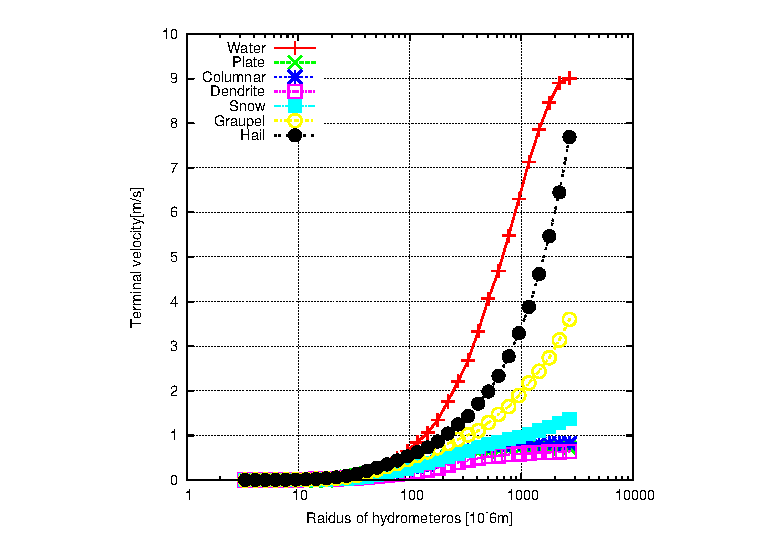
\includegraphics[scale=0.9]{./figure/terminal-velocity.eps}
\end{center}
\caption{Terminal velocity of Water (Plus), Plate-type ice (Cross), Columnar-type ice (Asterisk), Dendrite-type ice(Open square), Snow(Closed square), Graupel(Open circle), and Hail(Closed circle)}
\end{figure}


Although the stochastic collision equation can be apply for collision/coagulation of one type of hydrometeros (i.e. liquid water), the SCALE-LES3 predicts 7 types of hydrometeors, and interactions of these types hydrometeors (i.e. riming/aggregation) must be calculated. To calculate the interaction of all 7 types of hydrometeors, the extented stochastic collision equation:

\begin{eqnarray}
\Bigr[\frac{\partial f^{(\mu)}(m)}{\partial t}\Bigr]_{coll/coag/rim/agg}&=&\nonumber\\
\sum_{\lambda}\sum_{\nu}\int_{0}^{m/2}f^{(\lambda)}&(&m')f^{(\nu)}(m-m')K_{\lambda\nu}(m',m-m')dm' \nonumber\\
-f^{(\mu)}(m)\sum_{\kappa}\int_0^{\infty}f^{(\kappa)}&(&m'')K_{\kappa\mu}(m,m'')dm''
\end{eqnarray}

is applied (where $\mu$, $\nu$, $\lambda$, $\kappa$ represent species of hydrometeor). The convinations of $\mu$, $\nu$, $\lambda$ are shown in table 4.1.

\begin{table}[h]
\begin{center}
\caption{Catalog of interaction between 7 species. W, I, S, G, H shows water, ice, snow, graupel, and hail, respectively. G/H shows graupel(hail) generates when T is lower(higher) than 270.15}
\begin{tabular}{cccccc}
\hline
     & W   & I   & S   & G   & H   \\ \hline\hline
W    & W   & G/H & G/H & G/H & G/H \\ \hline
I    & I   & S   & S   & I   & I   \\ \hline
S    & S   & S   & S   & S   & S   \\ \hline
G    & G/H & G/H & G   & G   & G/H \\ \hline
H    & G/H & G/H & G/H & G/H & H   \\ \hline
\end{tabular}
\end{center}
\end{table}


To solve the stochastic collision equation, a scheme developed by Bott (1998) was implemented into SCLAE-LES3.\\
The Bott (1998) scheme calculate evolution of mass density distribution ($g(\eta)=mf(\eta)$, $\eta=\log(m)$). The stochastic collision equation can be transferred to

\begin{eqnarray}
\frac{\partial g(\eta)}{\partial t}&=&\int_{\eta_{0}}^{\eta_{1}}\frac{m^{2}}{(m-m')^{2} m'}g(\eta-\eta') K(\eta-\eta',\eta')g(\eta')d\eta' \nonumber\\
&-&\int_{\eta_{0}}^{\infty} g(\eta)\frac{K(\eta,\eta')}{m'}g(\eta')d\eta'.
\end{eqnarray}

 where $\eta_{1}=\log(m/2)$. Decreases of mass of i-th bin and j-th bin are given by

\begin{eqnarray}
\frac{\partial g_{i}^{(\mu)}}{\partial t}=-\Delta g^{(\mu)}_{i} K_{\mu\nu}(i,j)\frac{g_{j}^{(\nu)}}{m_{j}}\Delta \eta
\end{eqnarray}

and


\begin{eqnarray}
\frac{\partial g_{j}^{(\mu)}}{\partial t}=-\Delta g^{(\nu)}_{j}K_{\mu\nu}(i,j)\frac{g_{i}^{(\mu)}}{m_{i}}\Delta \eta
\end{eqnarray}

respectively. The terms corresponds to the second term of right-hand side of eq.(???). The equation (???) and (???) can transfer to

\begin{eqnarray}
\Delta g_{i}^{(\mu)}=g_{i}^{(\mu)}\Bigl [1-\exp\bigl(-K_{\mu\nu}(i,j)\frac{g^{(\nu)}_{j}}{m_{j}}\Delta \eta\Delta t\bigr) \Bigl]\\
\Delta g_{j}^{(\nu)}=g_{j}^{(\nu)}\Bigl [1-\exp\bigl(-K_{\mu\nu}(i,j)\frac{g^{(\mu)}_{i}}{m_{i}}\Delta \eta\Delta t\bigr) \Bigl].
\end{eqnarray}

The sum of $\Delta g_{i}^{(\mu)}$ and $\Delta g_{j}^{(\nu)}$ corresponds to newley generated mass by collision of hydrometeor whose mass is $m_{i}$ and $m_{j}$. The newly generated mass ($g'=\Delta g_{i}^{(\mu)}+\Delta g_{j}^{(\nu)}$, which is coresponding to first term of right-hand side of eq.(???)) added k-th bin ($m_{k}=m_{i}+m_{j}$). Since $m_{k}$ is not always bin center, newly generated mass is devided to k-th and k+1-th bin as follow.\\
The production of k-th and k+1-th bin is represened:

\begin{eqnarray}
\Delta g_{k}^{(\lambda)}&=&g_{k}^{\lambda}+g'-\zeta\\
\Delta g_{k+1}^{(\lambda)}&=&g_{k+1}^{\lambda}+\zeta\\
\zeta&=&\frac{g'}{g_{k}^{(\lambda)}+g'}\sum_{s=0}^{2}\frac{a_{k,s}}{(s+1)2^{k+1}}[1-(1-2c_{k})^{k+1}]\nonumber\\
c_{k}&=&\frac{m'-m_{k}}{m_{k+1}-m_{k}}\nonumber\\
a_{k,0}&=&-\frac{1}{24}(g_{k+1}^{(\lambda)}-26g_{k}^{(\lambda)}+g_{k-1}^{(\lambda)})\nonumber\\
a_{k,1}&=&-\frac{1}{2}(g_{k+1}^{(\lambda)}-g_{k-1}^{(\lambda)})\nonumber\\
a_{k,2}&=&-\frac{1}{2}(g_{k+1}^{(\lambda)}-2g_{k}^{(\lambda)}+g_{k-1}^{(\lambda)})\nonumber
\end{eqnarray}

These procedure is applied for all bin of all types of hydrometeors.\\
In addition, to calculate this process fastly, a scheme of Sato et al. (2009) are also implemented into SCALE-LES3.

\subsubsection{Freezing}
The calculation of freezing process is based on a parameterization of Bigg (1953). The parameterization is calculated number density of water ($f_{c}^{(w)}$), wchich can be freezed:

\begin{eqnarray}
\frac{\partial}{\partial t}f^{(w)}(m)&=&-\frac{f^{(w)}(m)}{\tau_{fr}}\\
\tau_{fr}&=&\frac{\exp \bigl[b_{fr}(T_{0}-T)\bigr]}{a_{fr} m}\nonumber
\end{eqnarray}

where $a_{fr}=10^{-4}s^{-1}$, and $b_{fr}=0.66^{o}C^{-1}$ are emperical parameters, and $T_{0}$ is 273.15 $K$.\\
The equation (???) can transfer to

\begin{eqnarray}
\frac{\partial g^{(w)(m)}}{\partial t}&=&-\frac{g^{(w)}(m)}{\tau_{fr}(m)}\\
\tau_{fr,i}&=&\frac{\exp\bigl (b_{fr}(T_{0}-T)\bigr )}{a_{fr}m}\nonumber
\end{eqnarray}

From this equation, The mass change of i-th bin during $\Delta t$ is given as

\begin{eqnarray}
g_{i}^{(w)}(t+\Delta t)=g_{i}^{(w)}-Frz_{i}\\
\left \{
\begin{array}{r}
g_{i}^{(plate)}(t+\Delta t)=g_{i}^{(plate)}+Frz_{i}\:\:\: (r_{w}<200\mu m)\\
g_{i}^{(hail)}(t+\Delta t)=g_{i}^{(hail)}+Frz_{i}\:\:\: (r_{w}>200\mu m)
\end{array} \right.\\
Frz_{i}=g_{i}^{(w)}(t)\Bigl [1-\exp\bigl (-\frac{\Delta t}{\tau_{fr,i}}\bigr )\bigr]\nonumber
\end{eqnarray}


 As shown in equation (???), the mass of liuid is transfer from to plate type ice ($r_{w}<200\mu m$) or hail ($r_{w}>200\mu m$).

\subsubsection{Melting}
The calculation of melting process is too simple way, that is, all ice particles (i.e. plate, columner, dendrite, snow, graupel and hail) melt immediately when the temperature is larger than $T_{0}=273.15$ $K$. This is too simply to represent ice phase process, and we will modify this method near future.


\subsection{Kessler Parameterization}
SCALE implements a one-moment bulk microphysical scheme, which treats only warm clouds (cloud and rain). This scheme predicts the mixing ratio of cloud ($Q_{cloud}$) and rain ($Q_{rain}$). Cloud microphysical processes treated in this scheme are saturation adjustment (corresponding to nucleation, evaporation, and cloud condensation), evaporation, auto-conversion, accretion, and sedimentation. The tendency of $Q_{cloud}$, $Q_{rain}$, and $Q_{v}$ (vapor mixing ratio) is as follows:

\begin{eqnarray}
\frac{\partial Q_{cloud}}{\partial t}&=&dQ|_{sat}-dQ|_{auto}-dQ|_{acc}\\
\frac{\partial Q_{rain}}{\partial t}&=&dQ|_{auto}+dQ|_{acc}-dQ|_{evap}-F_{Q_{r}}|_{sed}\\
\frac{\partial Q_{v}}{\partial t}&=&dQ|_{evap}-dQ|_{sat}
\end{eqnarray}

where $dQ|_{sat}$, $dQ|_{auto}$, $dQ|_{acc}$, and $dQ|_{evap}$ represent the mixing ratio tendency by saturation adjustment, auto-conversion, accretion, and evaporation, respectively. $F_{Q_{r}}|_{sed}$ represents flux of $Q_{r}$ by sedimentation.\\ $dQ|_{auto}$, $dQ|_{acc}$, and $dQ|_{evap}$ are given as:

\begin{eqnarray}
dQ_{auto}&=&\left\{
\begin{array}{ll}
Q_{cloud}*10^{-3} & (Q_{cloud}>10^{-3})\\
0 & (else)\\
\end{array}\right.\\
dQ_{acc}&=&2.2\times Q_{cloud}\times Q_{rain}^{0.875}\\
dQ_{evap}&=&\left\{
\begin{array}{ll}
f_{vent} \frac{q_{s}-Q_{cloud}}{q_{s}\rho}\frac{(\rho*Q_{rain})^{0.525}}{5.4\times 10^{5}+\frac{2.55\times 10^{8}}{pq_{s}}} & ( q_{s} > Q_{cloud})\\
0 & (else)\\
\end{array} \right.
\end{eqnarray}

where $f_{vent}$ is the ventilation factor ($f_{vent}=1.6+124.9(\rho Q_{rain})^{0.2046}$), and the unit of $dQ_{***}$ is [kg/kg/s]. $p$, $q_{s}$, and $\rho$ are pressure, saturation vapor mixing ratio, and total density, respectively.\\
$dQ|_{sat}$ is given as:

\begin{eqnarray}
dQ|_{sat}=Q_{v}-q_{s}.
\end{eqnarray}

Terminal velocities of cloud ($V_{t,c}$) and rain ($V_{t,r}$) are given as:

\begin{eqnarray}
V_{t,c}&=&0\\
V_{t,r}&=&36.34(\rho Q_{rain})^{0.1364} [m/s]
\end{eqnarray}



\subsection{Six-class Single-moment Bulk Scheme (Tomita 2008)}
ix-class single-moment bulk scheme in the SCALE was developed by \citet{tomita_2008}. This scheme predicts mass exchange among six categories of water substances (water vapor, cloud water, rain, cloud ice, snow, and graupel), which is largely based on the method of \citet{Lin_etal}. However, there are some modifications from the original method of \citet{Lin_etal}: Both cloud water and cloud ice are generated only by a saturation adjustment process, and wet growth process of graupel is omitted. According to \citet{tomita_2008}, these modifications result in 20\% reduction in computational cost compared to \citet{Lin_etal} without significant changes on physical performance.

\subsection{Double-Moment Bulk scheme}

SCALE implements a double-moment bulk microphysical scheme with six categories (cloud water, rain, cloud ice, snow, and graupel) 
based on \cite{sn_2014} (hereafter SN14).
SN14 is designed to maintain the self consistency of the assumptions regarding particle mass distribution and
the shapes of ice particles throughout cloud microphysical process.
In this scheme, particle mass distributions of each category are expressed as a generalized gamma function and 0-th moments ( number density ) and
1-th moments ( mass concentration ) of the distributions are predicted. 
SN14 calculates microphysical process for nucleation of cloud droplets and cloud ice,
phase change (condensation/evaporation, deposition/sublimation, freezing, melting), and
collection (self-collection, auto-conversion, accretion and breakup).
Precipitation process for SN14 is separated from other microphysical process and calculated using terminal velocity in SCALE.
More details are described in Appendix \ref{app:sn14}.

\subsection{Spectral Bin Model(SBM)}
The Spectral Bin Model (SBM) was developed by \cite{suzuki_2006} and \cite{suzuki_etal_2010}. The model forecasts the Size Distribution Function (SDF) of seven types of hydrometeors (liquid, plate-ice, columnar-ice, dendritic-ice, snow, graupel, and hail). \\
The SBM calculates mass density of the seven types of hydrometeor and one type of aerosol as their SDFs. The SDF of aerosol can be changed by advection and activation (i.e., nucleation from aerosol to cloud) processes. The SDF of hydrometeors can be changed by several growth processes (i.e., activation from aerosol to cloud, condensation/evaporation, collision/coagulation, freezing/melting, ice nucleation, riming, aggregation, advection, and gravitational falling). \\
The time evolution of SDF (number density) of aerosol ($f_{a}(m,t)$) and SDF (number density) of hydrometeor ($f_{c}(m,t)$) are shown as:

\begin{eqnarray}
\frac{\partial f^{(\mu)}_{c}(m,t)}{\partial t}&=&Adv\bigl[f^{(\mu)}_{c}(m,t)\bigr]+Grav\bigl[f^{(\mu)}_{c}(m,t)\bigr]+\Bigl[ \frac{\partial f^{(\mu)}_{c}(m,t)}{\partial t}\Bigr ]_{cloud\;microphysics}\label{s10-1}\\
\frac{\partial f_{a}(m_{a},t)}{\partial t}&=&Adv\bigl[f_{a}(m_{a},t)\bigr]+Grav\bigl[f_{a}(m_{a},t)\bigr]+\Bigl[ \frac{\partial f_{a}(m_{a},t)}{\partial t} \Bigr ]_{cloud\;microphysics}.\label{s10-2}
\end{eqnarray}

where $\mu$ shows type of hydrometeor (the seven types), and $Adv[]$, $Grav[])$ show change of SDF by  advection and gravitational falling. $\Bigl[ \Bigr]_{cloud\;microphysics}$ shows SDF changes by cloud microphysical processes.\\
The time evolution of $f_{c}^{(\mu)}(m,t)$, and $f_{a}(m,t)$ are shown as:

\begin{eqnarray}
\Bigl[ \frac{\partial f_{c}^{(\mu)}(m,t)}{\partial t}\Bigl]_{cloud\;microphysics}&=&\Bigl[\frac{\partial f_{c}^{(\mu)}(m,t)}{\partial t}\Bigr]_{activation}+\Bigl[\frac{\partial f_{c}^{(\mu)}(m,t)}{\partial t}\Bigr]_{cond/evap}\nonumber\\
&+&\Bigl[\frac{\partial f_{c}^{(\mu)}(m,t)}{\partial t}\Bigr]_{coll/coag/rim/agg}\nonumber\\
&+&\Bigl[\frac{\partial f_{c}^{(\mu)}(m,t)}{\partial t}\Bigr]_{frz}+\Bigl[\frac{\partial f_{c}^{(\mu)}(m,t)}{\partial t}\Bigr]_{melt}\nonumber\\
\Bigl[ \frac{\partial f_{a}(m_{a},t)}{\partial t}\Bigl]_{cloud\;microphysics}&=&\Bigl[\frac{\partial f_{a}(m_{a},t)}{\partial t}\Bigr]_{activation}\nonumber
\end{eqnarray}

where $\Bigl[\;\Bigr]_{***}$ show change of SDF by each cloud growth process. The detail of these processes will be provided later.\\
 The change of SDFs by advection and gravitational falling (i.e., first and second terms of eq.(\ref{s10-1}), and (\ref{s10-2}) ) are calculated by dynamical core of SCALE-RM shown in section 3.


\subsubsection{Discretization of Size Distribution Function(SDF)}
The SDF of aerosol and cloud is predicted as mass density of each particle size ($g_{a}(m_{a})$, $g_{c}^{(\mu)}(m)$). However most equations are given as equations of number density of cloud/aerosol ($f_{c}^{(\mu)}(m,t)$, $f_{a}(m_{a},t)$); the mass density of cloud/aerosol is transferred to the number density of cloud/aerosol ($g_{a}(m_{a},t)=m_{a}g_{a}(m_{a},t)$, $g_{c}^{(\mu)}(m,t)=m^{(\mu)}f_{c}^{(\mu)}(m,t)$).\\
To cover a wide size range (i.e., $2\;\mu m$ $\sim$ $3\;mm$), a logarithmically uniform grid system ($log(m)\equiv \eta$, $log(m_{a})\equiv \eta_{a}$) is used. In this system, the relationship, $\frac{m_{i+1}}{m_{i}}=const.$ is satisfied.

\subsubsection{Activation from aerosol to cloud particles (nucleation process)}
The change of SDFs by activation from aerosol to cloud particles is calculated based on Kohler theory \cite{kohler_1936}. Through this process, aerosols with radii larger than the aerosol critical radius ($r_{a,crit}$) are activated to clouds. The critical radius is given as:

\begin{eqnarray}
r_{a,crit}=\bigl( \frac{4}{27}\frac{A^{3}}{B}\frac{1}{S_{w}}\Bigr )^{1/3}, \:\:\:A=\frac{2\sigma}{R_{v}\rho_{L}T},\:\:\: B=i_{v}\frac{M_{v}}{M_{s}}\frac{\rho_{s}}{\rho_{L}}.\label{s10-3}
\end{eqnarray}

where $S_{w}$, $\sigma$, $R_{v}$, $\rho_{L}$, $T$, $i_{v}$, $M_{v}$, $M_{s}$, and $\rho_{s}$ show supersaturation of water, surface tension of water, vapor gas constant, temperature, van't Hoff factor ($=2$), molecular weight of water, molecular weight of aerosol, and density of aerosol, respectively.\\
At each time step, $r_{a,crit}$ is calculated using temperature, and masses of aerosols with radii > $r_{a,crit}$ are removed from SDF of aerosol and 
transferred to SDF of cloud as newly generated cloud particles.\\
The radii of newly generated clouds correspond to those of aerosols, but if the radii of aerosols are smaller than the lower limit of cloud SDF, the radii of newly generated clouds are set to the smallest size of cloud SDF ($\sim 2 \mu m$).\\
The changes in aerosol and hydrometeor SDF are shown as:

\begin{eqnarray}
\Bigl[\frac{\partial f_{a}}{\partial t}\Bigr]_{activation}&=&-\int_{m_{a,crit}}^{\infty}f_{a}(m_{a},t)dm_{a}\label{s10-4}\\
\Bigl[\frac{\partial f_{c}^{(\mu)}}{\partial t}\Bigr]_{activation}&=&-\Bigl[\frac{\partial f_{a}}{\partial t}\Bigr]_{activation}\label{s10-5}
\end{eqnarray}

where $m_{a,crit}=\bigl(=\frac{4\pi}{3}r_{a}^{3}\rho_{a}$ is mass of aerosol particles with radii the same as critical radii, $r_{a,crit}$. When there is not enough vapor to activate all aerosol particles with radii larger than the critical radius, i.e.,

\begin{eqnarray}
\int_{m_{a,crit}}^{\infty}m_{a}f_{a}(m_{a},t)dm_{a} > q_{v}\rho,\label{s10-6}
\end{eqnarray}

only the aerosol particles with radii > than $r_{a0,crit}$, given as:

\begin{eqnarray}
\int_{m_{a0,crit}}^{\infty}m_{a}f_{a}(m_{a},t)dm_{a} = q_{v}\rho,\label{s10-7}
\end{eqnarray}


are transferred to cloud particles as:

\begin{eqnarray}
\Bigl[\frac{\partial f_{a}}{\partial t}\Bigr]_{activation}&=&-\int_{m_{a0,crit}}^{\infty}f_{a}(m_{a},t)dm_{a},\label{s10-8}\\
\Bigl[\frac{\partial f_{c}^{(\mu)}}{\partial t}\Bigr]_{activation}&=&-\Bigl[\frac{\partial f_{a}}{\partial t}\Bigr]_{activation}.\label{s10-9}
\end{eqnarray}

where $q_{v}$ and $\rho$ is the mixing ratio of water vapor and density.

\subsubsection{Condensation/evaporation}
Calculation of condensation and evaporation processes is based on an equation. The mass change by these two process is given by an equation (e.g., \cite{ry_1989}):

\begin{eqnarray}
\frac{dm}{dt}&=&C^{(\mu)}(m)G^{(\mu)}(T)S^{(\mu)}\\
G^{(\mu)}(T)&=&
\left\{
\begin{array}{l}
G_{w}(T)\;\;\;(\mu : \:liquid)\\
G_{i}(T)\;\;\;(\mu : \:ice)
\end{array}\right. \nonumber\\
G_{w}(T)&=&\frac{4\pi}{\frac{R_{v}T}{e_{w}(T)D_{v}}+\frac{L_{w}}{KT}\bigl( \frac{L_{w}}{R_{v}T}-1\Bigr )}\nonumber\\
G_{i}(T)&=&\frac{4\pi}{\frac{R_{v}T}{e_{i}(T)D_{v}}+\frac{L_{i}}{KT}\bigl( \frac{L_{i}}{R_{v}T}-1\Bigr )}\nonumber\\
S^{(\mu)}&=&
\left\{
\begin{array}{l}
S_{w}\;\;\;(\mu : liquid)\\
S_{i}\;\;\;(\mu : ice)
\end{array}\right.\nonumber
\end{eqnarray}

where $C^{(\mu)}(m)$ is capacitance, which depends on the shape of each type of hydrometeor, $S_{w}$, $S_{i}$ are super saturation of water and ice, $L_{w}$, $L_{i}$ are sensible heat of evaporation, sublimation, $D_{v}$ is diffusion constant of vapor, $K$ is conductivity of air, and $e_{w}$, $e_{i}$ are saturation vapor pressure and saturation ice pressure, respectively. Condensation (evaporation) occur when $S^{(\mu)}$ is positive (negative).\\
To calculate change of SDF by condensation/evaporation, mass flux ($F^{(\mu)}_{cond/evap}$) on each bin is given by using number density ($f_{c}^{(\mu)}$) and $\frac{dm}{dt}$ as:

\begin{eqnarray}
F^{(\mu)}_{cond/evap}=f^{(\mu)}(m)\frac{dm}{dt}=f^{(\mu)}(m)C^{(\mu)}G^{(\mu)}(T)S^{(\mu)}.\label{s10-10}
\end{eqnarray}

Using this equation, time evolution of SDF ($f^{(\mu)}$) is given as

\begin{eqnarray}
\Bigl[\frac{\partial f^{(\mu)}(m,t)}{\partial t}\Bigr]_{cond/evap}&=&-\frac{\partial}{\partial m}F^{(\mu)}_{cond/evap}(m)\nonumber\\
&=&-\frac{\partial}{\partial m}\bigl (f^{(\mu)}(m)C^{(\mu)}\bigr ) G^{(\mu)}(T)S^{(\mu)}.\label{s10-11}
\end{eqnarray}


By using the $\eta(=\log(m))$, eq.(\ref{s10-11}) is transferred to the advection equation:

\begin{eqnarray}
\frac{\partial f^{(\mu)}(\eta)}{\partial t}&=&-\frac{\partial}{\partial \eta}\bigl ( f^{(\mu)}(\eta)U^{(\mu)}(\eta)\bigr)\label{s10-12}\\
U^{(\mu)}(\eta)&=&\frac{C^{(\mu)}(\eta)}{\exp (\eta)}G^{(\eta)}(T)S^{(\eta)}.\nonumber
\end{eqnarray}

To solve eq.(\ref{s10-12}), a scheme developed by \cite{bott_1989} is used. The number density of the i-th bin after $\Delta t$ ($f_{i}(t+\Delta t)$) is given as follows:

\begin{eqnarray}
f_{i}(t+\Delta t)&=&f_{i}(t)-\frac{\Delta t}{\Delta \eta}\bigl [F_{cond/evap,i+1/2}-F_{cond/evap,i-1/2}\Bigr ].\nonumber\\
F_{cond/evap,i+1/2}&=&\frac{\Delta \eta}{\Delta t}\Bigl[ \frac{i^{+}_{l,i+1/2}}{i_{l,j}}f_{i}(t)-\frac{i^{-}_{l,i+1/2}}{i_{l,i+1}}f_{i+1}(t)\Bigr ]\nonumber\\
i^{+}_{l,i+1/2}&=&max\bigl(0,I^{+}_{l}(c_{i+1/2})\bigr)\nonumber\\
i^{-}_{l,i+1/2}&=&max\bigl(0,I^{-}_{l}(c_{i+1/2})\bigr)\nonumber\\
i^{+}_{l,i}&=&max\bigl(I_{l,i},i^{+}_{l,i+1/2}+i^{-}_{l,i+1/2})\bigr)\nonumber\\
I^{+}_{l}(c_{i+1/2})&=&\sum_{k=0}^{2}\frac{a_{i,k}}{(k+1)2^{k+1}}\bigl[1-(1-2c^{+}_{j})^{k+1}\bigr]\nonumber\\
I^{-}_{l}(c_{i+1/2})&=&\sum_{k=0}^{2}\frac{a_{i+1,k}}{(k+1)2^{k+1}}(-1)^{k}\bigl[1-(1-2c^{-}_{j})^{k+1}\bigr]\nonumber\\
a_{i,0}&=&-\frac{1}{24}\bigl( f_{i+1}(t)-26f_{i}(t)+f_{i-1}(t) \bigr)\nonumber\\
a_{i,1}&=&\frac{1}{2}\bigl( f_{i+1}(t)-f_{i-1}(t) \bigr)\nonumber\\
a_{i,2}&=&\frac{1}{2}\bigl( f_{i+1}(t)-2f_{i}(t)+f_{i-1}(t) \bigr)\nonumber\\
c_{i}^{\pm}&=&\pm\bigl( c^{n}_{i+1/2}\pm | c^{n}_{i+1/2}|\bigr )/2\nonumber\\
c^{n}_{i+1/2}&=&U^{n}_{i+1/2}\frac{\Delta t}{\Delta \eta}
\end{eqnarray}

Since super saturation ($S^{(\mu)}$) can change during time step ($\Delta t$), we apply a method shown below to reflect the change of supersaturation during $\Delta t$.\\
Time evolution of supersaturation can be given by equations:

\begin{eqnarray}
\frac{d}{dt}\left(
\begin{array}{l}
S_{w}\\
S_{i}\\
\end{array}\right )
&=&
\left(
\begin{array}{cc}
a_{c/e}& b_{c/e}\\
c_{c/e}& d_{c/e}
\end{array}\right)
\left(
\begin{array}{l}
S_{w}\\
S_{i}
\end{array}\right)
=
A
\left(
\begin{array}{l}
S_{w}\\
S_{i}
\end{array}\right)\label{s10-13}\\
a_{c/e}&=&-(S_{w}+1)\Bigl(\frac{1}{q_{v}}+\frac{L_{w}}{R_{v}T^{2}}\frac{L_{w}}{C_{p}}\Bigr )\int f^{(w)}(m)C^{(w)}(m)dm G_{w}(t)\nonumber\\
b_{c/e}&=&-(S_{w}+1)\Bigl(\frac{1}{q_{v}}+\frac{L_{w}}{R_{v}T^{2}}\frac{L_{i}}{C_{p}}\Bigr ) \sum_{\mu \in ice}\int f^{(\mu)}(m)C^{(\mu)}(m)dm G_{i}(t)\nonumber\\
c_{c/e}&=&-(S_{i}+1)\Bigl(\frac{1}{q_{v}}+\frac{L_{i}}{R_{v}T^{2}}\frac{L_{w}}{C_{p}}\Bigr ) \int f^{(w)}(m)C^{(w)}(m)dm G_{w}(t)\nonumber\\
d_{c/e}&=&-(S_{i}+1)\Bigl(\frac{1}{q_{v}}+\frac{L_{i}}{R_{v}T^{2}}\frac{L_{i}}{C_{p}}\Bigr ) \sum_{\mu \in ice}\int f^{(\mu)}(m)C^{(^mu)}(m)dm G_{i}(t)\nonumber
\end{eqnarray}


where $q_{v}$ is the mixing ratio of vapor. \\
Using eigen value of $A$ ($\Lambda_{+}$, $\Lambda_{-}$ ($\Lambda_{+}>\Lambda_{-})$), and assuming $a_{c/e}$, $b_{c/e}$, $c_{c/e}$, $d_{c/e}$ are constant during $\Delta t$, average value of super saturation ($\bar{S}_{w,i}(t)$) during $\Delta t$ is given as:

\begin{eqnarray}
\bar{S}_{w}(t)=\frac{1}{\Delta t}\int_{t}^{t+\Delta t}S_{w}(\tau)d\tau&=&b\frac{e^{\Lambda_{+}\Delta t}-1}{\Lambda_{+}\Delta t}S_{+}(t)+b\frac{e^{\Lambda_{-}\Delta t}-1}{\Lambda_{-}\Delta t}S_{-}(t)\nonumber\\
\bar{S}_{i}(t)=\frac{1}{\Delta t}\int_{t}^{t+\Delta t}S_{i}(\tau)d\tau&=&(\Lambda_{+}-a)\frac{e^{\Lambda_{+}\Delta t}-1}{\Lambda_{+}\Delta t}S_{+}(t)+(\Lambda_{-}-a)\frac{e^{\Lambda_{-}\Delta t}-1}{\Lambda_{-}\Delta t}S_{-}(t)\nonumber\\
S_{+}(t)&=&\frac{(\Lambda_{-}-a)S_{w}(t)-bS_{i}(t)}{b(\Lambda_{-}-\Lambda_{+})}\nonumber\\
S_{+}(t)&=&\frac{(a-\Lambda_{+})S_{w}(t)+bS_{i}(t)}{b(\Lambda_{-}-\Lambda_{+})}\nonumber
\end{eqnarray}

The averaged super saturation ($\bar{S}_{w,i}(t)$) is used to solve the eq.(\ref{s10-13}).

\subsubsection{Collision/coagulation/riming/aggregation}
Collision/coagulation processes are calculated by solving stochastic collision equations (e.g., \cite{pk_1997}):

\begin{eqnarray}
\frac{\partial f(m)}{\partial t}&=&\int_0^{m/2}f(m')f(m-m')K(m',m-m')dm' \nonumber\\
&-&f(m)\int_0^{\infty}f(m'')K(m,m'')dm''\label{s10-14}
\end{eqnarray}

where $K(m,m')$ is collection kernel function. Three types of kernel function, i.e., Long type kernel (\cite{long_1974}), Golovin type kernel (\cite{Golovin_1963}), and Hydro-dynamic dynamic kernel as shown in eq.(\ref{s10-15}), are implemented into the SCALE-RM.

\begin{eqnarray}
K(m,m')=\pi(r(m)-r(m'))\left| V(m)-V(m')\right |E_{col}(m,m')E_{coag}(m,m')\label{s10-15}
\end{eqnarray}

where $r(m)$ is radius of hydrometeors with mass $m$ and $V(m)$ is terminal velocity of hydrometeors. The terminal velocity of each species of hydrometeor and each size are shown in Figure \ref{figs10-term} $E_{col}$, and $E_{coag}$ are collision efficiency and coagulation efficiency, respectively.\\

\begin{figure}[ht]
\begin{center}
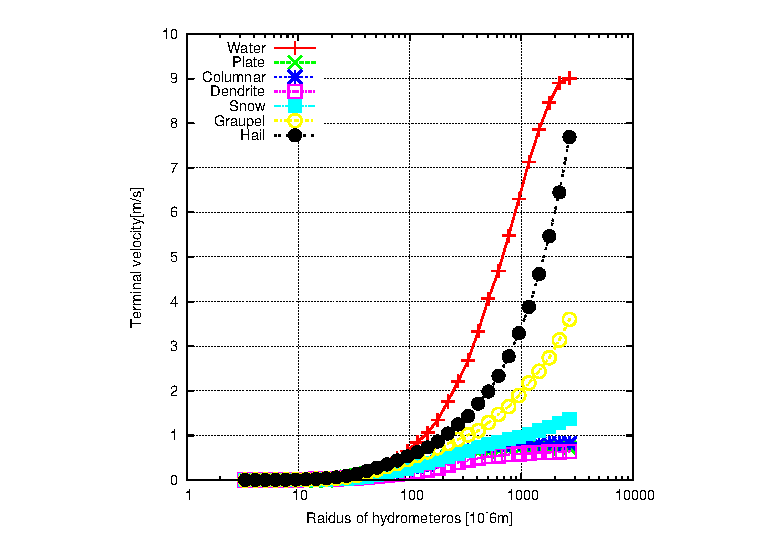
\includegraphics[scale=0.9]{./figure/terminal-velocity.eps}
\end{center}
\caption{Terminal velocity of Water (Plus), plate-type ice (cross), columnar-type ice (asterisk), dendritic-type ice (open square), snow (closed square), graupel (open circle), and hail (closed circle). Cited from Figure A3 of \cite{suzuki_2006} and rearranged.}
\label{figs10-term}
\end{figure}


Although the stochastic collision equation can be applied for collision/coagulation of one type of hydrometeor (i.e., liquid water), SCALE-RM predicts seven types of hydrometeors and interactions of these types (i.e., riming/aggregation) must be calculated. To calculate the interaction of all seven types of hydrometeors, the extended stochastic collision equation:

\begin{eqnarray}
\Bigr[\frac{\partial f^{(\mu)}(m)}{\partial t}\Bigr]_{coll/coag/rim/agg}&=&\nonumber\\
\sum_{\lambda}\sum_{\nu}\int_{0}^{m/2}f^{(\lambda)}&(&m')f^{(\nu)}(m-m')K_{\lambda\nu}(m',m-m')dm' \nonumber\\
-f^{(\mu)}(m)\sum_{\kappa}\int_0^{\infty}f^{(\kappa)}&(&m'')K_{\kappa\mu}(m,m'')dm''\label{s10-16}
\end{eqnarray}

is applied (where $\mu$, $\nu$, $\lambda$, $\kappa$ represent species of hydrometeor). The combinations of $\mu$, $\nu$, $\lambda$ are shown in table \ref{table-s10-1}.

\begin{table}[h]
\begin{center}
\caption{Catalog of interaction between seven species. W, I, S, G, and H show water, ice, snow, graupel, and hail, respectively. G/H shows graupel(hail) generated when T is lower(higher) than 270.15 K}
\label{table-s10-1}
\begin{tabular}{cccccc}
\hline
     & W   & I   & S   & G   & H   \\ \hline\hline
W    & W   & G/H & G/H & G/H & G/H \\ \hline
I    & I   & S   & S   & I   & I   \\ \hline
S    & S   & S   & S   & S   & S   \\ \hline
G    & G/H & G/H & G   & G   & G/H \\ \hline
H    & G/H & G/H & G/H & G/H & H   \\ \hline
\end{tabular}
\end{center}
\end{table}


To solve the stochastic collision equation, a scheme developed by \cite{bott_1998} was implemented into SCALE-RM.\\
The \cite{bott_1998} scheme calculates evolution of mass density distribution ($g(\eta)=mf(\eta)$, $\eta=\log(m)$). The stochastic collision equation can be transferred to:

\begin{eqnarray}
\frac{\partial g(\eta)}{\partial t}&=&\int_{\eta_{0}}^{\eta_{1}}\frac{m^{2}}{(m-m')^{2} m'}g(\eta-\eta') K(\eta-\eta',\eta')g(\eta')d\eta' \nonumber\\
&-&\int_{\eta_{0}}^{\infty} g(\eta)\frac{K(\eta,\eta')}{m'}g(\eta')d\eta'.\label{s10-17}
\end{eqnarray}

 where $\eta_{1}=\log(m/2)$. Decreases of mass of i-th bin and j-th bin are given by:

\begin{eqnarray}
\frac{\partial g_{i}^{(\mu)}}{\partial t}=-\Delta g^{(\mu)}_{i} K_{\mu\nu}(i,j)\frac{g_{j}^{(\nu)}}{m_{j}}\Delta \eta\label{s10-18}
\end{eqnarray}

and


\begin{eqnarray}
\frac{\partial g_{j}^{(\mu)}}{\partial t}=-\Delta g^{(\nu)}_{j}K_{\mu\nu}(i,j)\frac{g_{i}^{(\mu)}}{m_{i}}\Delta \eta\label{s10-19}
\end{eqnarray}

respectively. The terms corresponds to the second term of the right-hand side of eq.(\ref{s10-17}). Eqs.(\ref{s10-18}) and (\ref{s10-19}) can transfer to:

\begin{eqnarray}
\Delta g_{i}^{(\mu)}=g_{i}^{(\mu)}\Bigl [1-\exp\bigl(-K_{\mu\nu}(i,j)\frac{g^{(\nu)}_{j}}{m_{j}}\Delta \eta\Delta t\bigr) \Bigl]\label{s10-20}\\
\Delta g_{j}^{(\nu)}=g_{j}^{(\nu)}\Bigl [1-\exp\bigl(-K_{\mu\nu}(i,j)\frac{g^{(\mu)}_{i}}{m_{i}}\Delta \eta\Delta t\bigr) \Bigl].\label{s10-21}
\end{eqnarray}

The sum of $\Delta g_{i}^{(\mu)}$ and $\Delta g_{j}^{(\nu)}$ corresponds to newly generated mass by collision of hydrometeors with mass of $m_{i}$ and $m_{j}$. The newly generated mass ($g'=\Delta g_{i}^{(\mu)}+\Delta g_{j}^{(\nu)}$,  corresponds to the first term of the right-hand side of eq.(\ref{s10-17})) added k-th bin ($m_{k}=m_{i}+m_{j}$). Since $m_{k}$ is not always bin center, newly generated mass is divided to the k-th and k+1-th bin, as follows.\\
The production of k-th and k+1-th bin is represented as:

\begin{eqnarray}
\Delta g_{k}^{(\lambda)}&=&g_{k}^{\lambda}+g'-\zeta\label{s10-22}\\
\Delta g_{k+1}^{(\lambda)}&=&g_{k+1}^{\lambda}+\zeta\label{s10-23}\\
\zeta&=&\frac{g'}{g_{k}^{(\lambda)}+g'}\sum_{s=0}^{2}\frac{a_{k,s}}{(s+1)2^{k+1}}[1-(1-2c_{k})^{k+1}]\nonumber\\
c_{k}&=&\frac{m'-m_{k}}{m_{k+1}-m_{k}}\nonumber\\
a_{k,0}&=&-\frac{1}{24}(g_{k+1}^{(\lambda)}-26g_{k}^{(\lambda)}+g_{k-1}^{(\lambda)})\nonumber\\
a_{k,1}&=&-\frac{1}{2}(g_{k+1}^{(\lambda)}-g_{k-1}^{(\lambda)})\nonumber\\
a_{k,2}&=&-\frac{1}{2}(g_{k+1}^{(\lambda)}-2g_{k}^{(\lambda)}+g_{k-1}^{(\lambda)})\nonumber
\end{eqnarray}

This procedure is applied for all bins of all types of hydrometeors.\\
In addition, for more rapid calculation, \cite{sato_etal_2009}’s scheme is also implemented into SCALE-RM.

\subsubsection{Freezing}
The calculation of the freezing process is based on a parameterization by \cite{bigg_1953}. The parameterization calculates number density of water ($f_{c}^{(w)}$) that can be frozen:

\begin{eqnarray}
\frac{\partial}{\partial t}f^{(w)}(m)&=&-\frac{f^{(w)}(m)}{\tau_{fr}}\label{s10-24}\\
\tau_{fr}&=&\frac{\exp \bigl[b_{fr}(T_{0}-T)\bigr]}{a_{fr} m}\nonumber
\end{eqnarray}

where $a_{fr}=10^{-4}s^{-1}$, and $b_{fr}=0.66^{o}C^{-1}$ are empirical parameters, and $T_{0}$ is 273.15 $K$.\\
Eq.(\ref{s10-24}) can transfer to:

\begin{eqnarray}
\frac{\partial g^{(w)(m)}}{\partial t}&=&-\frac{g^{(w)}(m)}{\tau_{fr}(m)}\\
\tau_{fr,i}&=&\frac{\exp\bigl (b_{fr}(T_{0}-T)\bigr )}{a_{fr}m}\nonumber
\end{eqnarray}

From this equation, the mass change of i-th bin during $\Delta t$ is given as:

\begin{eqnarray}
g_{i}^{(w)}(t+\Delta t)=g_{i}^{(w)}-Frz_{i}\\
\left \{
\begin{array}{r}
g_{i}^{(plate)}(t+\Delta t)=g_{i}^{(plate)}+Frz_{i}\:\:\: (r_{w}<200\mu m)\\
g_{i}^{(hail)}(t+\Delta t)=g_{i}^{(hail)}+Frz_{i}\:\:\: (r_{w}>200\mu m)
\end{array} \right.\label{s10-26}\\
Frz_{i}=g_{i}^{(w)}(t)\Bigl [1-\exp\bigl (-\frac{\Delta t}{\tau_{fr,i}}\bigr )\bigr]\nonumber
\end{eqnarray}


 As shown in eq.(\ref{s10-26}), the mass of liquid is transferred to plate type ice ($r_{w}<200\mu m$) or hail ($r_{w}>200\mu m$).

\subsubsection{Melting}
The calculation of the melting process is too simple, with all ice particles (i.e., plate, columnar, dendritic, snow, graupel and hail) melting immediately when the temperature is > $T_{0}=273.15$ $K$. This is too simplistic to represent ice phase processes, and we will modify this method in the near future.




\section{Radiation}
%\section{Radiation}
{\bf \Large
\begin{tabular}{ccc}
\hline
  Corresponding author & : & Hisashi Yashiro\\
\hline
\end{tabular}
}
\\

\subsection{mstrnX}
SCALE implements a broadband atmospheric radiative transfer model named ``Model Simulation radiation TRaNsfer code version X (mstrn-X)'' developed by \citet{nakajima_2000} and \citet{sekiguchi_2008}. \verb|mstrn| is based on the discrete ordinate method with a delta two-stream approximation and the correlated k-distribution method. The model calculates long- and short-wave radiation fluxes using the atmospheric states, the three dimensional distribution of clouds/gases/aerosols, and the property of land/ocean surface.
The spectrum between 0.2 and \SI{200}{\micro m} is divided into 29 spectral bands and 111 integration points.

The calculation of solar insolation is based on the parameterization of \citet{berger_1978}. The expected top of atmosphere in the radiation model is 100 km above sea level. However, it is sometimes higher than the top of the domain used in the limited-area simulations.
Thus, SCALE can add the climatological profile to the upper part of the model domain, as needed. The COSPAR International Reference Atmosphere (CIRA-86)  \citep{CSR_2006} is used for the climatological profile of temperature and pressure. The standard profiles of trace gases such as oxygen, carbon dioxide, ozone, water vapor, methane, etc., are referred to the MIPAS reference atmospheres (\citet{Remedios_2007}).


\section{Surface flux}
\section{Surface flux}
{\bf \Large 
\begin{tabular}{ccc}
\hline
  Corresponding author & : & Seiya Nishizawa\\
\hline
\end{tabular}
}


\subsection{Monin-Obukhov similarity}
The first of the all,
we assume that in the boundary layer
1. fluxes are constant,
and 2. variables are horizontally uniform.


Relations between flux and vertical gradient are
\begin{align}
  \frac{kz}{u_*} \frac{\partial u}{\partial z} &= \phi_m\left(\frac{z}{L}\right), \label{eq: flux-gradient u} \\
  \frac{kz}{\theta_*} \frac{\partial \theta}{\partial z} &= \phi_h\left(\frac{z}{L}\right), \label{eq: flux-gradient t} \\
  \frac{kz}{q_*} \frac{\partial q}{\partial z} &= \phi_q\left(\frac{z}{L}\right),
\end{align}
where $k$ is the Von Karman constant.
$L$ is the Monin-Obukhov scale height, which is
\begin{equation}
  L = \frac{\theta u_*^2}{kg\theta_*},
\end{equation}
where $g$ is the gravity.
The scaling velocity, $u_*$, temperature, $\theta_*$,
and water vapor, $q_*$, are defined
from the vertical eddy fluxes of momentum, sensible heat and water vapor:
\begin{align}
  \overline{u'w'} &= -u_*u_*, \\
  \overline{w'\theta'} &= - u_*\theta_*, \\
  \overline{w'q'} &= - u_*q_*.
\end{align}

The integration between the roughness length $z_0$ to the height $z$ of the lowest model level, eqs. (\ref{eq: flux-gradient u}) and (\ref{eq: flux-gradient t}) become
\begin{align}
  u(z) &= \frac{u_*}{k} \left\{\ln(z/z_0)-\Phi_m(z/L)+\Phi_m(z_0/L)\right\}, \\
  \Delta\theta &= R\frac{\theta_*}{k} \left\{\ln(z/z_0)-\Phi_h(z/L)+\Phi_h(z_0/L)\right\},
\end{align}
where $\Delta\theta = \theta-\theta_0$,
and
\begin{align}
  \Phi_m(z) = \int^z \frac{1-\phi_m(z')}{z'} dz', \\
  \Phi_h(z) = \int^z \frac{R-\phi_h(z')}{R z'} dz'.
\end{align}


\subsection{Louis (1979) Model}
Louis (1979) introduced a parametric model of vertical eddy fluxes.

The $L$ becomes
\begin{equation}
  L = \frac{\theta u^2}{g\Delta\theta}
    \frac{\ln(z/z_0)-\Phi_h(z/L)+\Phi_h(z_0/L)}{\left\{\ln(z/z_0)-\Phi_m(z/L)+\Phi_m(z/L)\right\}^2}.
\end{equation}
The bulk Richardson number for the layer $Ri_B$ is
\begin{equation}
  Ri_B = \frac{gz\Delta\theta}{\theta u^2},
\end{equation}
and its form implies relationship with the Monin-Obukhov scale height $L$.
Then the fluxes could be written as
\begin{align}
  u_*^2 &= a^2 u^2 F_m\left(\frac{z}{z_0},Ri_B\right), \label{eq: u_*^2} \\
  u_*\theta_* &= \frac{a^2}{R} u \Delta \theta F_h\left(\frac{z}{z_0},Ri_B\right), \label{eq: u_*t_*}
\end{align}
where
$R$ is ratio of the drag coefficients for momentum and heat in the neutral limit, and
\begin{equation}
  a^2 = \frac{k^2}{\left\{\ln\left(z/z_0\right)\right\}^2}
\end{equation}
is the drag coefficient in neutral conditions.

For the unstable condition ($Ri_B<0$),
$F_i$s ($i=m,h$) could be
\begin{equation}
  F_i = 1 - \frac{b Ri_B}{1 + c_i \sqrt{|Ri_B|}},
\end{equation}
under the consideration that
$F_i$ must behave as $1/u$ (i.e. $\sqrt{|Ri_B|}$) in the free convection limit ($u \to 0$),
and becomes $1$ in neutral conditions ($Ri_B \to 0$).
In the stable conditions ($Ri_b$), on the other hand,
Louis (1979) adopted the following form for $F_i$:
\begin{equation}
  F_i = \frac{1}{(1 + b' Ri_B)^2}.
  \label{eq: F_i stable}
\end{equation}

The constants are estimated as
$R=0.74$ by Businger et al. (1971),
and $b=2b'=9.4$ by Louis (1979).
By the dimensional analysis,
\begin{equation}
  c_i = C^*_i a^2 b \sqrt{\frac{z}{z_0}},
\end{equation}
and $C^*_m = 7.4, C^*_h = 5.3$, which result best fit curves.


\subsection{Uno et al. (1995) Model}
Uno et al. (1995) extended the Louis Model,
which considers difference of the roughness length
between for momentum, $z_0$, and temperature, $z_t$.

The potential temperature difference between $z=z$ and $z=z_t$,
$\Delta\theta_t$, is
\begin{align}
  \Delta\theta_t
  &= R\frac{\theta_*}{k}\left\{\ln(z_0/z_t) - \Phi_h(z_0/L) + \Phi_h(z_t/L)\right\} + \Delta\theta_0, \nonumber \\
  &= R\frac{\theta_*}{k}{\ln(z_0/z_t)} + \Delta\theta_0, \nonumber \\
  &= \Delta\theta_0 \left\{\frac{R\ln(z_0/z_t)}{\Psi_h} + 1\right\},
\end{align}
where $\Delta\theta_0 = \theta_z - \theta_{z_0} (=\Delta\theta)$,
\begin{equation}
  \Psi_h = \int_{z_0}^z\frac{\phi_h}{z'}dz', \label{eq: Psi_h}
\end{equation}
and $\phi_h$ is assumed to be $R$ in the range $z_t < z < z_0$.
Thus
\begin{equation}
  \Delta\theta_0 = \Delta\theta_t \left\{\frac{R\ln(z_0/z_t)}{\Psi_h}+1\right\}^{-1},
  \label{eq: Delta t_0}
\end{equation}
or equivalently,
\begin{equation}
  Ri_{B0} = Ri_{Bt} \left\{\frac{R\ln(z_0/z_t)}{\Psi_h}+1\right\}^{-1}.
  \label{eq: Ri_B0}
\end{equation}

From the eqs. (\ref{eq: u_*^2}) and (\ref{eq: u_*t_*}),
\begin{equation}
  \Delta\theta_0 = \frac{R\theta_*}{k}\ln\left(\frac{z}{z_0}\right)\frac{\sqrt{F_m}}{F_h},
\end{equation}
while
\begin{equation}
  \Delta\theta_0 = \frac{\theta_*}{k}\Psi_h,
\end{equation}
from eqs. (\ref{eq: flux-gradient t}) and (\ref{eq: Psi_h}).
Therefore
\begin{equation}
  \Psi_h = R\ln\left(\frac{z}{z_0}\right)\frac{\sqrt{F_m}}{F_h}.
\end{equation}

Because $\Psi_h$ depends on $Ri_{B0}$,
$Ri_{B0}$ cannot be calculated from $Ri_{Bt}$ with eq. (\ref{eq: Ri_B0})
directly,
so numerical iteration is required to obtain $Ri_{B0}$
\footnote{In the stable case, it can be solved analytically
with eq. (\ref{eq: F_i stable}),
but the solution is too complicated.}.
Starting from $Ri_{Bt}$ as the first estimation of $Ri_{B0}$,
the second estimate by the Newton-Raphson iteration becomes
\begin{equation}
  \hat{Ri}_{B0} = Ri_{Bt} - \frac{Ri_{Bt}R\ln(z_0/z_t)}{\ln(z_0/z_t) + \hat{\Psi_h}},
\end{equation}
where $\hat{\Psi_h}$ is the estimate of $\Psi_h$ using $Ri_{Bt}$ instead of $Ri_{B0}$.
Approximate values for $F_m, F_h$, and $\Psi_h$ are re-calculated
based on the $\hat{Ri}_{B0}$,
and then
$\Delta\theta_0$, and the surface fluxes $u_*^2$ and $u_*\theta_*$
are calculated from eqs. (\ref{eq: Delta t_0}), (\ref{eq: u_*^2}),
and (\ref{eq: u_*t_*}), respectively.


\subsection{Roughness length}
Miller et al. (1992) provides the roughness length over the tropical ocean,
based on the numerical calculations
by combining the smooth surface values with the Charnock relation
for the aerodynamic roughness length
and the constant values for heat and moisture in accordance with Smith (1988,1989) suggestions:
\begin{align}
  z_{0M} &= 0.11u/\nu_* + 0.018u_*^2/g, \\
  z_{0H} &= 0.40u/\nu_* + 1.4 \times 10^{-5}, \\
  z_{0Q} &= 0.62u/\nu_* + 1.3 \times 10^{-4},
\end{align}
where $z_{0M}, z_{0H}$, and $z_{0Q}$ are $z_0$ for the momentum, heat, and vapor,
respectively.


\section{Ocean}
%\section{Land Physics}
{\bf \Large 
\begin{tabular}{ccc}
\hline
  Corresponding author & : & Tsuyoshi Yamaura\\
\hline
\end{tabular}
}


\subsection{Ocean physics: slab model}

The ocean slab model estimates sea temperature tendencies using a single-layered model.
The governing equations of the internal energy $E$ (J/m$^2$) and mass of ocean $M$ (kg/m$^2$) are
\begin{align}
  \frac{\partial E}{\partial t} &= G + e_{prec} - e_{evap} + Q_{ext}, \label{eq:Ocean-Tdt} \\
  \frac{\partial M}{\partial t} &= F_{prec} - F_{evap},
\end{align}
where
$G$ is the downward surface heat flux (J/m$^2$/s);
$e_{prec}$ and $e_{evap}$ are the downward surface internal energy flux (J/m$^2$/s) of the precipitation and evaporation, respectively;
$Q_{ext}$ is external heat source (J/m$^2$/s);
and $F_{prec}$ and $F_{evap}$ are the surface mass flux (kg/m$^2$/s) of the precipitation and evaporation, respectively.

The internal energy E (J/m$^2$) is
\begin{align}
 E = c_l M T,
\end{align}
where $M$ and $T$ are total mass of water (kg/m$^2$) and temperature, and
$c_l$ is the specific heat capacity of water (J/K/kg),


The surface preciptaion flux is
\begin{align}
 F_{prec} &= F_{rain} + F_{snow},
\end{align}
where $F_{rain}$ and $F_{snow}$ are the surface flux of rain and snow, respectively.
The internal energy fluxes are
\begin{align}
 e_{prec} &= c_lT_{rain}F_{rain} + ( c_iT_{snow} - L_f ) F_{snow}, \\
 e_{evap} &= c_lT_{evap}F_{evap},
\end{align}
where $c_i$ is the specific heat capacity of ice (J/K/kg);
$T_{rain}, T_{snow}$ and $T_{evap}$ are the temperature of rain, snow, and evaporated water, respectively;
Note that the fluxes of the rain and snow are positive for the downward direction and that of the evapolation is positive for the upward.
These ground surface fluxes are calculated in the surface scheme.


In the calculation of change of temperature, the mass change is taken into the account.
However, the mass change is ignored after the calculation and then $M = \rho_w D$,
where
$\rho_w$ is the water density (kg/m$^3$),
and $D$ is the water depth of the slab model.

Eq. (\ref{eq:Ocean-Tdt}) is discretized as follows:
\begin{align}
  T^{n+1}
 &= \frac{ C_w T^n + \Delta t ( G + e_{prec} - e_{evap} + Q_{ext} ) }{ C_w + \Delta t c_l ( F_{prec} - F_{evap} ) }, \nonumber\\
 &= T^n + \Delta t \frac{ G + e_{prec} - e_{evap} + Q_{ext} - c_l ( F_{prec} - F_{evap} ) T^n }{ C_w + \Delta t c_l ( F_{prec} - F_{evap} ) },
\end{align}
where
$C_w$ is the heat capacity of the slab layer (J/K/m$^2$) and $C_w = \rho_w c_l D$.

Note that the internal energy is not conserved, since the mass change is ignored.


\subsection{Sea ice}
\subsubsection{Governing equation}
The equations of budget of the mass (kg/m$^2$) and internal energy (J/m$^2$) in the ocean and sea ice are
\begin{align}
 \frac{\partial M_i}{\partial t} &= f_i ( F_{prec}- F_{subl} ) - m_{mlt} + m_{frz}, \\
 \frac{\partial E_i}{\partial t} &= f_i ( G_i - G_{oi} + e_{prec} - e_{subl} ) - c_lT_0m_{mlt} + ( c_iT_0 - L_f ) m_{frz}, \\
 \frac{\partial M}{\partial t} &= (1-f_i) ( F_{prec} - F_{evap} ) + m_{mlt} - m_{frz}, \\
 \frac{\partial E}{\partial t} &= (1-f_i) ( G_o + e_{prec} - e_{evap} ) + f_i G_{oi} + c_lT_0m_{mlt} - ( c_iT_0 - L_f )m_{frz},
\end{align}
where
$f_i$ is the fraction of the sea ice;
$m_{mlt}$ and $m_{frz}$ are the mass change (kg/m$^2$/s) by melting of ice and freezing of sea water;
and $G_i, G_o$ and $G_{oi}$ are the heat flux (J/m$^2$/s) at the ice-atmosphere, ocean-atmosphere, and ice-ocean surfaces, respectively;
$F_{subl}$ is the upward mass flux due to the sublimation of ice (kg/m$^2$/s);
and $e_{subl}$ is the upward internal energy flux at the surface (J/m$^2$/s) of the sublimated ice as
\begin{align}
 e_{subl} &= (c_iT_{subl}-L_f)F_{subl}.
\end{align}

As noted in the previous section, the mass change in the sea water is ignored after the calculation of change in the ocean temperature.

The $G_{oi}$ is estimated by the diffusion equation
\begin{align}
 G_{oi} &= \nu_i \frac{T_i - T}{D_i/2}, \\
 D_i &= \frac{M_i}{\rho_i f_i},
\end{align}
where $T_i$ is the temperature of the sea ice;
$\nu_i$ and $D_i$ are the thermal conductivity of ice (J/K/m$^3$/s) and depth of the sea ice (m).

The fraction is estimated as
\begin{align}
 f_i &= \sqrt{ \frac{M_i}{M_c} },
\end{align}
where $M_c$ is the critical ice mass (kg/m$^2$).

The amount of the melting during a time step is estimated to  satisfy the conservation of mass and internal energy of the sea ice as
\begin{align}
 M_{mlt} &= \int_t^{t+\Delta t} m_{mlt} dt \nonumber\\
 &= \min\left\{ \max\left\{ \frac{ c_i(T_i-T_0) }{ (c_w-c_i) T_0 + L_f } M_i, 0\right\}, M_i\right\}.
\end{align}

The amount of the freezing is estimated to satisfy the conservation of mass and internal energy of the ocean as
\begin{align}
 M_{frz} &= \int_t^{t+\Delta t} m_{frz} dt \nonumber\\
 &= \min\left\{ \max\left\{ \frac{ c_l \rho_w D ( T_0 - T ) }{ (c_l - c_i)T_0 + L_f }, 0\right\}, \rho_w D\right\},
\end{align}
where $T_0$ is the freezing tempearture.


\subsubsection{Time integration}
The governing equation is solved by a spliting method.
In the first step, the mass and internal energy budgets of the ice without the phase change is solved.
In the second step, the melting of sea ice is estimated by the mass and internal energy conservation.
In the next step, then the temperature change of ocean is calculated in the ocean scheme.
In the last step, the freezing ocean water is estimated and the mass and temperature of ice and ocean is updated.

The followings are the summary of the sequence of calculation.
Here, the superscript ``$n$'' indicates the quantites at the time step $n$, and ``$n_1$'', ``$n_2$'', ``$n_3$'', and ``$n+1$'' are those after calculation of the first, seccond, third and the last step, respectively.


\begin{description}

\item[First step]
\begin{align}
 \Delta M_i^{n_1} &= \Delta t f_i^n ( F_{prec} - F_{subl} ), \\
 \Delta E_i^{n_1} &= \Delta t f_i ( G_i - G_{oi} + e_{prec} - e_{subl} ), \\
 M_i^{n_1} &= M_i^n + \Delta M_i^{n_1}, \\
 T_i^{n_1} &= T_i^n + \frac{ \Delta E_i^{n_1} - ( c_iT_i^n - L_f ) \Delta M_i^{n_1} }{c_i M_i^{n_1}}.
\end{align}

\item[Second step]
\begin{align}
 M_{mlt} &= \min\left\{ \max\left\{ \frac{ c_i(T_i^{n_1}-T_0)M_i^{n_1} }{ (c_w-c_i) T_0 + L_f }, 0\right\}, M_i^{n_1}\right\}, \\
 M_i^{n_2} &= M_i^{n_1} - M_{mlt}, \\
 T_i^{n_2} &= T_i^{n_1} + \frac{ - c_l T_0  + ( c_iT_i^{n_1} - L_f )}{c_i M_i^{n_2}}M_{mlt}.
\end{align}

\item[Third step] (Ocean model)
\begin{align}
 \Delta E^{n_3} &= \Delta t \{ (1-f_i)(G_o + e_{prec} - e_{evap}) + f_i G_{oi} \} + c_l T_0 M_{mlt}, \\
 \Delta M^{n_3} &= \Delta t (1-f_i)(F_{prec}-F_{evap}) + M_{mlt}, \\
 T^{n_3} &= T^n + \frac{ \Delta E^{n_3} - c_l T^n \Delta M^{n_3} }{c_l \{\rho_w D + \Delta M^{n_3} \}}.
\end{align}

\item[Forth step]
\begin{align}
 M_{frz} &= \min\left\{ \max\left\{ \frac{ c_l \rho_w D ( T_0 - T^{n_3} ) }{ (c_l - c_i)T_0 + L_f }, 0\right\}, \rho_w D\right\}, \\
 M_i^{n+1} &= M_i^{n_2} + M_{frz}, \\
 T_i^{n+1} &= T_i^{n_3} + ( T_0 - T_i^{n_3} ) \frac{M_{frz}}{M_i^{n+1}}, \\
 T^{n+1} &= T^{n_3} + \frac{ - ( c_i T_0 - L_f ) + c_l T^{n_3} }{c_l (\rho_w D - M_{frz}) } M_{frz}.
\end{align}

\end{description}

\subsection{Sea surface albedo}
\subsubsection{Nakajima et al. (2000) model}
\citet{nakajima_2000} provided the albedo for the short wave on the sea surface $A$:
\begin{align}
  A = \exp \left[ \Sigma_{i=1}^{3} \Sigma_{j=1}^{5} C_{ij} t^{j-1} \mu_0^{i-1} \right],
\end{align}
where
$C_{ij}$ is the empirical optical parameters,
$t$ is the flux transmissivity for short-wave radiation,
and $\mu_0$ is cosine of the solar zenith angle.


\subsection{Roughness length}
\subsubsection{Miller et al. (1992) model}
\citet{miller_1992} provides the roughness length over the tropical ocean,
based on numerical calculations by combining smooth surface values
with the Charnock relation for aerodynamic roughness length
and constant values for heat and moisture in accordance with \citet{Smith_1988,Smith_1989} suggestions:
\begin{align}
  z_0 &= 0.11u/\nu_* + 0.018u_*^2/g, \label{eq: z_0} \\
  z_t &= 0.40u/\nu_* + 1.4 \times 10^{-5}, \label{eq: z_t} \\
  z_q &= 0.62u/\nu_* + 1.3 \times 10^{-4}, \label{eq: z_q}
\end{align}
where $\nu_*$ is the kinematic viscosity of air ($\sim 1.5 \times 10^{-5}$), and $z_0, z_t$,
and $z_q$ are the roughness length for momentum, heat, and vapor, respectively.

\subsubsection{Moon et al. (2007) model}
\citet{moon_2007} provides the air--sea momentum flux at high wind speeds
based on the coupled wave--wind model simulations for hurricanes.
At first, the wind speed $U$ at 10-m height is estimated from the previous roughness length $z_0$, as follows:
\begin{align}
  U =\frac{u_{*}}{\kappa} \ln \frac{10}{z_0},
\end{align}
where
$u_{*}$ is friction velocity (m/s)
and $\kappa$ is von Kalman constant.
And then, new roughness length $z_0$ is iteratively estimated from the wind speed:
\begin{equation}
  z_0   = \left\{
  \begin{array}{lll}
    \frac{0.0185}{g} u_{*}^2 & \mathrm{for} & U < 12.5, \\
    \left[ 0.085 \left( -0.56 u_{*}^2 + 20.255 u_{*} + 2.458 \right) - 0.58 \right] \times 10^{-3} & \mathrm{for} & U \ge 12.5.
   \end{array} \right.
\end{equation}

Furthermore, \citet{Fairall_2003} provides the roughness length for the heat and vapor
using that for momentum, as follows:
\begin{align}
  z_t &= \frac{ 5.5 \times 10^{-5} }{ ( z_0 u_{*} / \nu_{*} )^{0.6} }, \\
  z_q &= z_t.
\end{align}



\section{Land} \label{sec:land}
%\section{Land Physics}
{\bf \Large 
\begin{tabular}{ccc}
\hline
  Corresponding author & : & Tsuyoshi Yamaura\\
\hline
\end{tabular}
}


\subsection{Land physics: slab model}

The land slab model estimates the tendency of soil temperature and soil moisture with multi-layered bucket model.
The tendency equiation of soil temperature is estimated from the 1-D vertical diffusion equation.
That is,
\begin{align}
  \frac{\partial T}{\partial t} = \frac{1}{\rho_{L}C_{L}} \left\{ \frac{\partial}{\partial z} \left( \kappa \frac{\partial T}{\partial z} \right) + Q \right\},
  \label{eq:Tdt}
\end{align}
where $T$ is soil temperature ($K$), $\rho_{L}$ is land density ($kg/m^3$), $C_{L}$ is land heat capacity ($J/K/kg$), $\kappa$ is thermal conductivity ($J/K/m/s$), and $Q$ is heat source from the outside ($J/m^3/s$).
The eq. (\ref{eq:Tdt}) is discretized as follows:
\begin{align}
  \frac{\Delta T_{k}}{\Delta t} &= \frac{\nu_{k}}{\Delta z_{k}} \left( \frac{T_{k+1}-T_{k}}{\Delta z_{k+\frac{1}{2}}} - \frac{T_{k}-T_{k-1}}{\Delta z_{k-\frac{1}{2}}} \right) + \frac{Q_{k}}{(\rho_{L}C_{L})_{k}}, \\
                                &= \frac{ 2\nu_{k} }{ \Delta z_{k} (\Delta z_{k+1}+\Delta z_{k}) }(T_{k+1}-T_{k}) - \frac{ 2\nu_{k} }{ \Delta z_{k} (\Delta z_{k}+\Delta z_{k-1}) }(T_{k}-T_{k-1}) +\frac{Q_{k}}{(\rho_{L}C_{L})_{k}},
\end{align}
where
\begin{align}
  \nu_{k} &= \frac{\kappa}{(\rho_{L}C_{L})_{k}}, \\
  (\rho_{L}C_{L})_{k} &= ( 1 - S_{max} ) C_{S} + S_{k} \rho_{W}C_{W},
\end{align}
and $S$ is moisture content at $k$-layer ($m^3/m^3$), $S_{max}$ is maximum moisture content, $C_{S}$ and $C_{W}$ are heat capaticity of soil and water ($J/K/kg$), and $\rho_{W}$ is water density ($kg/m^3$).
The range of $k$ is 1 to $m$.
In this case, $m$ is the number of the lowermost layer.
The tendency equations of soil temperature are implemented as follows:
\begin{align}
  \frac{\Delta T_{1}}{\Delta t} &= - \frac{G_{0}}{(\rho_{L}C_{L})_{1}\Delta z_{1}} + \frac{2\nu_{1}}{\Delta z_{1}(\Delta z_{2}+\Delta z_{1})} (T_{2}-T_{1}), \\
  \frac{\Delta T_{k}}{\Delta t} &= - \frac{2\nu_{k}}{\Delta z_{k}(\Delta z_{k}+\Delta z_{k-1})} (T_{k}-T_{k-1}) + \frac{2\nu_{k}}{\Delta z_{k}(\Delta z_{k+1}+\Delta z_{k})} (T_{k+1}-T_{k}), \\
  \frac{\Delta T_{m}}{\Delta t} &= - \frac{2\nu_{m}}{\Delta z_{m}(\Delta z_{m}+\Delta z_{m-1})} (T_{m}-T_{m-1}),
\end{align}
where $G_{0}$ is upward groud heat flux from atmospheric surface ($J/m^2/s$).
We assume that the ground heat flux under the lowermost layer is zero.

We use implicit scheme for the time integration of the land slab model.
The cofficients in the tendency equation are summarized as follows:
\begin{align}
  a_{1} &= 0, \\
  a_{k} &= - \frac{2\nu_{k}\Delta t}{\Delta z_{k}(\Delta z_{k}+\Delta z_{k-1})}, \\
  b_{k} &= - \frac{2\nu_{k}\Delta t}{\Delta z_{k}(\Delta z_{k}+\Delta z_{k+1})}, \\
  b_{m} &= 0.
\end{align}
Then, the tendency equations of soil temperature are reqritten as follows:
\begin{align}
  T_{1}^{t} &= T_{1}^{t-1} - \frac{G_{0}\Delta t}{\rho_{L}C_{L}\Delta z_{1}} + b_{1} (T_{1}^{t}-T_{2}^{t}), \\
  T_{k}^{t} &= T_{k}^{t-1} + a_{k} (T_{k}^{t}-T_{k-1}^{t}) + b_{k} (T_{k}^{t}-T_{k+1}^{t}), \\
  T_{m}^{t} &= T_{m}^{t-1} + a_{m} (T_{m}^{t}-T_{m-1}^{t}).
\end{align}
This simultaneous equation can be written by using matrix. That is,
\begin{equation}
\begin{pmatrix}
  c_{1}  & b_{1}  &        &        &         &         &         \\
  a_{2}  & c_{2}  & b_{2}  &        &         &         &         \\
         & \ddots & \ddots & \ddots &         &         &         \\
         &        & a_{k}  & c_{k}  & b_{k}   &         &         \\
         &        &        & \ddots & \ddots  & \ddots  &         \\
         &        &        &        & a_{m-1} & c_{m-1} & b_{m-1} \\
         &        &        &        &         & a_{m}   & c_{m}   \\
\end{pmatrix}
\begin{pmatrix}
  T_{1}^{t}   \\
  T_{2}^{t}   \\
  \vdots      \\
  T_{k}^{t}   \\
  \vdots      \\
  T_{m-1}^{t} \\
  T_{m}^{t}   \\
\end{pmatrix}
=
\begin{pmatrix}
  T_{1}^{t-1} - \frac{G_{0}\Delta t}{\rho_{L}C_{L}\Delta z_{1}} \\
  T_{2}^{t-1}   \\
  \vdots        \\
  T_{k}^{t-1}   \\
  \vdots        \\
  T_{m-1}^{t-1} \\
  T_{m}^{t-1}   \\
\end{pmatrix}
,
\end{equation}
where $c_{k} = 1 - a_{k} - b_{k}$.
This matrix can be solved by the Thomas algorithm (tridiagonal matrix algorithm).

Soil moisture is estimated by the similar method.
The tendency equations of soil moisture is defined as the 1-D vertical diffusion euqation.
That is,
\begin{align}
  \frac{\partial W}{\partial t} = \frac{\partial}{\partial z} \left( \nu \frac{\partial W}{\partial z} \right),
  \label{eq:Wdt}
\end{align}
where $W$ is soil moisture ($m^3/m^3$) and $\nu$ is constant water diffusivity for $k$ ($m^2/s$).
The eq. (\ref{eq:Wdt}) is discretized as follows:
\begin{align}
  \frac{\Delta W_{1}}{\Delta t} &= \frac{P - E}{\rho_{W}\Delta z_{1}} + \frac{2\nu}{\Delta z_{1}(\Delta z_{2}+\Delta z_{1})} (W_{2}-W_{1}), \\
  \frac{\Delta W_{k}}{\Delta t} &= - \frac{2\nu}{\Delta z_{k}(\Delta z_{k}+\Delta z_{k-1})} (W_{k}-W_{k-1}) + \frac{2\nu}{\Delta z_{k}(\Delta z_{k+1}+\Delta z_{k})} (W_{k+1}-W_{k}), \\
  \frac{\Delta W_{m}}{\Delta t} &= - \frac{2\nu}{\Delta z_{m}(\Delta z_{m}+\Delta z_{m-1})} (W_{m}-W_{m-1}),
\end{align}
where $P$ is precipitation rate ($kg/m^2/s$) and $E$ is evaporation rate ($kg/m^2/s$).
Same as soil temperature, the tendency equations can be solved by the Thomas algorithm.


\section{Urban}
{\bf \Large
\begin{tabular}{ccc}
\hline
  Corresponding author & : & Sachiho A. Adachi\\
\hline
\end{tabular}
}
\\


Urban models calculate energy exchanges between the urban surface (urban canopy) and atmosphere.
SCALE-RM has two options for calculation of urban areas: LAND and KUSAKA01.
In LAND option, fluxes over urban subtiles are calculated by the land model you chose for your examination.
Please refer to Section \ref{sec:land}.

\subsection{KUSAKA01: Single layer urban canopy model}

KUSAKA01 is the single layer urban canopy model by \citet{kusaka_2001} and \citet{kusaka_2004} (henceforth, UCM).
The UCM of KUSAKA01 assumes street canyons as the urban geometry.
The model estimates prognostic variables of the surface temperatures and heat fluxes from three surfaces, i.e., roofs, walls, and roads,
and those from urban canopy.
The model assumes that the urban canopy layer is located lower than the 1st layer of atmospheric model.
Therefore, there is a restriction that a sum of displacement height and roughness length must be two meters lower than the face level of 1st layer of atmosphere.
In this version, single urban type can be considered in the urban model.
Several parameters are prepared to specify the urban geometry and anthropogenic heat. 


%\section{Aerosol}
%\chapter{Aerosol}
{\bf \Large
\begin{tabular}{ccc}
\hline
  Corresponding author & : & Mizuo Kajino\\
\hline
\end{tabular}
}


\section{Large scale sinking}
{\bf \Large 
\begin{tabular}{ccc}
\hline
  Corresponding author & : & Seiya Nishizawa\\
\hline
\end{tabular}
}


In the DYCOMS01 experiment, large scale sinking is added to express large scale downward motion corresponding to the Hadley circulation. There is virtual convergence of motion, resulting in mass escape out of the system.

The density loss rate is constant $L$:
\begin{equation}
  L = -\frac{\partial \rho w_L}{\partial z},
\end{equation}
where $w_l$ is vertical velocity corresponding to large scale sinking.
Vertical momentum with sinking is defined as follows:
\begin{equation}
  \rho w_L = -Lz.
\end{equation}

The continuous equation is now:
\begin{equation}
  \frac{\partial \rho}{\partial t}
  + \frac{\partial \rho u}{\partial x}
  + \frac{\partial \rho v}{\partial y}
  + \frac{\partial \rho (w+w_L)}{\partial z}
  = -L.
  \label{eq: lls rho}
\end{equation}

The Lagrangian conservation equation for scalar quantities is:
\begin{equation}
  \rho\frac{\partial \phi}{\partial t}
  + \rho u\frac{\partial \phi}{\partial x}
  + \rho v\frac{\partial \phi}{\partial y}
  + \rho (w+w_L)\frac{\partial \phi}{\partial z}
  = 0,
\end{equation}
When combined with eq. (\ref{eq: lls rho}), this becomes:
\begin{equation}
  \frac{\partial \rho\phi}{\partial t}
  + \frac{\partial \rho u \phi}{\partial x}
  + \frac{\partial \rho v \phi}{\partial y}
  + \frac{\partial \rho (w+w_L) \phi}{\partial z}
  = -L\phi.
\end{equation}

The equation for the mixing ratio is:
\begin{equation}
  \frac{\partial \rho Q}{\partial t}
  + \frac{\partial \rho Q u }{\partial x}
  + \frac{\partial \rho Q v}{\partial y}
  + \frac{\partial \rho Q (w+w_L)}{\partial z}
  = -L Q.
\end{equation}
Note that this is identical to that for scalar quantities.

The $w_L$ at the top boundary is not zero, while $w$ is zero.
The vertical flux $\rho w_L \phi$ at the top layer interface could be determined as that convergence of the flux canceled with $L\phi$.





\bibliographystyle{plainnat}
\bibliography{reference}

\appendix
\chapter{The detail numerics}
\input{cd4}
\input{fct}

\chapter{Details of Seiki and Nakajima (2014)}
\label{app:sn14}
\input{microphysics_seiki_details}

\chapter{Notation}
\chapter{Notation}

\begin{table}[htbp]
  \caption{Notation of symbols}
  \begin{tabular}{lll}\hline
    $\rho$ & total density                       &  $kg/m^3$\\
    $q_d$  & mass concentration of dry air       &  $-$   \\
    $q_v$  & mass concentration of water vapor   &  $-$   \\
    $q_l$  & mass concentration of liquid water &   $-$   \\
    $q_s$  & mass concentration of solid water &    $-$   \\
    $t$    & time                              &   $s$   \\
    ${\bf u}$  & velocity of air flow          &   $m/s$   \\
    $w_l$  & relative velocity of liquid water to the gas    &   $m/s$   \\
    $w_s$  & relative velocity of solid water to the gas    &    $m/s$   \\
    ${\rm DIFF}\left[ x \right]$  & Diffusion term by turbulene  &    $kg/m^3\left[x\right]/s$   \\
    $S_v$    & source term of water vapor                     &    $kg/m^3/s$   \\
    $S_l$    & source term of liquid water                     &   $kg/m^3/s$   \\
    $S_s$    & source term of solid water                     &    $kg/m^3/s$   \\
    $p$      & pressure                                       &   $N/m^2$  \\
    $g$      & gravitational acceraration                     &   9.8 $m/s^2$ \\
    $f_l$      & drag force due to water loading by liquid water  &   $kg /m^2/s^2$ \\
    $f_s$      & drag force due to water loading by solid water   &   $kg /m^2/s^2$ \\
    ${\bf e_z}$ & vertical unit vector ( upward )                 &  $-$ \\
    $R_d$ & gas constant for dry air for uint mass               &  $J/kg$ \\
    $R_v$ & gas constant for water vapor for uint mass               &  $J/kg$ \\
    $T$   & temperature                                          & $K$ \\
    $Q_d$   & diabatic heating due to physical processes for dry air  & $J/m^3/s$ \\
    $Q_v$   & diabatic heating due to physical processes for water vapor  & $J/m^3/s$ \\
    $Q_l$   & diabatic heating due to physical processes for liquid water  & $J/m^3/s$ \\
    $Q_s$   & diabatic heating due to physical processes for solid water  & $J/m^3/s$ \\
    $e_d$   & internal energy for dry air  & $J/kg$ \\
    $e_v$   & internal energy for water vapor  & $J/kg$ \\
    $e_l$   & internal energy for liquid water & $J/kg$ \\
    $e_s$   & internal energy for solid water & $J/kg$ \\
    $e$   & total internal energy & $J/kg$ \\
    $c_{vd}$   & specific heat at constant volume for dry air & $J/kg/K$ \\
    $c_{vv}$   & specific heat at constant volume for water vapor & $J/kg/K$ \\
    $c_{pd}$   & specific heat at constant pressure for dry air & $J/kg/K$ \\
    $c_{pv}$   & specific heat at constant pressure for water vapor & $J/kg/K$ \\
    $c_l$   & specific heat for liquid water & $J/kg/K$ \\
    $c_s$   & specific heat for solid water & $J/kg/K$ \\
    $p_{00}$   & standard pressure & 1000.0 $Pa$ \\
    $\theta_d $   & potential temperature for dry air&  $K$ \\
    $\theta $   & total potential temperature&  $K$ \\
    \hline
  \end{tabular}
\end{table}


\chapter{Variables in the source code}
\chapter{Variables in the source code}


\begin{table}[htbp]
  \caption{Variables in atmos/mod\_atmos\_dyn\_fent\_fct.f90.}
  \begin{tabular}{ll}\hline
    DENS(k,i,j) & $\rho_{i,j,k}$ \\
    MOMZ(k,i,j) & $(\rho w)_{i,j,k+\frac{1}{2}}$ \\
    MOMX(k,i,j) & $(\rho u)_{i+\frac{1}{2},j,k}$ \\
    MOMY(k,i,j) & $(\rho v)_{i,j+\frac{1}{2},k}$ \\
    RHOT(k,i,j) & $(\rho\theta)_{i,j,k}$ \\
    QTRC(k,i,j,iq) & $q_{i,j,k}$ \\
    PRES(k,i,j) & $p_{i,j,k}$ \\
    VELZ(k,i,j) & $\bar{w}_{i,j,k+\frac{1}{2}}$ \\
    VELX(k,i,j) & $\bar{u}_{i+\frac{1}{2},j,k}$ \\
    VELY(k,i,j) & $\bar{v}_{i,j+\frac{1}{2},k}$ \\
    POTT(k,i,j) & $\theta_{i,j,k}$ \\
    QDRY(k,i,j) & $q_d$ \\
    Rtot(k,i,j) & $R^*$ \\
    num\_diff(k,i,j) & $F_{i+\frac{1}{2}}$ \\
    qflx\_hi(k,i,j) & $\bar{q}^{high}$ \\
    qflx\_lo(k,i,j) & $\bar{q}^{low}$ \\
    qjpls(k,i,j) & $Q^+_{i,j,k}$ \\
    qjmns(k,i,j) & $Q^-_{i,j,k}$ \\
    pjpls(k,i,j) & $P^+_{i,j,k}$ \\
    pjmns(k,i,j) & $P^-_{i,j,k}$ \\
    rjpls(k,i,j) & $R^+_{i,j,k}$ \\
    rjmns(k,i,j) & $R^-_{i,j,k}$ \\
  \hline\end{tabular}
\end{table}


\begin{table}[htbp]
  \caption{Variables in atmos/mod\_atmos\_phy\_tb\_smg.f90.}
  \begin{tabular}{ll}\hline
    tke(k,i,j) & $TKE$ \\
    nu(k,i,j), nu\_*(k,i,j) & $\nu_{SGS}$ \\
    Ri(k,i,j) & $Ri$ \\
    Pr(k,i,j) & $Pr$ \\
    S33\_*(k,i,j) & $S_{33}$ \\
    S11\_*(k,i,j) & $S_{11}$ \\
    S22\_*(k,i,j) & $S_{22}$ \\
    S31\_*(k,i,j) & $S_{31}$ \\
    S12\_*(k,i,j) & $S_{12}$ \\
    S23\_*(k,i,j) & $S_{23}$ \\
    qflx\_sgs(k,i,j) & $\bar{\rho}\tau_{ij}$, $\bar{\rho}\tau^*_{ij}$ \\
  \hline\end{tabular}
\end{table}



\end{document}

